\documentclass[oneside]{tongjithesis} % 双面模式请将 oneside 改为 twoside
\usepackage{tongjithesis}
\usepackage{ulem}
\usepackage{makecell}
\usepackage{hyperref}
\begin{document}

\school{电子信息与工程学院}
\major{数据科学与大数据技术}
\student{}{范潇(2254298)}
\thesistitle{在 UNIX V6++中添加新的系统调用}{}
\thesistitleeng{Thesis Template}{with Various Scenes}
% \thesisadvisor{某某某}
\thesisdate{2024}{11}{13}

\MakeCover

\cleardoublepage

% \pagestyle{firststyle}
% \MakeAbstract{
    摘要通常是一篇文章、论文、报告或其他文本的简短概括。它的目的是帮助读者了解文本的主要内容和结论,以便决定是否需要继续阅读原文。摘要通常包含文本的主题、目的、方法、结果和结论等方面的信息,并尽可能简洁明了地呈现。好的摘要应该能够概括文本的重点,同时避免使用不必要的细节和专业术语,以便广大读者能够轻松理解。

    此外,摘要通常也是学术界和研究人员评估一篇文献的重要依据之一。在文献检索和筛选过程中,人们通常会根据摘要来决定是否进一步查看完整的文献。因此,撰写一个清晰、准确、简洁的摘要对于文献的传播和影响力至关重要。在撰写摘要时,作者应该遵循文献的格式要求和撰写规范,同时结合文本的内容和目的,将摘要撰写得准确、简洁、易懂,以提高文献的传播和影响力。

    关键词1,关键词2,关键词3通常是与文章内容相关的几个词语,用于帮助读者更好地了解文章主题和内容。关键词的选择应该与文章的主题和研究领域密切相关,通常应该选择具有代表性、权威性、独特性和可搜索性的词语。
}{关键词1,关键词2,关键词3}

\MakeAbstractEng{
    An abstract is usually a short summary of an article, essay, report, or other text. Its purpose is to help the reader understand the main content and conclusions of the text so that he or she can decide whether he or she needs to continue reading the original text. The abstract usually contains information about the topic, purpose, methods, results, and conclusions of the text and is presented as concisely and clearly as possible. A good abstract should be able to summarize the main points of the text while avoiding unnecessary details and jargon so that it can be easily understood by a wide audience.

    In addition, abstracts are often one of the most important bases on which academics and researchers evaluate a piece of literature. During the literature search and selection process, people often base their decision to look further into the complete literature on the abstract. Therefore, writing a clear, accurate, and concise abstract is crucial to the dissemination and impact of the literature. When writing an abstract, authors should follow the formatting requirements and writing specifications of the literature, as well as combine the content and purpose of the text to write an accurate, concise, and easy-to-understand abstract in order to improve the dissemination and impact of the literature.

    Keyword 1, Keyword 2, and Keyword 3 are usually a few words related to the content of the article and are used to help readers better understand the topic and content of the article. The choice of keywords should be closely related to the topic and research area of the article, and words that are representative, authoritative, unique, and searchable should usually be chosen.
}{Keyword 1, Keyword 2, Keyword 3}


\clearpage
\pagestyle{firststyle}
\tableofcontents   %放置目录
\cleardoublepage

\pagestyle{mainstyle}
\section{项目背景}

随着互联网技术的快速发展和数字化转型的深入推进,大数据分析在各个领域的应用日益广泛。在人力资源和招聘领域,数据驱动的决策支持变得尤为重要。当前的就业市场面临着信息分散、数据孤岛等挑战,不同招聘平台之间的数据壁垒阻碍了就业市场的整体分析和研究。

在当前的就业市场中,存在以下突出问题:

\begin{itemize}
    \item 信息分散:招聘信息分布在多个平台,增加了信息获取成本
    \item 数据割裂:不同平台的数据格式不统一,难以进行综合分析
    \item 可视化不足:传统招聘网站以列表形式展示信息,缺乏直观的数据可视化
    \item 分析深度不够:现有平台主要提供基础的搜索功能,缺乏深度的数据分析
\end{itemize}
\chapter{需求分析}\label{chap:feasibility}
\thispagestyle{empty}
\section{功能需求}
% 本平台的用户可以分为三类:分析团队、调度员和管理者。

对于分析团队,他们对该平台有以下需求:
\begin{enumerate}
    \item 由平台生成查看单车分布图,对应图\ref{GenerateBikeDistributionMap}中的用例\texttt{Generate Bike Distribution Map};
    \item 由平台生成调度日志,对应图\ref{ProduceBikeSchedulingLog}中的用例\texttt{Produce Bike Scheduling Log};
    \item 由平台生成单车使用情况的空间分布,对应图\ref{GenerateBikeUsageMap}中的用例\texttt{Generate Bike Usage Map}。
    \item 由平台生成单车状况统计信息,对应图\ref{ProduceBikeStatusStatistics}中的用例\texttt{Produce Bike Status Statistics}。
\end{enumerate}

对于调度员,他们对于该平台有以下需求:
\begin{enumerate}
    \item 调度员可以在平台中上传调度信息,对应图\ref{UploadSchedulingLog}中的用例\texttt{Upload Scheduling Log};
    \item 调度员可以在平台中更新单车状态信息,对应图\ref{UpdateSingleBikeStatus}中的用例\texttt{Update Single Bike Status}。
\end{enumerate}

对于管理者,在分析团队的需求基础之上,他们对于该平台有还以下需求:
\begin{enumerate}
    \item 管理者可以通过平台添加或删除单车信息,对应图\ref{ModifyBikeList}中的用例\texttt{Modify Bike List};
    \item 管理者可以通过平台添加或删除停车区域信息,对应图\ref{ModifyParkingAreaList}中的用例\texttt{Modify Parking Area List}。
    \item 通过平台全局更新单车状态,对应图\ref{UpdateBikeStatusGlobally}中的用例\texttt{Update Bike Status Globally}。
\end{enumerate}

处于安全性考虑,平台还需要对上述三类用户进行分级。

同时,该平台需要处理由共享单车在开关锁时上传的信息,对应图\ref{UpdateBikeInformation}中的用例\texttt{Update Bike Info}。

整个系统的用例汇总如图\ref{UseCase}所示。

\begin{figure}[!htbp]
    \centering
    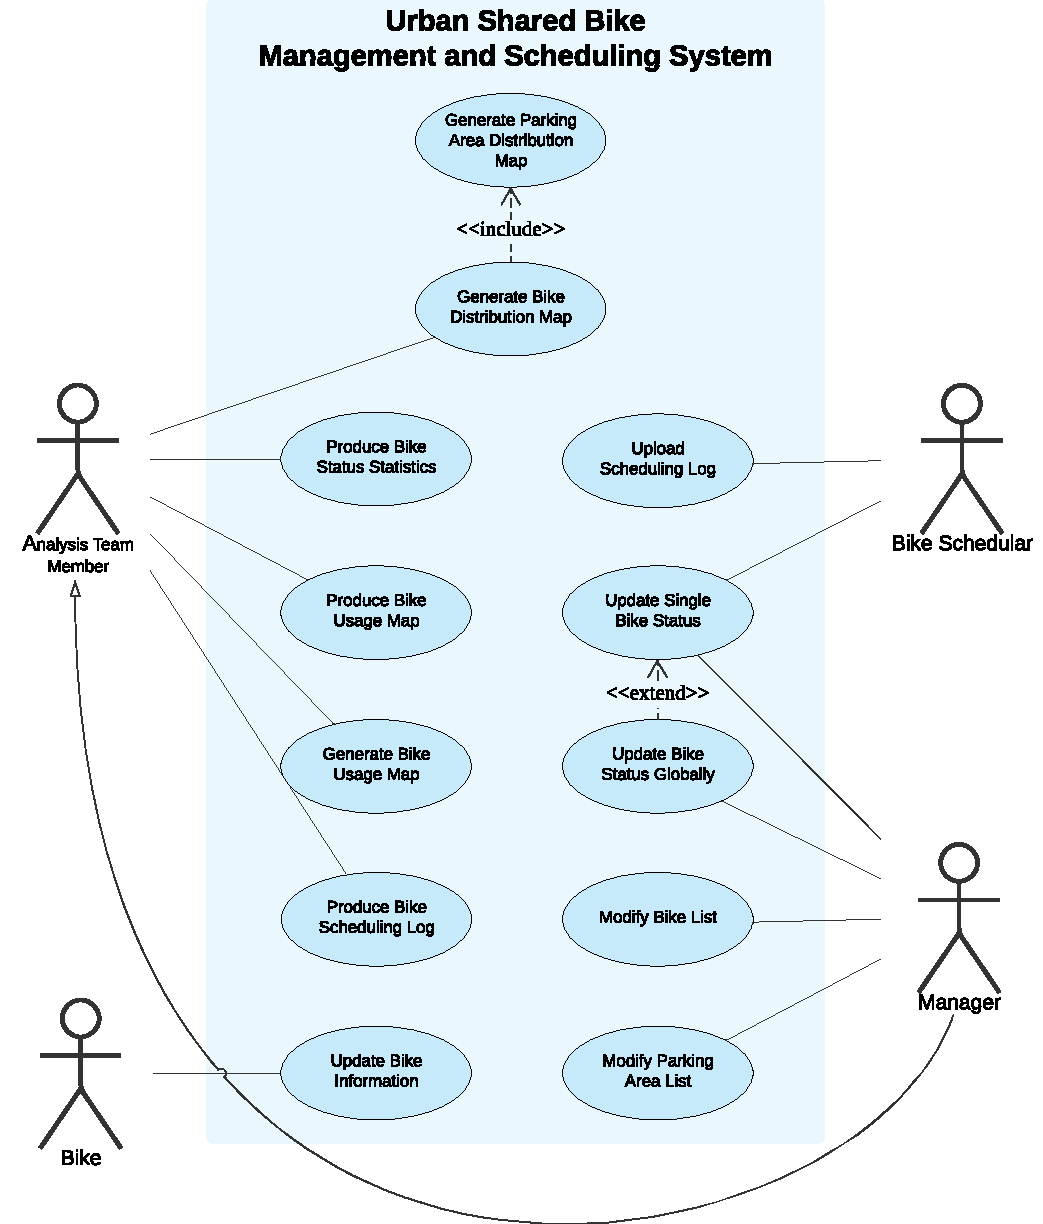
\includegraphics[width=0.99\textwidth]{figures/UseCase.pdf}
    \caption{用例汇总}\label{UseCase}
\end{figure}


\begin{figure}
    \centering
 \begin{mdframed}[leftmargin=0pt, rightmargin=0pt]
    \textbf{简要说明}

    用例\texttt{Generate Bike Distribution Map}使得分析团队成员和调度员能够查看共享单车的实时分布。

\noindent\rule{\textwidth}{0.5pt} % 实线分割线
    \textbf{分步说明}

    \begin{enumerate}
        \item 系统从数据库中收集所有共享单车的坐标及其状态;
        \item 系统依据单车坐标将单车标注在电子地图中;
        \item 系统依据单车坐标生成热力图;
        \item 系统通过用例\texttt{Generate Parking Area Distribution Map}在地图中标注停车区域;
        \item 系统调整地图窗口显示区域。
    \end{enumerate}
\end{mdframed}   
\caption{用例\texttt{Generate Bike Distribution Map}}\label{GenerateBikeDistributionMap}
\end{figure}

\begin{figure}
    \centering
 \begin{mdframed}[leftmargin=0pt, rightmargin=0pt]
    \textbf{简要说明}

    用例\texttt{Generate Parking Area Distribution Map}使得分析团队成员和调度员能够查看停车区域的分布情况。

\noindent\rule{\textwidth}{0.5pt} % 实线分割线
    \textbf{分步说明}

    \begin{enumerate}
        \item 系统从数据库中收集所有停车区域的中心坐标与半径;
        \item 系统利用中心坐标与半径在地图中绘制圆形区域以表示停车区域;
    \end{enumerate}
\end{mdframed}   
\caption{用例\texttt{Generate Parking Area Distribution Map}}\label{GenerateParkingAreaDistributionMap}
\end{figure}

\begin{figure}
    \centering
 \begin{mdframed}[leftmargin=0pt, rightmargin=0pt]
    \textbf{简要说明}

    用例\texttt{Upload Scheduling Log}使得调度员能够上传调度日志。

\noindent\rule{\textwidth}{0.5pt} % 实线分割线
    \textbf{分步说明}

    \begin{enumerate}
        \item 调度员通过API接口向系统上传调度日志;
        \item 系统将数据保存至\texttt{scheduling}表中;
    \end{enumerate}
\end{mdframed}   
\caption{用例\texttt{Upload Scheduling Log}}\label{UploadSchedulingLog}
\end{figure}



\begin{figure}
    \centering
 \begin{mdframed}[leftmargin=0pt, rightmargin=0pt]
    \textbf{简要说明}

    用例\texttt{Update Single Bike Status}使得调度员能够更新单个单车的状态。

\noindent\rule{\textwidth}{0.5pt} % 实线分割线
    \textbf{分步说明}

    \begin{enumerate}
        \item 调度员通过API接口向系统上传修改表单;
        \item 系统将修改表单保存至\texttt{to\_be\_reviewed\_status},\texttt{to\_be\_reviewed\_proof\_material}和\texttt{to\_be\_reviewed}中;
        \item 管理者审核表单;
        \item 若通过,则系统更新\texttt{bike\_status};否则,系统不对数据进行更新。
        \item 系统从\texttt{to\_be\_reviewed},\texttt{to\_be\_reviewed\_status}和\texttt{to\_be\_reviewed\_proof\_material}中删除相关数据;
    \end{enumerate}
\end{mdframed}   
\caption{用例\texttt{Update Single Bike Status}}\label{UpdateSingleBikeStatus}
\end{figure}

\begin{figure}
    \centering
 \begin{mdframed}[leftmargin=0pt, rightmargin=0pt]
    \textbf{简要说明}

    用例\texttt{Produce Bike Scheduling Log}使得分析团队成员能够获取单车的调度日志。

\noindent\rule{\textwidth}{0.5pt} % 实线分割线
    \textbf{分步说明}

    \begin{enumerate}
        \item 分析团队成员输入待查询单车的id号;
        \item 系统在\texttt{scheduling}表中查询与指定单车相关的调度信息;
        \item 系统按照时间顺序将调度信息进行整理,并利用\texttt{action}域进行配对;
        \item 系统打印整理后的调度信息。
    \end{enumerate}
\end{mdframed}   
\caption{用例\texttt{Produce Bike Scheduling Log}}\label{ProduceBikeSchedulingLog}
\end{figure}

\begin{figure}
    \centering
 \begin{mdframed}[leftmargin=0pt, rightmargin=0pt]
    \textbf{简要说明}

    用例\texttt{Generate Bike Usage Map}使得分析团队成员能够获取单车的使用情况时空分布。

\noindent\rule{\textwidth}{0.5pt} % 实线分割线
    \textbf{分步说明}

    \begin{enumerate}
        \item 分析团队成员选择查询时间段;
        \item 系统在\texttt{usage}表中查询所有单车在指定时间段内的使用情况;
        \item 系统将筛选得到的使用情况按照时间顺序进行整理,并利用\texttt{action}域进行配对;
        \item 系统将使用情况标记在电子地图中。
    \end{enumerate}
\end{mdframed}   
\caption{用例\texttt{Generate Bike Usage Map}}\label{GenerateBikeUsageMap}
\end{figure}

\begin{figure}
    \centering
 \begin{mdframed}[leftmargin=0pt, rightmargin=0pt]
    \textbf{简要说明}

    用例\texttt{Produce Bike Status Statistics}使得分析团队成员能够获取单车的状态统计信息。

\noindent\rule{\textwidth}{0.5pt} % 实线分割线
    \textbf{分步说明}

    \begin{enumerate}
        \item 系统通过\texttt{bike\_status}表统计处于各状态的单车比例;
        \item 系统打印状态统计信息。
    \end{enumerate}
\end{mdframed}   
\caption{用例\texttt{Produce Bike Status Statistics}}\label{ProduceBikeStatusStatistics}
\end{figure}

\begin{figure}
    \centering
 \begin{mdframed}[leftmargin=0pt, rightmargin=0pt]
    \textbf{简要说明}

    用例\texttt{Update Bike Information}使得单车能够上传当前车辆信息。

\noindent\rule{\textwidth}{0.5pt} % 实线分割线
    \textbf{分步说明}

    \begin{enumerate}
        \item 单车通过API接口向系统上传位置、电池电量信息以及触发动作(开锁或关锁);
        \item 系统根据数据更新\texttt{bike}表;
        \item 系统根据\texttt{parking\_area}中的数据来判断是否需要更新单车状态。
    \end{enumerate}
\end{mdframed}   
\caption{用例\texttt{Update Bike Information}}\label{UpdateBikeInformation}
\end{figure}

\begin{figure}
    \centering
 \begin{mdframed}[leftmargin=0pt, rightmargin=0pt]
    \textbf{简要说明}

    用例\texttt{Update Bike Status Globally}使得管理者能够批量更新单车状态。

\noindent\rule{\textwidth}{0.5pt} % 实线分割线
    \textbf{分步说明}

    \begin{enumerate}
        \item 管理者在系统中确定状态更新的条件;
        \item 如果更新“低电量”状态,则系统根据\texttt{bike}表中的\texttt{battery\_remaining\_capacity}进行更新;
        \item 如果更新“闲置”状态,则系统根据\texttt{usage}表中的数据来获取各单车最近的关锁时间,依据此进行更新;
        \item 如果更新“长期未关锁”状态,则系统根据\texttt{usage}表中的数据来获取各单车最近的没有对应关锁行动的开锁行动,依据此进行更新;
        \item 如果更新“型号老旧”状态,则系统根据\texttt{bike}中的\texttt{production\_date}域来进行更新。
    \end{enumerate}
\end{mdframed}   
\caption{用例\texttt{Update Bike Status Globally}}\label{UpdateBikeStatusGlobally}
\end{figure}

\begin{figure}
    \centering
 \begin{mdframed}[leftmargin=0pt, rightmargin=0pt]
    \textbf{简要说明}

    用例\texttt{Modify Bike List}使得管理者能够添加或删除单车信息。

\noindent\rule{\textwidth}{0.5pt} % 实线分割线
    \textbf{分步说明}

    \begin{enumerate}
        \item 若管理者要求添加单车信息,则:
        \begin{enumerate}
            \item 管理者填写单车信息;
            \item 系统向\texttt{bike}表中插入该信息;
            \item 系统更新\texttt{contain}表。
        \end{enumerate}
        \item 若管理者要求删除单车信息,则:
        \begin{enumerate}
            \item 管理者输入待删除单车id;
            \item 系统在数据库中删除指定单车的相关信息。
        \end{enumerate}
    \end{enumerate}
\end{mdframed}   
\caption{用例\texttt{Modify Bike List}}\label{ModifyBikeList}
\end{figure}

\begin{figure}
    \centering
 \begin{mdframed}[leftmargin=0pt, rightmargin=0pt]
    \textbf{简要说明}

    用例\texttt{Modify Parking Area List}使得管理者能够添加或删除停车区域信息。

\noindent\rule{\textwidth}{0.5pt} % 实线分割线
    \textbf{分步说明}

    \begin{enumerate}
        \item 若管理者要求添加停车区域信息,则:
        \begin{enumerate}
            \item 管理者填写停车区域信息;
            \item 系统向\texttt{parking\_area}表中插入该信息;
            \item 系统更新\texttt{contain}表。
        \end{enumerate}
        \item 若管理者要求删除停车区域信息,则:
        \begin{enumerate}
            \item 管理者输入待删除停车区域id;
            \item 系统在数据库中删除指定停车区域的相关信息。
        \end{enumerate}
    \end{enumerate}
\end{mdframed}   
\caption{用例\texttt{Modify Parking Area List}}\label{ModifyParkingAreaList}
\end{figure}

\section{数据字典}
数据字典如表\ref{DataDictionary1}-\ref{DataDictionary3}所示。
\begin{table}
\centering
\caption{数据字典(调度相关部分)}
\label{DataDictionary1}
\begin{tabular}{lll}\toprule
  数据元素名称&描述&备注\\\midrule
scheduling log            &
   \makecell[l]{
    该数据元素包含以下域:\\
    \quad 坐标\\
    \quad 时间\\
    \quad 动作\\
    }                &\makecell[l]{坐标由经纬度构成;\\动作为“开始”或“结束”}              \\
scheduling history&与scheduling log包含相同的域&数据库中存储的所有调度记录\\
required scheduling history&与scheduling log包含相同的域&指定单车的历史调度记录\\
 \bottomrule
\end{tabular}
\end{table}

\begin{table}
\centering
\caption{数据字典(停车区域相关部分)}
\label{DataDictionary2}
\begin{tabular}{lll}\toprule
  数据元素名称&描述&备注\\\midrule
parking area info          &   \makecell[l]{
    该数据元素包含以下域:\\
    \quad 停车区域名称\\
    \quad 停车区域坐标\\
    \quad 停车区域半径\\
    }                &\makecell[l]{坐标由经纬度构成;\\半径单位为米}             \\
 \bottomrule
\end{tabular}
\end{table}

\begin{table}
\centering
\caption{数据字典(审核相关部分)}
\label{DataDictionary3}
\begin{tabular}{lll}\toprule
  数据元素名称&描述&备注\\\midrule
change form                         &  \makecell[l]{
    该数据元素包含以下域:\\
    \quad 单车id\\
    \quad 更新后的单车状态\\
    \quad 证明材料\\
    }&\makecell[l]{证明材料为图片}    \\
comment                    &0或1             &  \makecell[l]{为1代表通过,\\否则拒绝单车状态更改生效}    \\
Review                     &\makecell[l]{输入参数:\\\quad 待改变状态\\\quad 支撑材料\\输出参数:\\\quad 审核意见}&\makecell[l]{
    该流程的步骤为:\\
    \quad 管理者查看待更改状态和相应的图片\\
    \quad 管理者作出审核意见\\
    }          \\
 \bottomrule
\end{tabular}
\end{table}
\begin{longtable}{lll}
    \caption{数据字典(单车相关部分)}\label{DataDictionary4} \\
    \toprule
  数据元素名称&描述&备注\\
  \midrule
  \endfirsthead
    \toprule
  数据元素名称&描述&备注\\
  \midrule
  \endhead

  \midrule
\multicolumn{3}{r}{表格继续下一页} \\
\bottomrule
\endfoot

% 设置表格最后一页的表尾内容
\bottomrule
\endlastfoot

bike status       &    \makecell[l]{
    取值范围如下:\\
    \quad 正常\\
    \quad 违规停放\\
    \quad 低电量\\
    \quad 闲置\\
    \quad 长期未关锁\\
    \quad 异常\\
    \quad 待维修\\
    \quad 型号老旧\\
    \quad 入库\\
    }         &\makecell[l]{ 描述单车当前状态,\\可由多个状态合理组合而成 }\\
updated bike status               & 与bike status一致                 &描述更新后的单车状态    \\
bike info                         &  \makecell[l]{
    该数据元素包含以下域:\\
    \quad 单车id\\
    \quad 单车坐标\\
    \quad 单车生产日期\\
    }&\makecell[l]{用于初始化单车数据\\单车生产日期格式为YYYY:MM:DD}    \\
uploaded data                         &  \makecell[l]{
    该数据元素包含以下域:\\
    \quad 单车id\\
    \quad 单车坐标\\
    \quad 单车剩余电量\\
    \quad 行动\\
    }&\makecell[l]{由单车上传的信息\\行动为1代表是开锁动作,\\为0代表是关锁动作 }    \\
previous status                         &  \makecell[l]{
    该数据元素包含以下域:\\
    \quad 单车状态\\
    \quad 最近使用时间\\
    }&用于和待更新状态进行对比 \\
map data                         &  \makecell[l]{
    该数据元素包含以下域:\\
    \quad 单车id\\
    \quad 单车状态\\
    \quad 单车坐标\\
    }&用于绘制单车分布图 \\
usage data                         &  \makecell[l]{
    该数据元素包含以下域:\\
    \quad 单车id\\
    \quad 起始坐标\\
    \quad 起始时间\\
    \quad 结束坐标\\
    \quad 结束时间\\
    }&用于绘制单车使用情况时空图 \\
uploaded usage data                         &  \makecell[l]{
    该数据元素包含以下域:\\
    \quad 单车id\\
    \quad 单车坐标\\
    \quad 行动时间\\
    \quad 行动\\
    }&\makecell[l]{由单车上传的信息\\行动为1代表是开锁动作,\\为0代表是关锁动作 } \\
bike status statistics     &处于各状态的单车数量占总数的比例          &  格式为**.**\%            \\
time period                &指定时间段          &  用于生成单车使用情况分布图            \\
uploaded bike info                         &  \makecell[l]{
    该数据元素包含以下域:\\
    \quad 单车坐标\\
    \quad 剩余电量\\
    \quad 状态更新\\
    }&\makecell[l]{依据单车坐标和剩余电量更新状态 } \\

\end{longtable}


\section{数据流图}
数据流图如图\ref{DataFlow}所示。

除过程Review外,数据流图中的其余过程已在图\ref{GenerateBikeDistributionMap}-\ref{ModifyParkingAreaList}中以用例的形式来描述,所以不在数据字典中重复,
其中流程Update Bike Status对应于用例\texttt{Update Bike Status Globally}和\texttt{Update Single Bike Status}外,其余流程都对应于其同名用例。

\begin{figure}[!htbp]
    \centering
    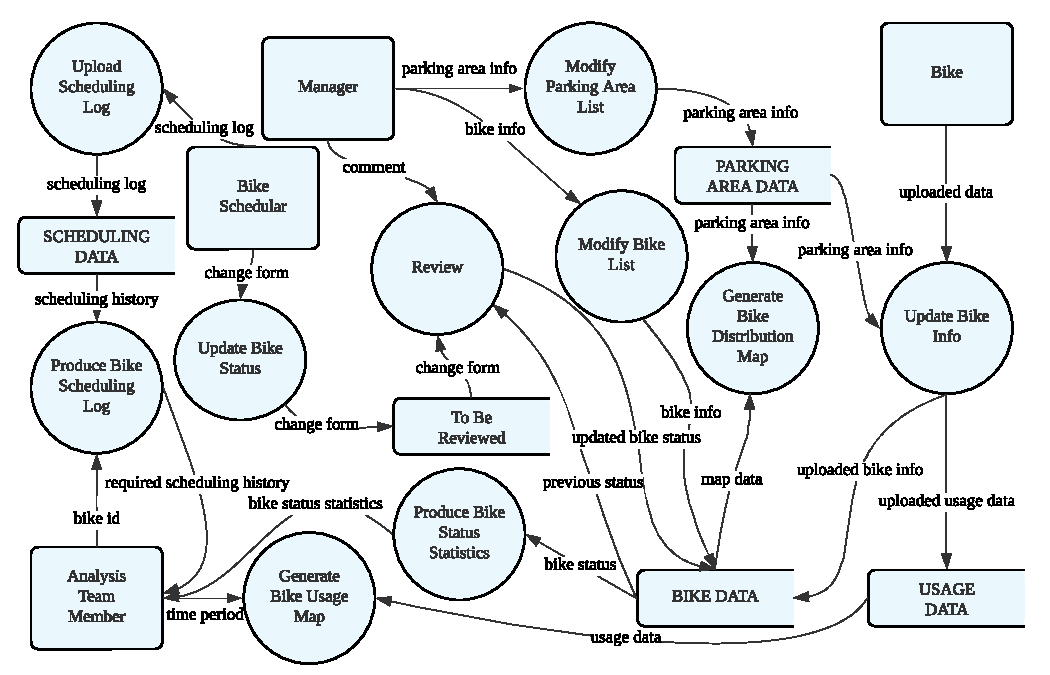
\includegraphics[width=\textwidth]{figures/DataFlow.pdf}
    \caption{数据流图}\label{DataFlow}
\end{figure}

\section{整体设计}
\subsection{数据库设计}

本系统采用分层的数据架构设计,包括数据处理层和规范化数据层两个层次:
\begin{enumerate}
  \item 数据处理层
  \begin{itemize}
    \item 目的:支持数据采集和清洗的ETL过程
    \item 特点:
    \begin{itemize}
      \item 保留原始数据格式,便于追溯和验证
      \item 允许数据冗余,不强制遵循3NF
      \item 支持增量更新和批量处理
    \end{itemize}
    \item 组成:
    \begin{itemize}
      \item 原始数据表:分别存储BOSS直聘和猎聘网的原始爬虫数据
      \item 暂存数据表:存储统一格式和质量检查后的中间数据
    \end{itemize}
  \end{itemize}

  \item 规范化数据层
  \begin{itemize}
    \item 目的:
    \begin{itemize}
      \item 提供高质量的规范化数据
      \item 支持复杂的数据查询和分析
      \item 保证数据一致性
    \end{itemize}
    \item 特点:
    \begin{itemize}
      \item 严格遵循3NF,消除数据冗余
      \item 建立完整的实体关系
      \item 支持事务处理
    \end{itemize}
    \item 组成:
    \begin{itemize}
      \item 基础实体表:包含用户、公司、职位、地址四个核心实体
      \item 关联关系表:维护实体间的多对多关系
      \item 物化视图:预计算常用查询结果,提升查询性能
    \end{itemize}
  \end{itemize}
\end{enumerate}

\begin{figure}[htbp]
  \centering
  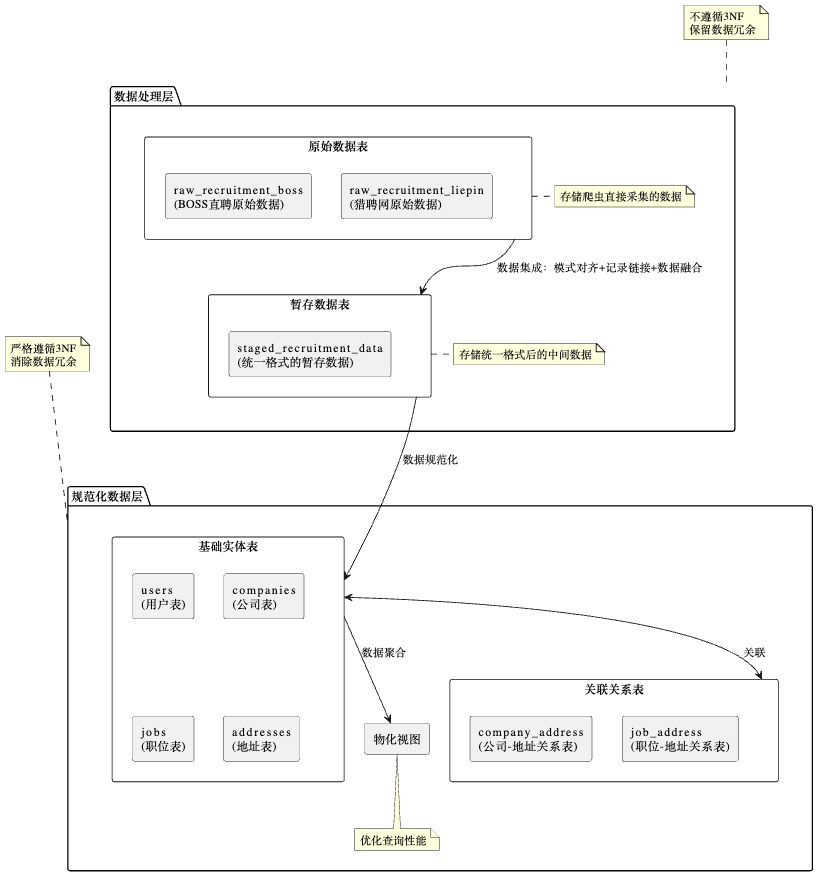
\includegraphics[width=0.8\textwidth]{figures/数据库概念设计.png}
  \caption{系统数据架构图}
  \label{fig:data_architecture}
\end{figure}


数据库采用分层架构设计,分为数据处理层和规范化数据层。这种分层设计有效分离了数据采集处理和业务数据存储的职责,使系统具有更好的可维护性和扩展性。

\subsubsection{数据处理层}
数据处理层不严格遵循第三范式,保留适度的数据冗余以支持数据处理和追溯。该层包含原始数据表和暂存数据表两类重要组件。原始数据表分别存储来自BOSS直聘和猎聘网的爬虫采集数据,完整保留了JSON格式的原始数据,并通过processed字段标记处理状态,支持数据的增量处理和历史追溯。

暂存数据表则作为数据集成的中间层,承担着数据规范化的重要职责。它通过统一的字段命名和格式规范,实现了不同来源数据的模式对齐。同时,暂存表还包含了一系列特殊设计字段,如record\_hash\_for\_linkage和duplicate\_group\_id用于数据去重,is\_master\_record和linked\_record\_ids用于关联记录管理,这些设计为后续的记录链接和数据融合提供了基础支持。

数据处理层的实体之间形成了清晰的数据流转路径:

\begin{itemize}
    \item 数据采集阶段:
    \begin{itemize}
        \item 爬虫程序分别从BOSS直聘和猎聘网采集数据
        \item 原始数据分别存入对应的原始数据表
        \item 通过processed字段标记数据的处理状态
    \end{itemize}
    
    \item 数据清洗阶段:
    \begin{itemize}
        \item 原始数据经过清洗后存入暂存数据表
        \item 统一数据格式,规范字段命名
        \item 进行数据去重和关联处理
    \end{itemize}
    
    \item 数据转换阶段:
    \begin{itemize}
        \item 暂存数据经过规范化处理
        \item 通过record\_hash\_for\_linkage进行重复检查
        \item 使用duplicate\_group\_id管理重复记录组
        \item 通过is\_master\_record标记主记录
    \end{itemize}
\end{itemize}

这种分层的数据处理设计确保了数据的可追溯性和处理过程的可控性,同时通过合理的字段设计,保证了数据处理的效率和准确性。

\subsubsection{规范化数据层}
规范化数据层严格遵循第三范式设计原则,通过消除数据冗余来保证数据一致性。该层主要由基础实体表、关联关系表和物化视图三部分构成。基础实体表包括用户、公司、职位和地址四个核心实体,每个实体表都独立管理其特有属性。关联关系表(company\_address和job\_address)则专门处理实体间的多对多关系,通过外键约束确保数据完整性。

为了平衡规范化设计带来的查询性能影响,该层还包含了物化视图组件。物化视图通过预先计算和存储常用查询结果,在保证数据一致性的同时提供了优秀的查询性能。这种设计既保持了规范化的优势,又解决了实际应用中的性能需求。

两个数据层之间通过明确的数据流向连接:原始数据经过清洗和转换进入暂存表,再经过规范化处理后存入实体表和关系表,最后通过物化视图提供高效的数据服务。这种渐进式的数据处理流程,确保了数据质量的同时,也保证了整个过程的可控性和可追溯性。

如图\ref{fig:data_architecture}所示,系统采用分层架构设计,将数据处理层和规范化数据层进行清晰分离。数据处理层包含BOSS直聘(raw\_recruitment\_boss)和猎聘网(raw\_recruitment\_liepin)的原始数据表,以及用于存储统一格式数据的暂存表(staged\_recruitment\_data),不严格遵循第三范式以支持数据处理和追溯。规范化数据层则严格遵循3NF范式,由用户(users)、公司(companies)、职位(jobs)、地址(addresses)四个基础实体表,以及公司-地址(company\_address)、职位-地址(job\_address)两个关联关系表组成,并通过物化视图(recruitment\_mv)优化查询性能。数据流向是从原始数据经过清洗后存入暂存表,再经规范化处理后存入实体表和关系表,最后通过物化视图提供高效的数据查询服务。


\subsection{后端设计}

在设计本系统时,面临着多个关键挑战:首先是需要处理来自不同招聘网站的异构数据,这些数据格式和结构各不相同;其次是需要确保数据的实时性和准确性,因为招聘信息经常会发生变化;最后是需要提供高效的数据查询和分析功能,以支持各种数据可视化和统计分析需求。

为了应对这些挑战,采用了分层架构设计,通过清晰的数据流向和模块划分,实现了从数据采集到数据展示的完整流程。如图\ref{fig:system_dataflow_simplified}所示,系统主要包含六个核心层次:外部数据源层、ETL处理层、数据存储层、CRUD层、API服务层和后台服务层。这种分层设计不仅使系统结构清晰,便于维护和扩展,还能够有效地隔离不同功能模块,提高系统的可靠性和可维护性。

\begin{figure}[htbp]
    \centering
    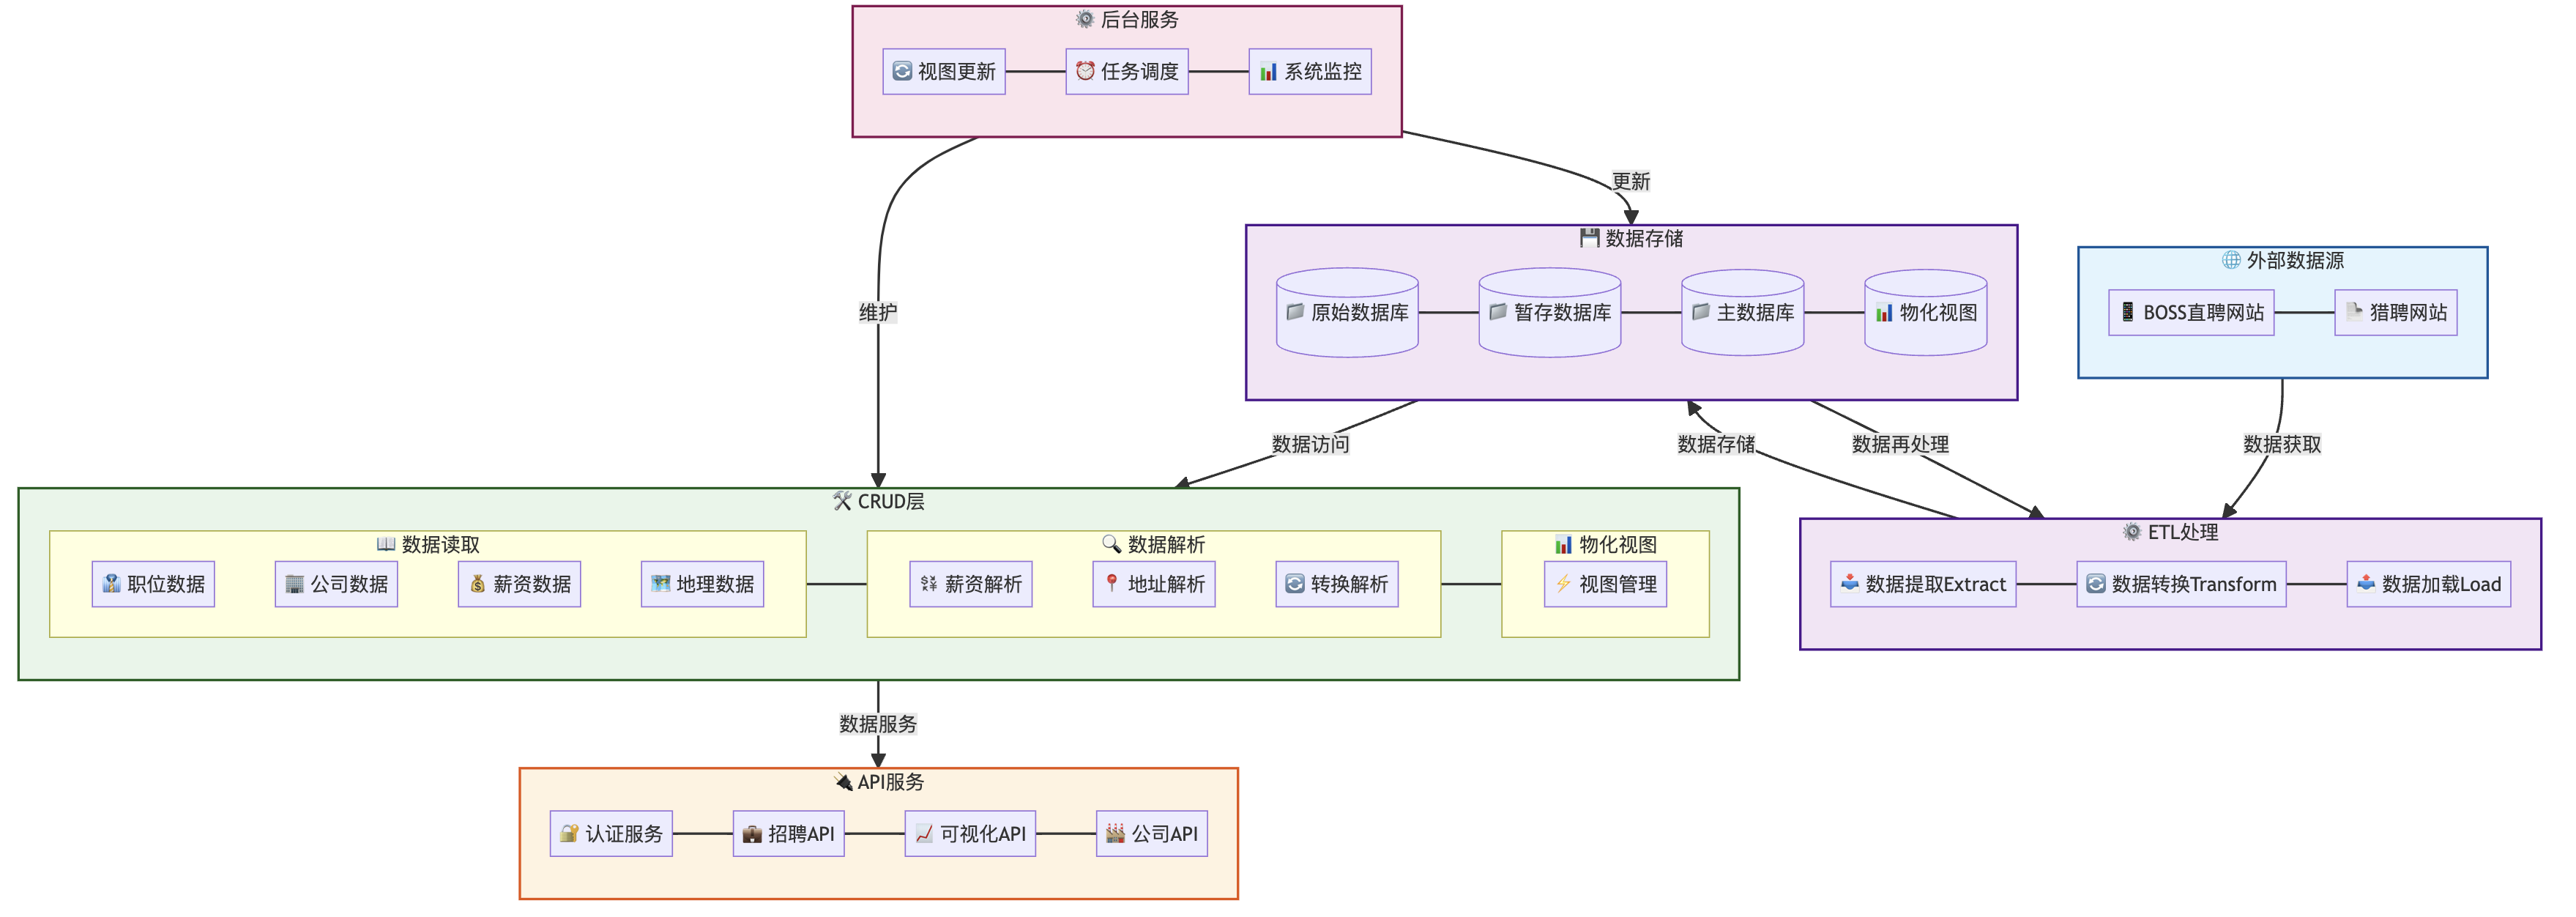
\includegraphics[width=1.0\textwidth]{figures/系统数据流图简化版.png}
    \caption{系统数据流图简化版}
    \label{fig:system_dataflow_simplified}
\end{figure}



图\ref{fig:system_dataflow}是系统数据流图的详细版本,展示了系统从数据采集到数据展示的完整流程。该图通过流程图的形式详细展示了系统的数据流向:从BOSS直聘和猎聘网站的数据源开始,数据首先经过ETL处理层的提取、转换和加载三个阶段,然后依次存储在原始数据库、暂存数据库、主数据库和物化视图中。CRUD层负责数据的基础操作,包括职位、公司、薪资和地理数据的读取与解析,以及物化视图的管理。API服务层则提供了认证、招聘信息、可视化和公司信息等对外接口。整个系统由后台服务层的任务调度器进行统一调度,通过物化视图更新服务保持数据的实时性,并通过系统监控确保各个模块的正常运行。这种层次分明的架构设计不仅确保了数据处理的完整性和可靠性,也为系统的扩展和维护提供了便利。

\begin{figure}[htbp]
    \centering
    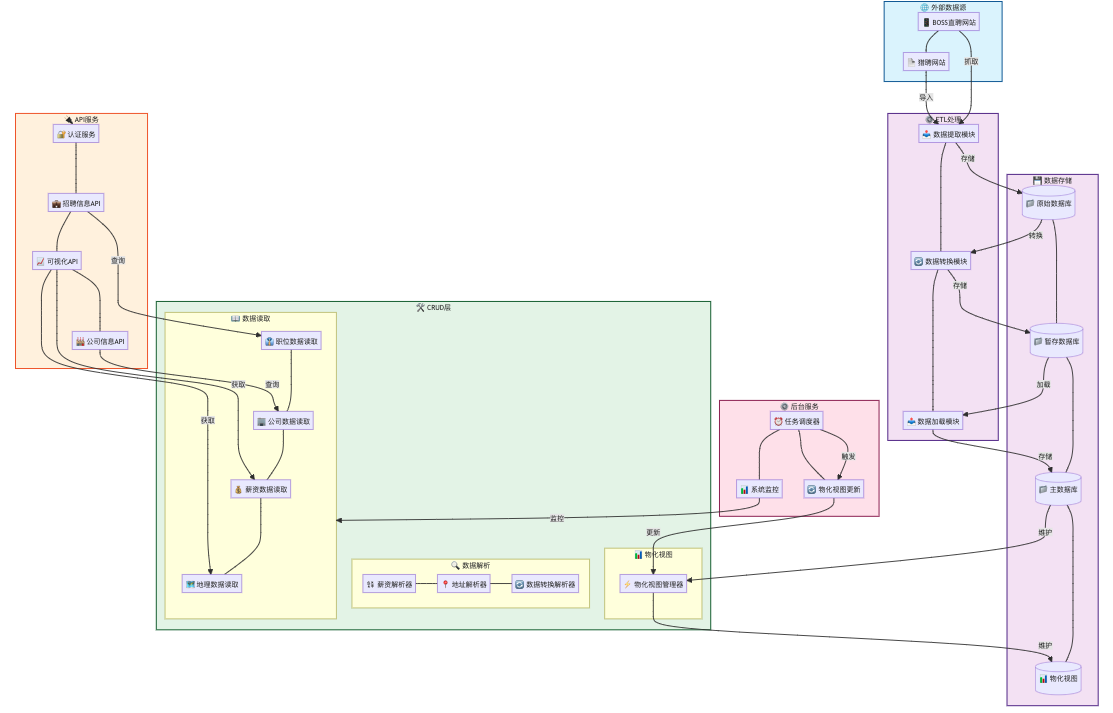
\includegraphics[width=1.0\textwidth]{figures/系统数据流图.png}
    \caption{系统数据流图}
    \label{fig:system_dataflow}
\end{figure}

\subsection{数据集成}
本系统实现了一个完整的ETL(Extract-Transform-Load)数据集成流程,将来自不同招聘网站的职位数据进行整合、清洗和标准化,最终加载到规范化的数据库中。整个过程包括数据抽取(Extract)、数据转换(Transform)和数据加载(Load)三个主要阶段。如图\ref{fig:ETL1}所示。

\begin{figure}[htbp]
    \centering
    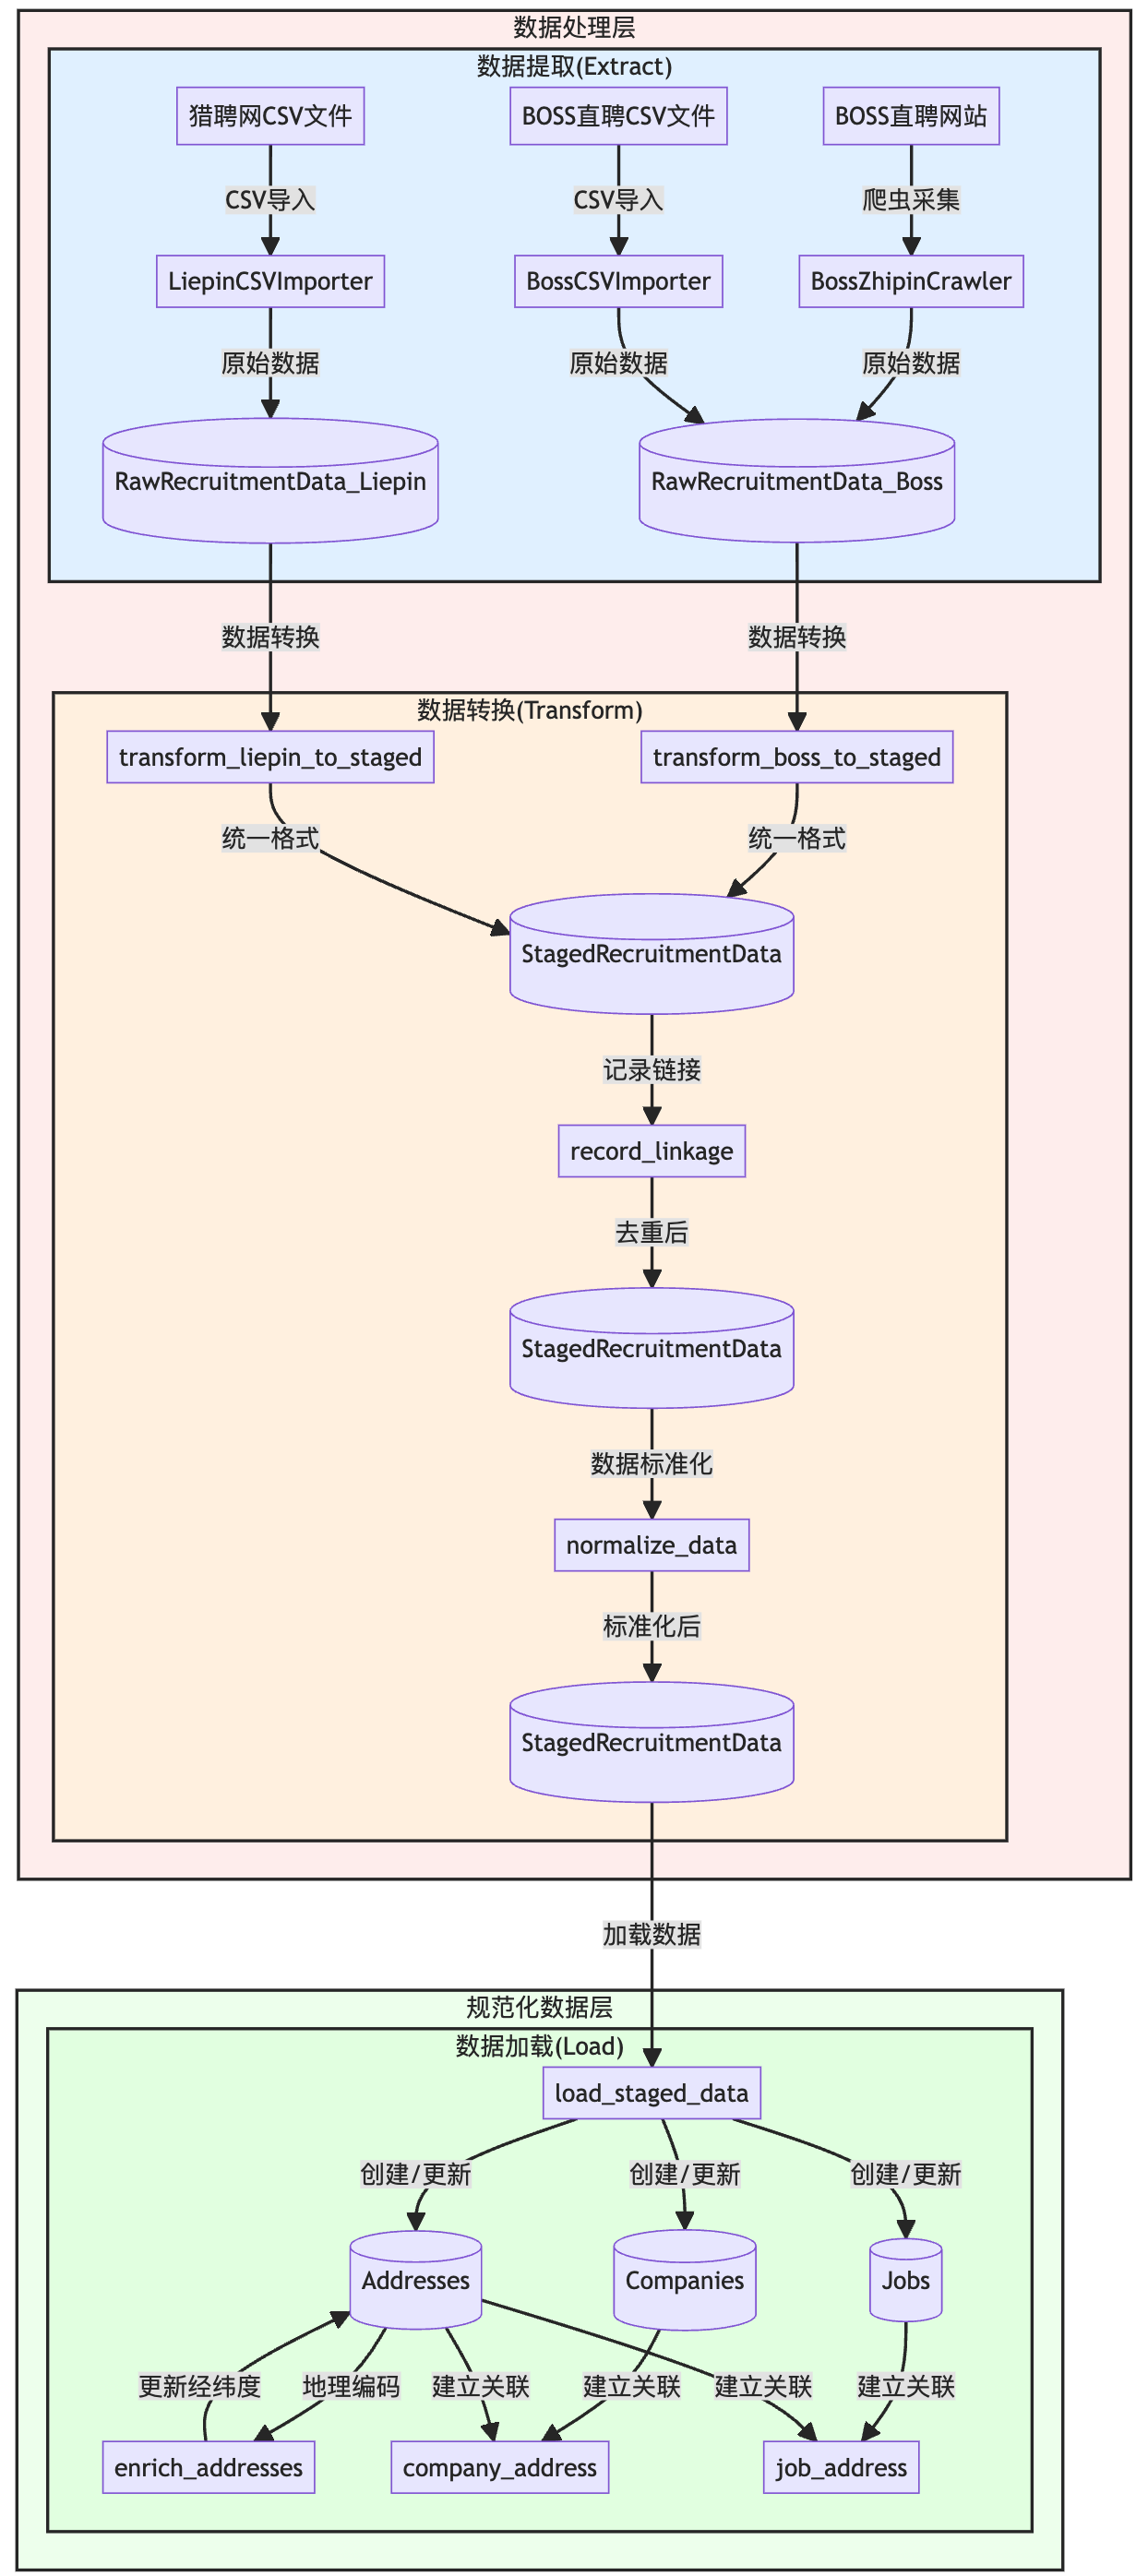
\includegraphics[width=0.6\textwidth]{figures/ETL.png}
    \caption{ETL数据集成流程}
    \label{fig:ETL1}
\end{figure}

\subsection{API实现}

系统的API层采用FastAPI框架实现,遵循RESTful架构设计原则,提供了一系列标准化的HTTP接口。

\subsection{前端设计}
本项目的前端采用Next.js框架,使用React和NextUI来构建页面和组件,使用Tailwind CSS进行样式设计。
特别地,我们采用Next.js最新推出的文件路由系统,将文件组织结构自动映射到网页路由。

前端通过API来获取后端通过Plotly生成的网页元素,并将其进行渲染。
\section{详细设计}
\subsection{数据库设计}

\subsubsection{实体定义}
规范化数据层包含用户(User)、公司(Company)、职位(Job)和地址(Address)四个核心实体。这些实体严格遵循第三范式设计,消除数据冗余,保证数据一致性。用户实体用于系统访问控制,支持普通用户和管理员两种角色,确保系统安全;公司实体规范化存储招聘企业的基本信息,通过唯一的公司名称避免重复;职位实体以标准化格式记录招聘信息,通过外键关联到发布公司;地址实体则规范化存储地理位置信息,支持地理空间查询。实体之间通过关联关系表维护多对多关系,形成完整且规范的数据模型。表\ref{tab:entity_definition}详细说明了规范化数据层各实体的定义:

\begin{table}[htbp]
  \centering
  \caption{系统实体定义}
  \label{tab:entity_definition}
  \begin{tabular}{|p{0.15\textwidth}|p{0.35\textwidth}|p{0.4\textwidth}|}
    \hline
    \begin{center}\textbf{实体名称}\end{center} & \begin{center}\textbf{主要属性}\end{center} & \begin{center}\textbf{说明}\end{center} \\
    \hline
    \multirow{5}{*}{用户(User)} & 
    \begin{itemize}
      \item 用户ID(主键)
      \item 用户名
      \item 密码
      \item 用户角色
      \item 创建时间
    \end{itemize} & 
    \begin{center}系统用户信息,支持基本的角色权限控制。用户可以分为普通用户和管理员两种角色,用于管理系统访问权限。\end{center} \\
    \hline
    \multirow{6}{*}{公司(Company)} & 
    \begin{itemize}
      \item 公司ID(主键)
      \item 公司名称(唯一)
      \item 所属行业
      \item 公司规模
      \item 创建时间
      \item 更新时间
    \end{itemize} & 
    \begin{center}招聘公司的基本信息。公司名称需要保持唯一性以避免重复,通过所属行业和公司规模等属性可以支持多维度的分析查询。\end{center} \\
    \hline
    \multirow{11}{*}{职位(Job)} & 
    \begin{itemize}
      \item 职位ID(主键)
      \item 职位名称
      \item 职位类型
      \item 薪资范围
      \item 经验要求
      \item 学历要求
      \item 技能要求
      \item 职位福利
      \item 数据来源
      \item 创建时间
      \item 更新时间
    \end{itemize} & 
    \begin{center}职位发布的详细信息。包含职位要求、待遇等完整招聘信息,通过数据来源字段可以追踪数据来源渠道。\end{center} \\
    \hline
    \multirow{6}{*}{地址(Address)} & 
    \begin{itemize}
      \item 地址ID(主键)
      \item 地址文本
      \item 经度
      \item 纬度
      \item 创建时间
      \item 更新时间
    \end{itemize} & 
    \begin{center}公司和职位关联的地理位置信息。通过经纬度坐标支持地理位置检索和距离计算,可用于就近推荐等功能。\end{center} \\
    \hline
  \end{tabular}
\end{table}

图\ref{fig:normalized_data_er}展示了规范化数据层的数据结构设计。该设计严格遵循第三范式(3NF),通过实体表和关系表的合理组织,消除了数据冗余,保证了数据一致性。该E-R图清晰地展示了系统中各实体之间的关联关系,为后续的物理设计和系统实现提供了重要指导。下面是关于图中的实体表User、Company、Job和Address和关系表company\_address、job\_address的详细说明。

\begin{figure}[htbp]
  \centering
  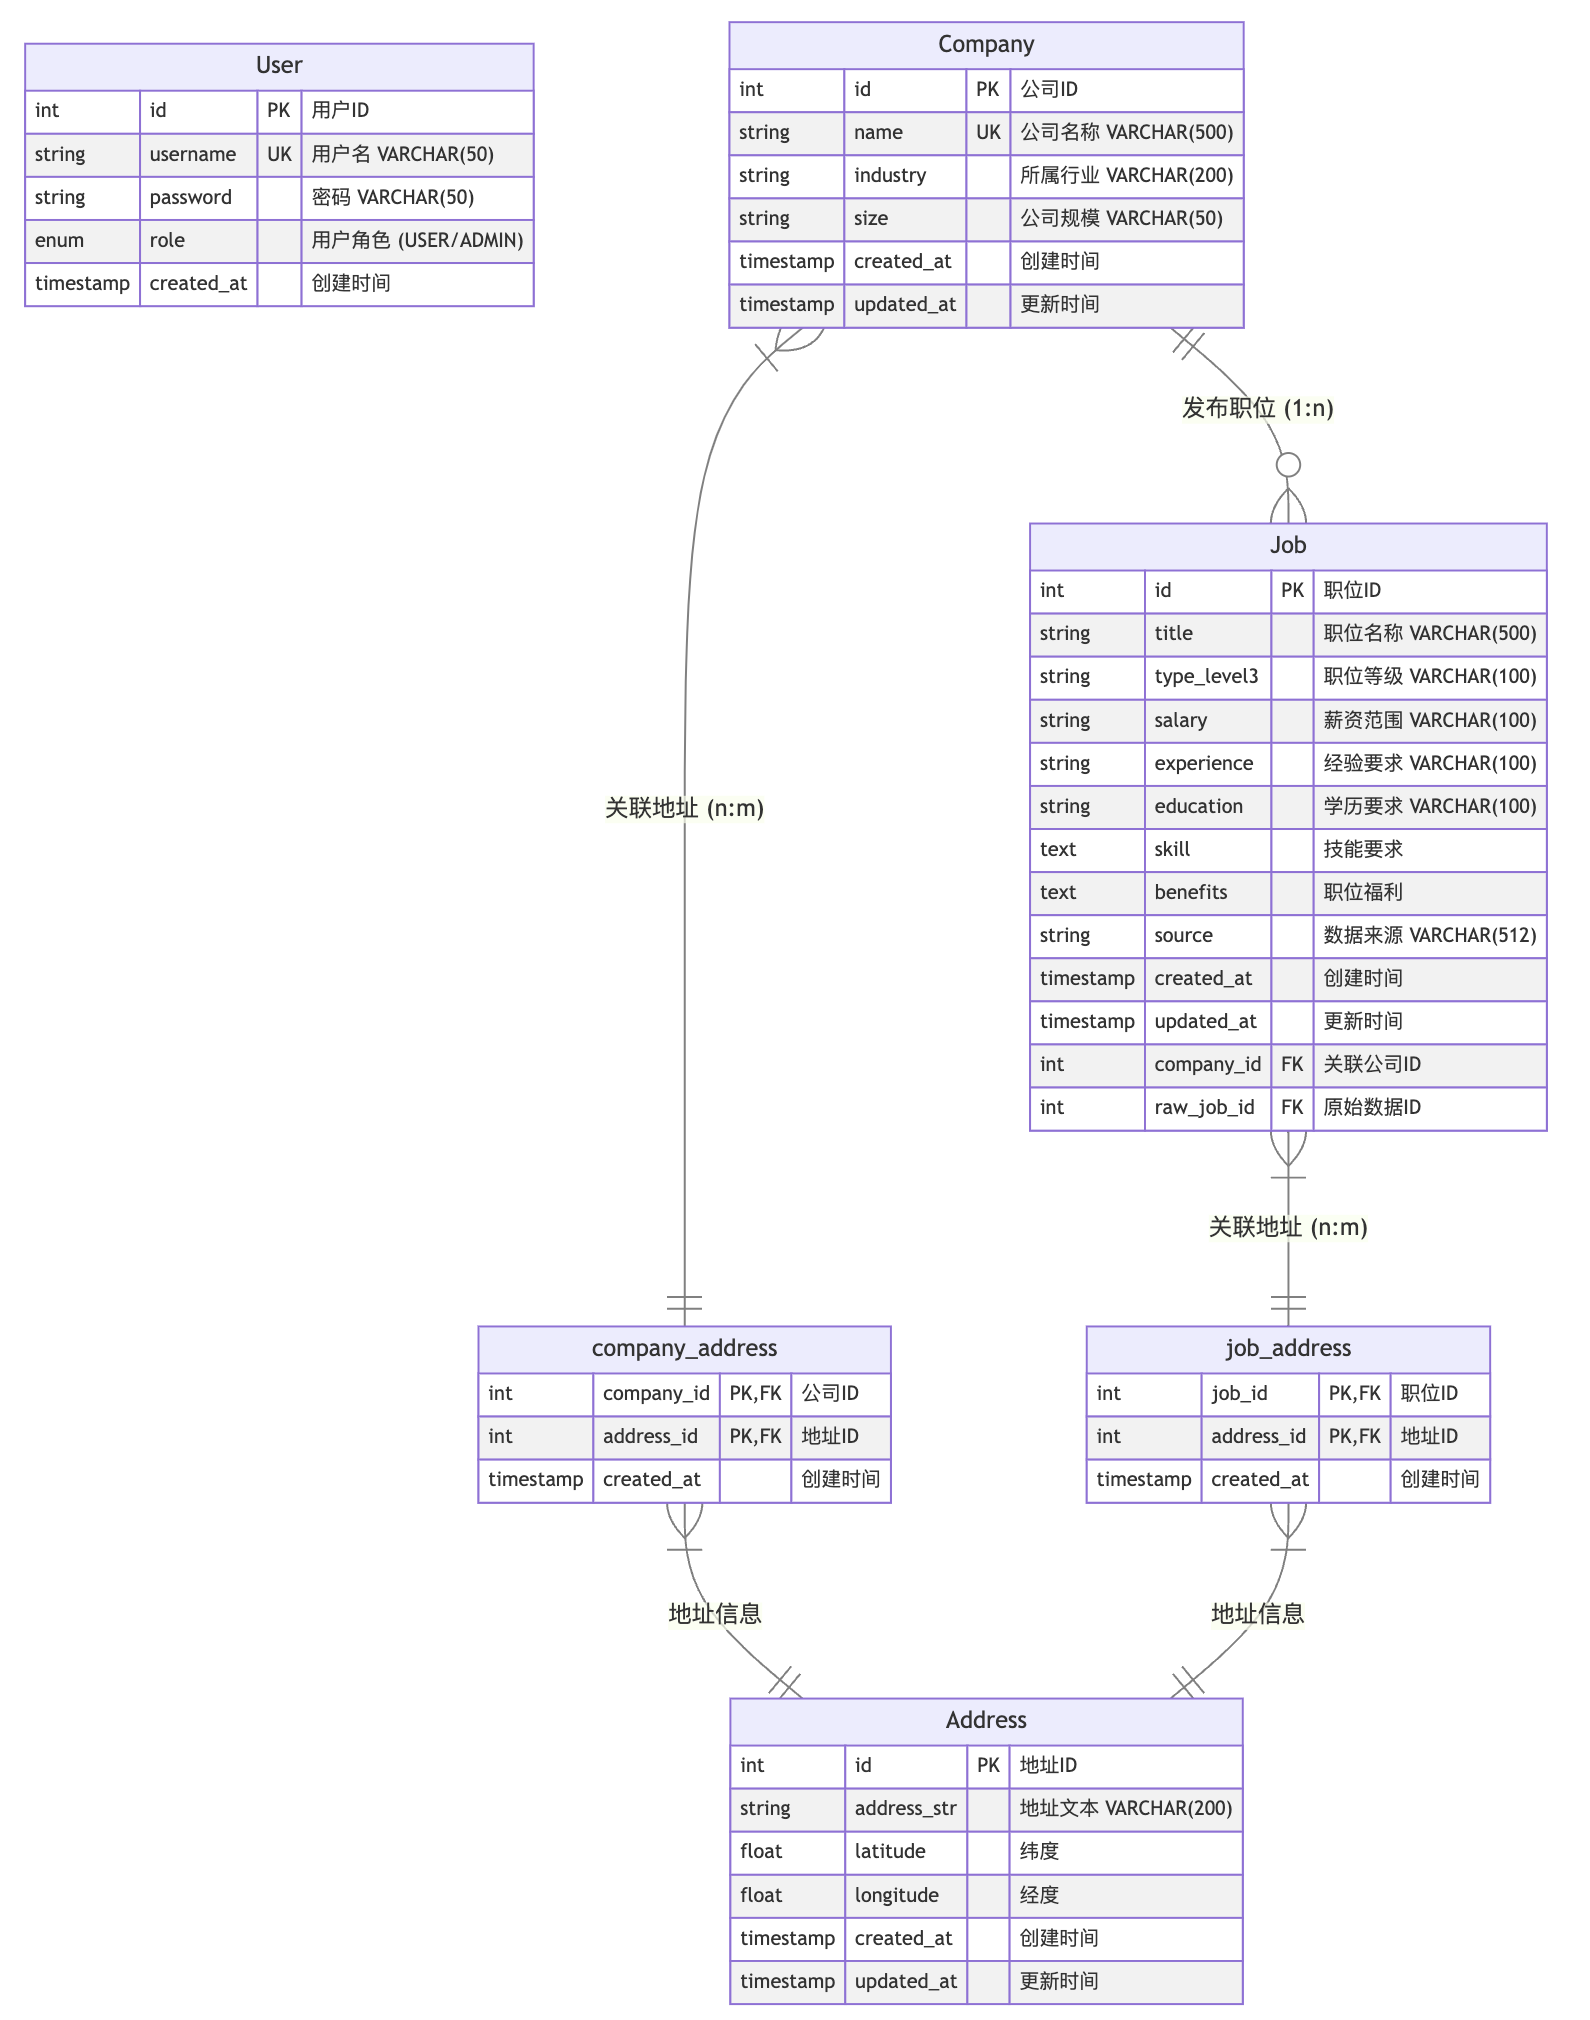
\includegraphics[width=0.8\textwidth]{figures/数据库实体ER图.png}
  \caption{规范化数据层E-R图}
  \label{fig:normalized_data_er}
\end{figure}


\paragraph{核心实体表设计}
系统的数据模型主要由四个基本实体表构成,每个实体表都严格遵循第三范式(3NF)设计原则。用户(User)表作为系统的基础用户管理单元,存储用户的身份认证和授权信息。该表包含用户ID作为主键,用户名设置唯一约束,同时存储密码和用户角色信息。通过角色字段(枚举类型:user/admin)实现基本的权限管理,并在用户名上建立索引(ix\_users\_username)以优化登录查询性能。

公司(Company)表存储招聘公司的核心信息,是职位信息的关联主体。该表以公司ID为主键,公司名称设置唯一约束,同时包含所属行业、公司规模等基本信息字段。为支持多维度的查询需求,表中建立了针对性的复合索引,包括公司名称索引(ix\_companies\_name)、行业规模复合索引(ix\_companies\_industry\_size)以及名称行业复合索引(ix\_companies\_name\_industry)。

职位(Job)表作为系统的核心业务实体,存储完整的招聘信息。除职位ID主键外,该表包含职位名称、类型、薪资范围、经验要求、学历要求等详细信息。通过company\_id外键与公司表建立关联,实现一对多关系,同时通过raw\_job\_id关联到暂存数据表保证数据可追溯性。该表设计了多个针对性索引,包括职位名称索引(ix\_jobs\_title)、公司关联索引(ix\_jobs\_company\_id)等,以优化不同场景下的查询性能。

地址(Address)表统一管理地理位置信息,支持地理空间查询功能。该表包含地址ID主键、地址文本、经纬度坐标等字段。特别值得注意的是,该表使用了PostgreSQL的GIN索引(ix\_addresses\_address\_str\_trgm)支持地址文本的模糊查询,并通过经纬度复合索引(ix\_addresses\_coordinates)支持地理位置检索和距离计算。

\paragraph{关系表设计}
为处理实体间的多对多关系,系统设计了两个关系表。公司-地址关联表(company\_address)通过复合主键(company\_id, address\_id)唯一标识每条关联记录,包含创建时间字段以支持关系建立时间的追踪。职位-地址关联表(job\_address)采用相同的复合主键设计,用于记录职位发布地点的多地址情况,支持按地理位置筛选职位的功能需求。这两个关系表都通过外键约束确保数据完整性和一致性。

\paragraph{实体关系说明}
系统中的实体关系构成了一个完整的业务闭环。公司与职位之间形成一对多(1:n)关系,通过Job表中的company\_id外键实现关联,确保每个职位都必须归属于一个有效的公司。公司与地址之间,以及职位与地址之间都是多对多(n:m)关系,分别通过company\_address和job\_address关系表实现。这种设计反映了现实中公司可能有多个办公地点,以及职位可能在多个地点同时招聘的场景,同时避免了数据冗余。

\paragraph{设计特点}
本设计通过主键和外键约束确保数据的引用完整性,所有实体和关系表都包含创建时间和更新时间字段以支持数据变更追踪。通过精心设计的索引策略,在查询性能和存储开销之间取得平衡。地理坐标和空间索引的设计支持了位置服务相关功能。同时,设计预留了适当的字段类型和长度,支持未来功能扩展。整体设计严格遵循3NF,通过实体表和关系表的合理组织,既消除了数据冗余,又保证了数据一致性。




\subsection{数据处理层设计}

\begin{enumerate}
  \item BOSS直聘原始数据(RawRecruitmentData\_Boss)
  \begin{itemize}
    \item 目的:存储BOSS直聘爬虫采集的原始数据
    \item 主要字段:
    \begin{itemize}
      \item 职位信息:标题、类型、薪资等
      \item 公司信息:名称、简介等
      \item 地址信息:地址文本
      \item 元数据:来源URL、原始数据JSON等
    \end{itemize}
  \end{itemize}

  \item 猎聘网原始数据(RawRecruitmentData\_Liepin)
  \begin{itemize}
    \item 目的:存储猎聘网爬虫采集的原始数据
    \item 主要字段:
    \begin{itemize}
      \item 职位信息:标题、薪资等
      \item 公司信息:名称、行业、规模等
      \item 地址信息:地址文本
      \item 元数据:标签列表、原始数据等
    \end{itemize}
  \end{itemize}

  \item 暂存数据(StagedRecruitmentData)
  \begin{itemize}
    \item 目的:统一格式,支持数据清洗和转换
    \item 主要字段:
    \begin{itemize}
      \item 统一后的职位信息
      \item 统一后的公司信息
      \item 统一后的地址信息
      \item 去重相关字段:记录哈希、重复组ID等
    \end{itemize}
  \end{itemize}
\end{enumerate}

\subsection{E-R图}

% \begin{figure}[htbp]
%   \centering
%   \includegraphics[width=0.8\textwidth]{figures/normalized_data_er.png}
%   \caption{规范化数据层E-R图}
%   \label{fig:normalized_er}
% \end{figure}

% \begin{figure}[htbp]
%   \centering
%   \includegraphics[width=0.8\textwidth]{figures/processing_data_er.png}
%   \caption{数据处理层E-R图}
%   \label{fig:processing_er}
% \end{figure}

数据处理层的实体关系(E-R)图\ref{fig:processing_er}展示了系统数据ETL过程中的数据结构设计,主要包含两类原始数据表和一个暂存数据表。这种设计支持数据的采集、清洗和转换过程,为规范化数据层提供数据基础。

\begin{figure}[htbp]
  \centering
  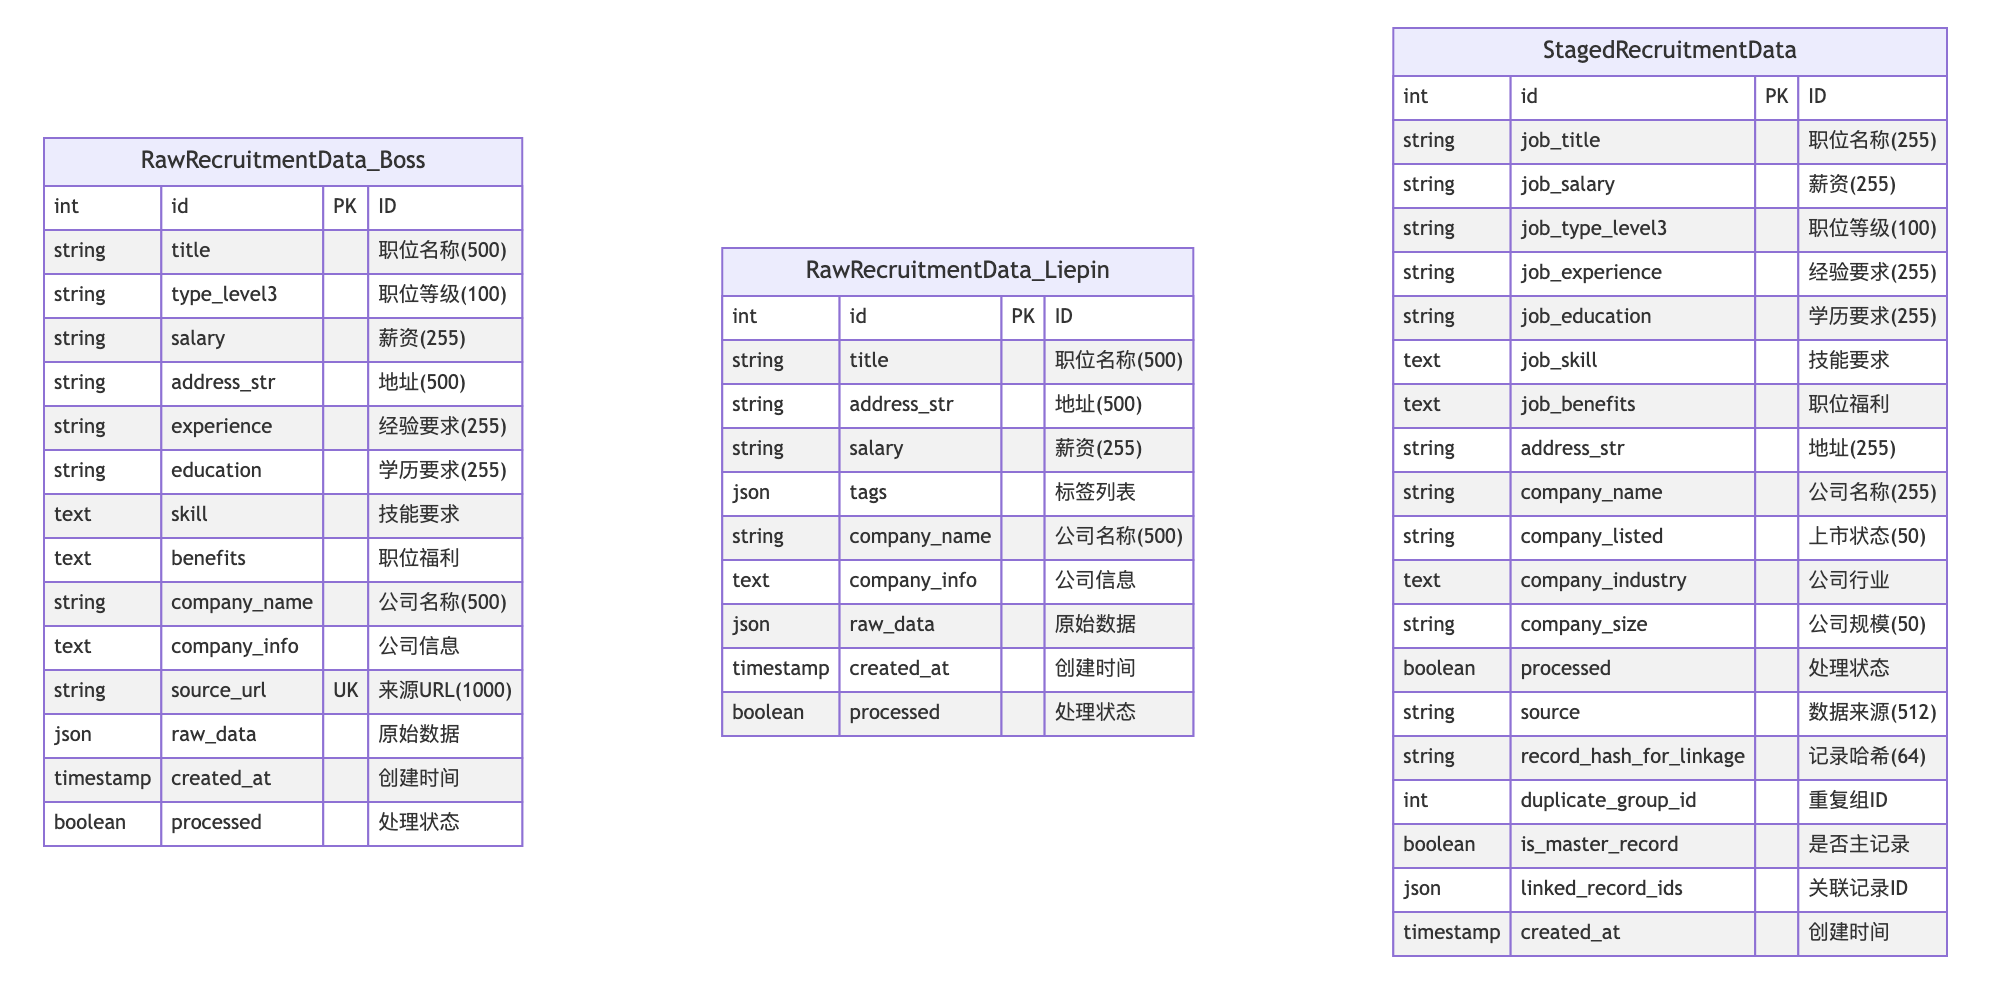
\includegraphics[width=0.8\textwidth]{figures/数据处理层ER图.png}
  \caption{数据处理层E-R图}
  \label{fig:processing_er}
\end{figure}

\paragraph{原始数据表设计}
如表\ref{tab:raw_boss_data_fields}和表\ref{tab:raw_liepin_data_fields}所示,系统包含两个原始数据表,分别对应不同的数据来源:

\begin{table}[htbp]
  \centering
  \caption{BOSS直聘原始数据表字段设计}
  \label{tab:raw_boss_data_fields}
  \begin{tabular}{@{}lll@{}}
    \toprule
    \textbf{字段类型} & \textbf{字段名} & \textbf{说明} \\
    \midrule
    \multirow{3}{*}{基础信息}
    & id & 主键 \\
    & created\_at & 创建时间 \\
    & processed & 处理状态标记 \\
    \midrule
    \multirow{7}{*}{职位信息}
    & job\_title & 职位名称(500字符) \\
    & job\_level & 职位等级(100字符) \\
    & salary & 薪资(255字符) \\
    & experience & 经验要求(255字符) \\
    & education & 学历要求(255字符) \\
    & skills & 技能要求(文本) \\
    & benefits & 职位福利(文本) \\
    \midrule
    \multirow{2}{*}{公司信息}
    & company\_name & 公司名称(500字符) \\
    & company\_detail & 公司详细信息(文本) \\
    \midrule
    \multirow{3}{*}{其他信息}
    & address & 地址文本(500字符) \\
    & source\_url & 来源URL(1000字符,唯一约束) \\
    & raw\_data & 原始数据(JSON) \\
    \bottomrule
  \end{tabular}
\end{table}

\begin{table}[htbp]
  \centering
  \caption{猎聘网原始数据表字段设计}
  \label{tab:raw_liepin_data_fields}
  \begin{tabular}{@{}lll@{}}
    \toprule
    \textbf{字段类型} & \textbf{字段名} & \textbf{说明} \\
    \midrule
    \multirow{3}{*}{基础信息}
    & id & 主键 \\
    & created\_at & 创建时间 \\
    & processed & 处理状态标记 \\
    \midrule
    \multirow{2}{*}{职位信息}
    & job\_title & 职位名称(500字符) \\
    & salary & 薪资(255字符) \\
    \midrule
    \multirow{2}{*}{公司信息}
    & company\_name & 公司名称(500字符) \\
    & company\_detail & 公司详细信息(文本) \\
    \midrule
    \multirow{3}{*}{其他信息}
    & address & 地址文本(500字符) \\
    & tags & 标签列表(JSON) \\
    & raw\_data & 原始数据(JSON) \\
    \bottomrule
  \end{tabular}
\end{table}

\paragraph{暂存数据表设计}
如表\ref{tab:staged_recruitment_data_fields}所示,暂存数据表(StagedRecruitmentData)作为数据清洗和转换的中间层:

\begin{table}[htbp]
  \centering
  \caption{暂存数据表字段设计}
  \label{tab:staged_recruitment_data_fields}
  \begin{tabular}{@{}lll@{}} 
    \toprule
    \textbf{字段类型} & \textbf{字段名} & \textbf{说明} \\ 
    \midrule
    \multirow{7}{*}{职位相关字段} 
    & job\_title & 职位名称(255字符) \\
    & job\_salary & 薪资描述(255字符) \\
    & job\_type\_level3 & 职位等级(100字符) \\
    & job\_experience & 经验要求(255字符) \\
    & job\_education & 学历要求(255字符) \\
    & job\_skill & 技能要求(文本) \\
    & job\_benefits & 职位福利(文本) \\
    \midrule
    \multirow{4}{*}{公司相关字段}
    & company\_name & 公司名称(255字符) \\
    & company\_listed & 上市状态(50字符) \\
    & company\_industry & 公司行业(文本) \\
    & company\_size & 公司规模(50字符) \\
    \midrule
    \multirow{6}{*}{数据处理相关字段}
    & processed & 处理状态标记(布尔值) \\
    & source & 数据来源标识(512字符) \\
    & record\_hash\_for\_linkage & 记录哈希值(64字符),用于快速判断重复 \\
    & duplicate\_group\_id & 重复记录组ID \\
    & is\_master\_record & 主记录标记(布尔值) \\
    & linked\_record\_ids & 关联记录ID列表(JSON) \\
    \bottomrule
  \end{tabular}
\end{table}

\subsection{关系模式设计}

\subsubsection{规范化数据层关系模式}

用户关系模式、公司关系模式、职位关系模式、地址关系模式、公司-地址关系模式、职位-地址关系模式的定义分别如代码\ref{lst:user_schema}-\ref{lst:job_address_schema}所示。


  \begin{listing}[htbp]
    \begin{minted}{sql}
User(
    id: Integer (PK),
    username: String(50) NOT NULL UNIQUE,
    password: String(50) NOT NULL,
    role: Enum('user', 'admin') NOT NULL DEFAULT 'user',
    created_at: DateTime NOT NULL
)
    \end{minted}
    \caption{用户表结构}\label{lst:user_schema}
  \end{listing}

  \begin{listing}[htbp]
    \begin{minted}{sql}
Company(
    id: Integer (PK),
    name: String(500) NOT NULL UNIQUE,
    industry: String(200),
    size: String(50),
    created_at: DateTime NOT NULL,
    updated_at: DateTime NOT NULL
)
    \end{minted}
    \caption{公司表结构}\label{lst:company_schema}
  \end{listing}

  \begin{listing}[htbp]
    \begin{minted}{sql}
Job(
    id: Integer (PK),
    title: String(500) NOT NULL,
    type_level3: String(100),
    salary: String(100),
    experience: String(100),
    education: String(100),
    skill: Text,
    benefits: Text,
    source: String(512),
    company_id: Integer (FK -> Company.id),
    raw_job_id: Integer (FK -> StagedRecruitmentData.id),
    created_at: DateTime NOT NULL,
    updated_at: DateTime NOT NULL
)
    \end{minted}
    \caption{职位表结构}\label{lst:job_schema}
  \end{listing}

  \begin{listing}[htbp]
    \begin{minted}{sql}
Address(
    id: Integer (PK),
    address_str: String(200) NOT NULL,
    latitude: Float,
    longitude: Float,
    created_at: DateTime NOT NULL,
    updated_at: DateTime NOT NULL
)
    \end{minted}
    \caption{地址表结构}\label{lst:address_schema}
  \end{listing}

  \begin{listing}[htbp]
    \begin{minted}{sql}
company_address(
    company_id: Integer (PK, FK -> Company.id),
    address_id: Integer (PK, FK -> Address.id),
    created_at: DateTime NOT NULL
)
    \end{minted}
    \caption{公司-地址关系表结构}\label{lst:company_address_schema}
  \end{listing}

  \begin{listing}[htbp]
    \begin{minted}{sql}
job_address(
    job_id: Integer (PK, FK -> Job.id),
    address_id: Integer (PK, FK -> Address.id),
    created_at: DateTime NOT NULL
)
    \end{minted}
    \caption{职位-地址关系表结构}\label{lst:job_address_schema}
  \end{listing}

\subsubsection{数据处理层关系模式}

BOSS直聘原始数据关系模式、猎聘网原始数据关系模式和暂存数据关系模式的定义分别如代码\ref{lst:raw_boss_schema}-\ref{lst:staged_data_schema}所示。

  \begin{listing}[htbp]
    \begin{minted}{sql}
RawRecruitmentData_Boss(
    id: Integer (PK),
    title: String(500),
    type_level3: String(100),
    salary: String(255),
    address_str: String(500),
    experience: String(255),
    education: String(255),
    skill: Text,
    benefits: Text,
    company_name: String(500),
    company_info: Text,
    source_url: String(1000) UNIQUE,
    raw_data: JSON,
    created_at: DateTime NOT NULL,
    processed: Boolean DEFAULT FALSE
)
    \end{minted}
    \caption{BOSS直聘原始数据表结构}\label{lst:raw_boss_schema}
  \end{listing}

  \begin{listing}[htbp]
    \begin{minted}{sql}
RawRecruitmentData_Liepin(
    id: Integer (PK),
    title: String(500),
    address_str: String(500),
    salary: String(255),
    tags: JSON,
    company_name: String(500),
    company_info: Text,
    raw_data: JSON,
    created_at: DateTime NOT NULL,
    processed: Boolean DEFAULT FALSE
)
    \end{minted}
    \caption{猎聘网原始数据表结构}\label{lst:raw_liepin_schema}
  \end{listing}

  \begin{listing}[htbp]
    \begin{minted}{sql}
StagedRecruitmentData(
    id: Integer (PK),
    job_title: String(255),
    job_salary: String(255),
    job_type_level3: String(100),
    job_experience: String(255),
    job_education: String(255),
    job_skill: Text,
    job_benefits: Text,
    address_str: String(255),
    company_name: String(255),
    company_listed: String(50),
    company_industry: Text,
    company_size: String(50),
    source: String(512),
    record_hash_for_linkage: String(64),
    duplicate_group_id: Integer,
    is_master_record: Boolean DEFAULT FALSE,
    linked_record_ids: JSON,
    processed: Boolean DEFAULT FALSE,
    created_at: DateTime NOT NULL
)
    \end{minted}
    \caption{暂存数据表结构}\label{lst:staged_data_schema}
  \end{listing}

\subsection{完整性约束设计}

\subsubsection{实体完整性约束}

\begin{enumerate}
  \item 主键约束
  \begin{itemize}
    \item 所有表都使用自增整数id作为主键,确保每条记录的唯一标识
    \item 关系表使用联合主键:
    \begin{itemize}
      \item company\_address表使用(company\_id, address\_id)作为联合主键
      \item job\_address表使用(job\_id, address\_id)作为联合主键
      \item 联合主键可以防止重复关联关系的产生
    \end{itemize}
  \end{itemize}

  \item 唯一性约束
  \begin{itemize}
    \item User表的username字段设置唯一约束,确保用户名不重复
    \item Company表的name字段设置唯一约束,避免重复录入公司信息
    \item RawRecruitmentData\_Boss表的source\_url字段设置唯一约束,防止重复爬取
    \item StagedRecruitmentData表的record\_hash\_for\_linkage字段设置唯一约束,用于数据去重
  \end{itemize}
\end{enumerate}

\subsubsection{参照完整性约束}

\begin{enumerate}
  \item 外键约束设计
  
  数据库中的外键约束主要体现在三个方面:Job表与Company表及StagedRecruitmentData表的关联、company\_address关系表的双向关联、以及job\_address关系表的双向关联。如\cref{lst:foreign_keys}所示,这些外键约束确保了数据的引用完整性。其中,Job表通过company\_id关联到Company表,通过raw\_job\_id关联到StagedRecruitmentData表;company\_address表通过company\_id和address\_id分别关联到Company表和Address表;job\_address表则通过job\_id和address\_id分别关联到Job表和Address表。

  \begin{listing}[htbp]
    \begin{minted}{sql}
-- Job表的外键约束
ALTER TABLE Job ADD CONSTRAINT fk_job_company
    FOREIGN KEY (company_id) REFERENCES Company(id);
ALTER TABLE Job ADD CONSTRAINT fk_job_staged
    FOREIGN KEY (raw_job_id) REFERENCES StagedRecruitmentData(id);

-- company_address表的外键约束
ALTER TABLE company_address ADD CONSTRAINT fk_company_address_company
    FOREIGN KEY (company_id) REFERENCES Company(id);
ALTER TABLE company_address ADD CONSTRAINT fk_company_address_address
    FOREIGN KEY (address_id) REFERENCES Address(id);

-- job_address表的外键约束
ALTER TABLE job_address ADD CONSTRAINT fk_job_address_job
    FOREIGN KEY (job_id) REFERENCES Job(id);
ALTER TABLE job_address ADD CONSTRAINT fk_job_address_address
    FOREIGN KEY (address_id) REFERENCES Address(id);
    \end{minted}
    \caption{外键约束定义}\label{lst:foreign_keys}
  \end{listing}

  \item 级联操作策略
  
  为了确保数据的安全性和一致性,所有外键约束均采用RESTRICT策略。这意味着当尝试删除被其他表引用的记录时,数据库将阻止该操作(ON DELETE RESTRICT);同样,当尝试更新被引用的主键值时,也会被阻止(ON UPDATE RESTRICT)。系统不采用级联删除(CASCADE)机制,以防止因误操作导致大规模的数据丢失。所有需要进行的更新操作都通过应用层代码严格控制,以确保数据的一致性和完整性。
\end{enumerate}

\subsubsection{用户定义完整性约束}
对于用户定义完整性约束,主要包含三类约束:非空约束、默认值约束和检查约束。非空约束(如\cref{lst:not_null_constraints}所示)主要应用于User表的username、password和role字段,Company表的name字段,Job表的title和company\_id字段,以及Address表的address\_str字段,确保这些关键字段不能为空。默认值约束(如\cref{lst:default_constraints}所示)设置了User表role字段的默认值为'user',各数据处理表的processed字段默认值为FALSE,以及Company表和User表的时间戳字段默认值为当前时间。检查约束(如\cref{lst:check_constraints}所示)则对数据的有效性进行验证,包括User表role字段的取值范围限制,Address表经纬度的有效范围检查,以及Company表和Job表的时间戳先后顺序验证。

\begin{listing}[htbp]
    \begin{minted}{sql}
-- User表非空约束
ALTER TABLE User MODIFY username VARCHAR(50) NOT NULL;
ALTER TABLE User MODIFY password VARCHAR(50) NOT NULL;
ALTER TABLE User MODIFY role ENUM('user', 'admin') NOT NULL;

-- Company表非空约束
ALTER TABLE Company MODIFY name VARCHAR(500) NOT NULL;

-- Job表非空约束
ALTER TABLE Job MODIFY title VARCHAR(500) NOT NULL;
ALTER TABLE Job MODIFY company_id INTEGER NOT NULL;

-- Address表非空约束
ALTER TABLE Address MODIFY address_str VARCHAR(200) NOT NULL;
    \end{minted}
    \caption{非空约束定义}\label{lst:not_null_constraints}
  \end{listing}

\begin{listing}[htbp]
    \begin{minted}{sql}
-- 角色默认值
ALTER TABLE User ALTER role SET DEFAULT 'user';

-- 处理状态默认值
ALTER TABLE RawRecruitmentData_Boss ALTER processed SET DEFAULT FALSE;
ALTER TABLE RawRecruitmentData_Liepin ALTER processed SET DEFAULT FALSE;
ALTER TABLE StagedRecruitmentData ALTER processed SET DEFAULT FALSE;

-- 时间戳默认值
ALTER TABLE User ALTER created_at SET DEFAULT CURRENT_TIMESTAMP;
ALTER TABLE Company ALTER created_at SET DEFAULT CURRENT_TIMESTAMP;
ALTER TABLE Company ALTER updated_at SET DEFAULT CURRENT_TIMESTAMP;
    \end{minted}
    \caption{默认值约束定义}\label{lst:default_constraints}
  \end{listing}

\begin{listing}[htbp]
    \begin{minted}{sql}
-- 角色检查
ALTER TABLE User ADD CONSTRAINT check_user_role 
    CHECK (role IN ('user', 'admin'));

-- 经纬度范围检查
ALTER TABLE Address ADD CONSTRAINT check_latitude
    CHECK (latitude BETWEEN -90 AND 90);
ALTER TABLE Address ADD CONSTRAINT check_longitude
    CHECK (longitude BETWEEN -180 AND 180);

-- 时间戳有效性检查
ALTER TABLE Company ADD CONSTRAINT check_company_timestamps
    CHECK (updated_at >= created_at);
ALTER TABLE Job ADD CONSTRAINT check_job_timestamps
    CHECK (updated_at >= created_at);
    \end{minted}
    \caption{检查约束定义}\label{lst:check_constraints}
  \end{listing}

  \subsection{存储结构设计}

  \subsubsection{数据库选型}
  \begin{itemize}
    \item 选用PostgreSQL 数据库系统
    \begin{itemize}
      \item 支持JSON类型,用于存储爬虫原始数据(raw\_data字段)和地址聚合(addresses字段)
      \item 支持物化视图,用于预计算recruitment\_mv,提升查询性能
      \item 支持gin\_trgm\_ops操作符,用于地址和公司名称的模糊匹配
      \item 支持异步SQLAlchemy,实现高并发数据处理
      \item 内置的MVCC机制,保证数据一致性
    \end{itemize}
    \item 数据库配置
    \begin{itemize}
      \item 连接池:使用SQLAlchemy的异步会话管理
      \item 环境变量:通过.env文件配置数据库连接参数
      \item 时区处理:统一使用UTC时区存储时间戳
    \end{itemize}
  \end{itemize}
  
  \subsubsection{表空间组织}
  
  \begin{enumerate}
    \item 规范化数据层表空间
    \begin{itemize}
      \item 核心业务表:users, companies, jobs, addresses
      \begin{itemize}
        \item users表:用户认证和权限管理
        \item companies表:公司基本信息和元数据
        \item jobs表:职位详情和关联信息
        \item addresses表:地理位置和坐标数据
      \end{itemize}
      \item 关系映射表:company\_address, job\_address
      \begin{itemize}
        \item company\_address:多对多关系,支持一个公司多个地址
        \item job\_address:多对多关系,支持一个职位多个工作地点
      \end{itemize}
      \item 物化视图:recruitment\_mv
      \begin{itemize}
        \item 预聚合职位、公司、地址信息
        \item 支持高性能的分页和统计查询
        \item 定时刷新保证数据一致性
      \end{itemize}
    \end{itemize}
  
    \item 数据处理层表空间
    \begin{itemize}
      \item 原始数据表:raw\_recruitment\_boss, raw\_recruitment\_liepin
      \begin{itemize}
        \item 存储爬虫直接获取的JSON数据
        \item 使用processed标志位跟踪处理状态
        \item 保留source\_url确保数据不重复爬取
      \end{itemize}
      \item 暂存数据表:staged\_recruitment\_data
      \begin{itemize}
        \item 统一格式的中间表,存储清洗后的数据
        \item 支持跨来源的记录去重和链接
        \item 使用record\_hash\_for\_linkage优化相似度计算
        \item 通过duplicate\_group\_id和is\_master\_record管理重复记录
      \end{itemize}
    \end{itemize}
  \end{enumerate}
  
  \subsubsection{字段类型选择}
  
  在设计数据库字段类型时,我们需要根据数据的特征和使用场景选择合适的类型,以平衡存储空间、查询性能和数据完整性。表\ref{tab:field_types}展示了本系统中使用的主要字段类型及其应用场景。
  
  对于标识符字段,我们选择Integer类型作为主键和外键,这不仅节省存储空间,还能通过自增特性避免键值碎片,提高数据库性能。在PostgreSQL中,Integer类型的自增主键会被自动创建聚集索引,有利于提升查询效率。
  
  文本类型的选择上,我们根据内容长度的不同采用了String和Text两种类型。对于长度固定或者有明确上限的字段(如用户名、角色等),使用String类型并指定合适的长度限制;对于可能包含大量文本的字段(如职位描述、公司简介等),则使用Text类型以节省存储空间。特别地,对于枚举类型的字段(如用户角色),我们使用PostgreSQL的Enum类型来确保数据的有效性。
  
  为了处理复杂的非结构化数据,我们充分利用了PostgreSQL对JSON类型的支持。原始爬虫数据和需要灵活扩展的字段(如标签数据、地址列表等)都使用JSON类型存储,这不仅提供了灵活的数据结构,还能通过PostgreSQL的JSON操作符实现高效的查询。
  
  表\ref{tab:field_lengths}详细列出了各个表中字符串类型字段的长度限制。这些限制是基于实际数据分析得出的,既要确保能够容纳正常数据,又要避免过度分配空间。例如,公司名称和职位名称的长度限制设置为500,这是考虑到中文公司名称可能较长,而且可能包含附加信息;而用户名等字段则限制在50个字符以内,这对于标识用途来说已经足够。
  
  对于时间相关的字段,我们统一使用带时区的DateTime类型,并通过SQLAlchemy的配置确保所有时间戳都以UTC时区存储。这样不仅能够准确记录时间信息,还能避免因时区差异导致的问题。created\_at和updated\_at这两个时间戳字段在大多数表中都会使用,用于追踪记录的创建和修改时间。
  
  \begin{table}[!htbp]
    \caption{数据库字段类型设计}
    \label{tab:field_types}
    \centering
    \begin{tabular}{@{}llll@{}} \toprule
      \textbf{类型分类} & \textbf{具体类型} & \textbf{应用场景} & \textbf{优点} \\ \midrule
      标识符字段 & Integer & 主键、外键 & 存储空间小,连接效率高 \\
                &         & id字段自增 & 避免键值碎片 \\ \midrule
      文本字段   & String(50) & 用户名、角色枚举 & 定长存储,性能好 \\
                & String(500) & 公司名称、职位名称 & 适应较长文本 \\
                & Text & 技能描述、职位福利 & 变长存储,节省空间 \\
                & Enum & 用户角色(UserRole) & 约束取值范围 \\ \midrule
      JSON字段   & JSON & 原始数据(raw\_data) & 灵活的数据结构 \\
                &      & 标签数据(tags) & 支持复杂查询 \\
                &      & 地址列表(addresses) & 支持索引优化 \\ \midrule
      时间戳字段 & DateTime & created\_at & 支持时区(UTC) \\
                &          & updated\_at & 自动更新时间戳 \\ \bottomrule
    \end{tabular}
  \end{table}
  
  \begin{table}[!htbp]
    \caption{字段长度限制设计}
    \label{tab:field_lengths}
    \centering
    \begin{tabular}{@{}lll@{}} \toprule
      \textbf{表名} & \textbf{字段名} & \textbf{长度限制} \\ \midrule
      users & username & String(50) \\
            & password & String(50) \\ \midrule
      companies & name & String(500) \\
               & industry & String(200) \\
               & size & String(50) \\ \midrule
      jobs & title & String(500) \\
           & type\_level3 & String(100) \\
           & salary & String(100) \\
           & experience & String(100) \\
           & education & String(100) \\ \midrule
      addresses & address\_str & String(200) \\ \bottomrule
    \end{tabular}
  \end{table}
  
  \subsection{索引设计}
  
  \subsubsection{基础索引}
  
  \begin{enumerate}
    \item 主键索引
    \begin{itemize}
      \item 所有表的id字段
      \item 类型:B-tree
      \item 特点:聚集索引
    \end{itemize}
  
    \item 外键索引(如代码\ref{lst:foreign_key_indexes}所示)
    \item 唯一索引(如代码\ref{lst:unique_indexes}所示)
  \end{enumerate}
  
  \begin{listing}[htbp]
    \begin{minted}{sql}
  -- Job表外键索引
  CREATE INDEX ix_jobs_company_id ON jobs(company_id);
  CREATE INDEX ix_jobs_raw_job_id ON jobs(raw_job_id);
    \end{minted}
    \caption{外键索引定义}\label{lst:foreign_key_indexes}
  \end{listing}
  
  \begin{listing}[htbp]
    \begin{minted}{sql}
  -- User表唯一索引
  CREATE UNIQUE INDEX ix_users_username ON users(username);
  
  -- Company表唯一索引
  CREATE UNIQUE INDEX ix_companies_name ON companies(name);
    \end{minted}
    \caption{唯一索引定义}\label{lst:unique_indexes}
  \end{listing}
  
  \subsubsection{复合索引}
  
  \begin{enumerate}
    \item 业务查询优化索引(如代码\ref{lst:composite_indexes}所示)
    \item 数据处理优化索引(如代码\ref{lst:processing_indexes}所示)
  \end{enumerate}
  
  \begin{listing}[htbp]
    \begin{minted}{sql}
  -- 公司查询优化
  CREATE INDEX ix_companies_industry_size ON companies(industry, size);
  CREATE INDEX ix_companies_name_industry ON companies(name, industry);
  
  -- 职位查询优化
  CREATE INDEX ix_jobs_title_type ON jobs(title, type_level3);
  CREATE INDEX ix_jobs_created_updated ON jobs(created_at, updated_at);
    \end{minted}
    \caption{复合索引定义}\label{lst:composite_indexes}
  \end{listing}
  
  \begin{listing}[htbp]
    \begin{minted}{sql}
  -- 原始数据处理状态索引
  CREATE INDEX ix_raw_recruitment_boss_processed_created 
  ON raw_recruitment_boss(processed, created_at);
  
  -- 暂存数据去重索引
  CREATE INDEX ix_staged_recruitment_data_record_hash_for_linkage 
  ON staged_recruitment_data(record_hash_for_linkage);
    \end{minted}
    \caption{数据处理索引定义}\label{lst:processing_indexes}
  \end{listing}
  
  \subsubsection{特殊索引}
  
  \begin{enumerate}
    \item GIN索引
    \begin{itemize}
      \item 用于全文搜索
      \item 支持模糊匹配
      \item 示例:
      \begin{minted}{sql}
  -- 地址文本搜索
  CREATE INDEX ix_addresses_address_str_trgm 
  ON addresses USING gin (address_str gin_trgm_ops);
      \end{minted}
    \end{itemize}
  
    \item B-tree索引
    \begin{itemize}
      \item 用于精确匹配和范围查询
      \item 支持多列复合索引
      \item 示例:
      \begin{minted}{sql}
  -- 公司查询优化
  CREATE INDEX ix_companies_industry_size 
  ON companies(industry, size);
      \end{minted}
    \end{itemize}
  
    \item 物化视图索引
    \begin{listing}[htbp]
      \begin{minted}{sql}
  -- 物化视图优化索引
  CREATE INDEX ix_recruitment_mv_title ON recruitment_mv(title);
  CREATE INDEX ix_recruitment_mv_company_name ON recruitment_mv(company_name);
  CREATE INDEX ix_recruitment_mv_created_at ON recruitment_mv(created_at);
      \end{minted}
      \caption{物化视图索引定义}\label{lst:materialized_view_indexes}
    \end{listing}
  \end{enumerate}
  
  \subsection{并发控制}
  
  \subsubsection{事务隔离级别}
  \begin{itemize}
    \item 读已提交(Read Committed)
    \begin{itemize}
      \item PostgreSQL默认隔离级别
      \item 防止脏读,允许不可重复读
      \item 支持MVCC,实现读写互不阻塞
    \end{itemize}
    \item 事务管理
    \begin{itemize}
      \item 使用SQLAlchemy的异步会话(AsyncSession)
      \item 支持嵌套事务(begin\_nested)
      \item 自动提交和回滚机制
    \end{itemize}
  \end{itemize}
  
  \subsubsection{并发访问优化}
  \begin{itemize}
    \item ETL并发处理
    \begin{itemize}
      \item 使用batch\_size控制批处理大小
      \item 通过processed标志位追踪处理状态
      \item 支持断点续传和错误重试
    \end{itemize}
    \item 记录链接优化
    \begin{itemize}
      \item 使用record\_hash快速判断重复
      \item 动态调整相似度阈值
      \item 分批处理避免长事务
    \end{itemize}
    \item 物化视图刷新
    \begin{itemize}
      \item 支持CONCURRENTLY并发刷新
      \item 通过调度器自动维护
      \item 避免阻塞在线查询
    \end{itemize}
  \end{itemize}

  
\subsubsection{后台服务层}
后台服务层负责系统的维护和监控工作,确保系统的稳定运行和数据的实时更新:

\begin{itemize}
    \item \textbf{物化视图更新}:
    \begin{itemize}
        \item 实现了基于时间触发的自动更新机制
        \item 支持手动触发的即时更新
        \item 提供了更新状态的监控接口
    \end{itemize}
    
    \item \textbf{任务调度器}:
    \begin{itemize}
        \item 基于APScheduler实现了灵活的任务调度系统
        \item 支持定时任务和周期性任务的管理
        \item 提供了任务执行状态的监控和告警
    \end{itemize}
    
    \item \textbf{系统监控}:
    \begin{itemize}
        \item 实现了全面的性能监控指标收集
        \item 提供了系统运行状态的实时监控
        \item 支持异常情况的自动告警
    \end{itemize}
\end{itemize}


\subsection{API实现}

系统的API层采用FastAPI框架实现,遵循RESTful架构设计原则,提供了一系列标准化的HTTP接口。API的实现主要分为以下几个模块:

\subsubsection{认证模块(/auth)}
认证模块负责用户的身份验证和授权管理:

\begin{itemize}
    \item \textbf{登录接口}:
    \begin{itemize}
        \item 路径:\texttt{/auth/login}
        \item 方法:POST
        \item 功能:验证用户身份并返回用户信息
        \item 实现:基于JWT的身份验证机制
    \end{itemize}
\end{itemize}

\subsubsection{任务管理模块(/tasks)}
任务管理模块负责系统中各种数据处理任务的管理和监控:

\begin{itemize}
    \item \textbf{任务状态查询}:
    \begin{itemize}
        \item 路径:\texttt{/tasks/status}
        \item 方法:GET
        \item 功能:获取指定任务的执行状态
    \end{itemize}
    
    \item \textbf{任务触发}:
    \begin{itemize}
        \item 路径:\texttt{/tasks/trigger/\{task\_name\}}
        \item 方法:POST
        \item 功能:手动触发指定的任务
    \end{itemize}
    
    \item \textbf{数据导入任务}:
    \begin{itemize}
        \item 路径:\texttt{/tasks/add-data/import-data-liepin-csv}
        \item 方法:POST
        \item 功能:导入猎聘网CSV数据
    \end{itemize}
    
    \item \textbf{数据处理任务}:
    \begin{itemize}
        \item 路径:\texttt{/tasks/add-data/process-data-boss}
        \item 方法:POST
        \item 功能:处理BOSS直聘原始数据
    \end{itemize}
    
    \item \textbf{地理编码任务}:
    \begin{itemize}
        \item 路径:\texttt{/tasks/add-data/encode-addresses}
        \item 方法:POST
        \item 功能:处理地址的地理编码
    \end{itemize}
\end{itemize}

\subsubsection{招聘信息模块(/recruitments)}
招聘信息模块提供职位相关的数据访问接口:

\begin{itemize}
    \item \textbf{职位列表查询}:
    \begin{itemize}
        \item 路径:\texttt{/recruitments/}
        \item 方法:GET
        \item 功能:支持分页、排序和过滤的职位信息查询
    \end{itemize}
    
    \item \textbf{职位详情查询}:
    \begin{itemize}
        \item 路径:\texttt{/recruitments/\{job\_id\}}
        \item 方法:GET
        \item 功能:获取指定职位的详细信息
    \end{itemize}
\end{itemize}

\subsubsection{公司信息模块(/companies)}
公司信息模块提供公司相关的数据访问接口:

\begin{itemize}
    \item \textbf{公司列表查询}:
    \begin{itemize}
        \item 路径:\texttt{/companies/}
        \item 方法:GET
        \item 功能:支持分页的公司信息查询
    \end{itemize}
    
    \item \textbf{公司详情查询}:
    \begin{itemize}
        \item 路径:\texttt{/companies/\{company\_id\}}
        \item 方法:GET
        \item 功能:获取指定公司的详细信息
    \end{itemize}
\end{itemize}

\subsubsection{可视化模块(/visualization)}
可视化模块提供各种数据分析和可视化接口,下面只给出部分接口的示例,完整接口请参考代码。如图\ref{fig:visualization_api}所示,可以看到后端fastapi的接口文档。

\begin{itemize}
    \item \textbf{薪资分布分析}:
    \begin{itemize}
        \item 路径:\texttt{/visualization/salary-distribution/\{salary\_type\}}
        \item 方法:GET
        \item 功能:获取不同类型的薪资分布数据
        \item 参数:支持平均薪资、最高薪资、最低薪资等类型
    \end{itemize}
    
    \item \textbf{职位分布分析}:
    \begin{itemize}
        \item 路径:\texttt{/visualization/job-title-distribution}
        \item 方法:GET
        \item 功能:获取职位名称的分布统计
    \end{itemize}
    
    \item \textbf{地理分布分析}:
    \begin{itemize}
        \item 路径:\texttt{/visualization/salary-heatmap}
        \item 方法:GET
        \item 功能:获取薪资的地理分布热力图
    \end{itemize}
    
    \item \textbf{教育经验分析}:
    \begin{itemize}
        \item 路径:\texttt{/visualization/education-experience-distribution}
        \item 方法:GET
        \item 功能:分析学历要求与经验要求的关系
    \end{itemize}
    
    \item \textbf{行业薪资分析}:
    \begin{itemize}
        \item 路径:\texttt{/visualization/industry-salary-stats}
        \item 方法:GET
        \item 功能:分析不同行业的薪资情况
        \item 参数:支持不同的排序方式和图表显示模式
    \end{itemize}
\end{itemize}

\begin{figure}[htbp]
    \centering
    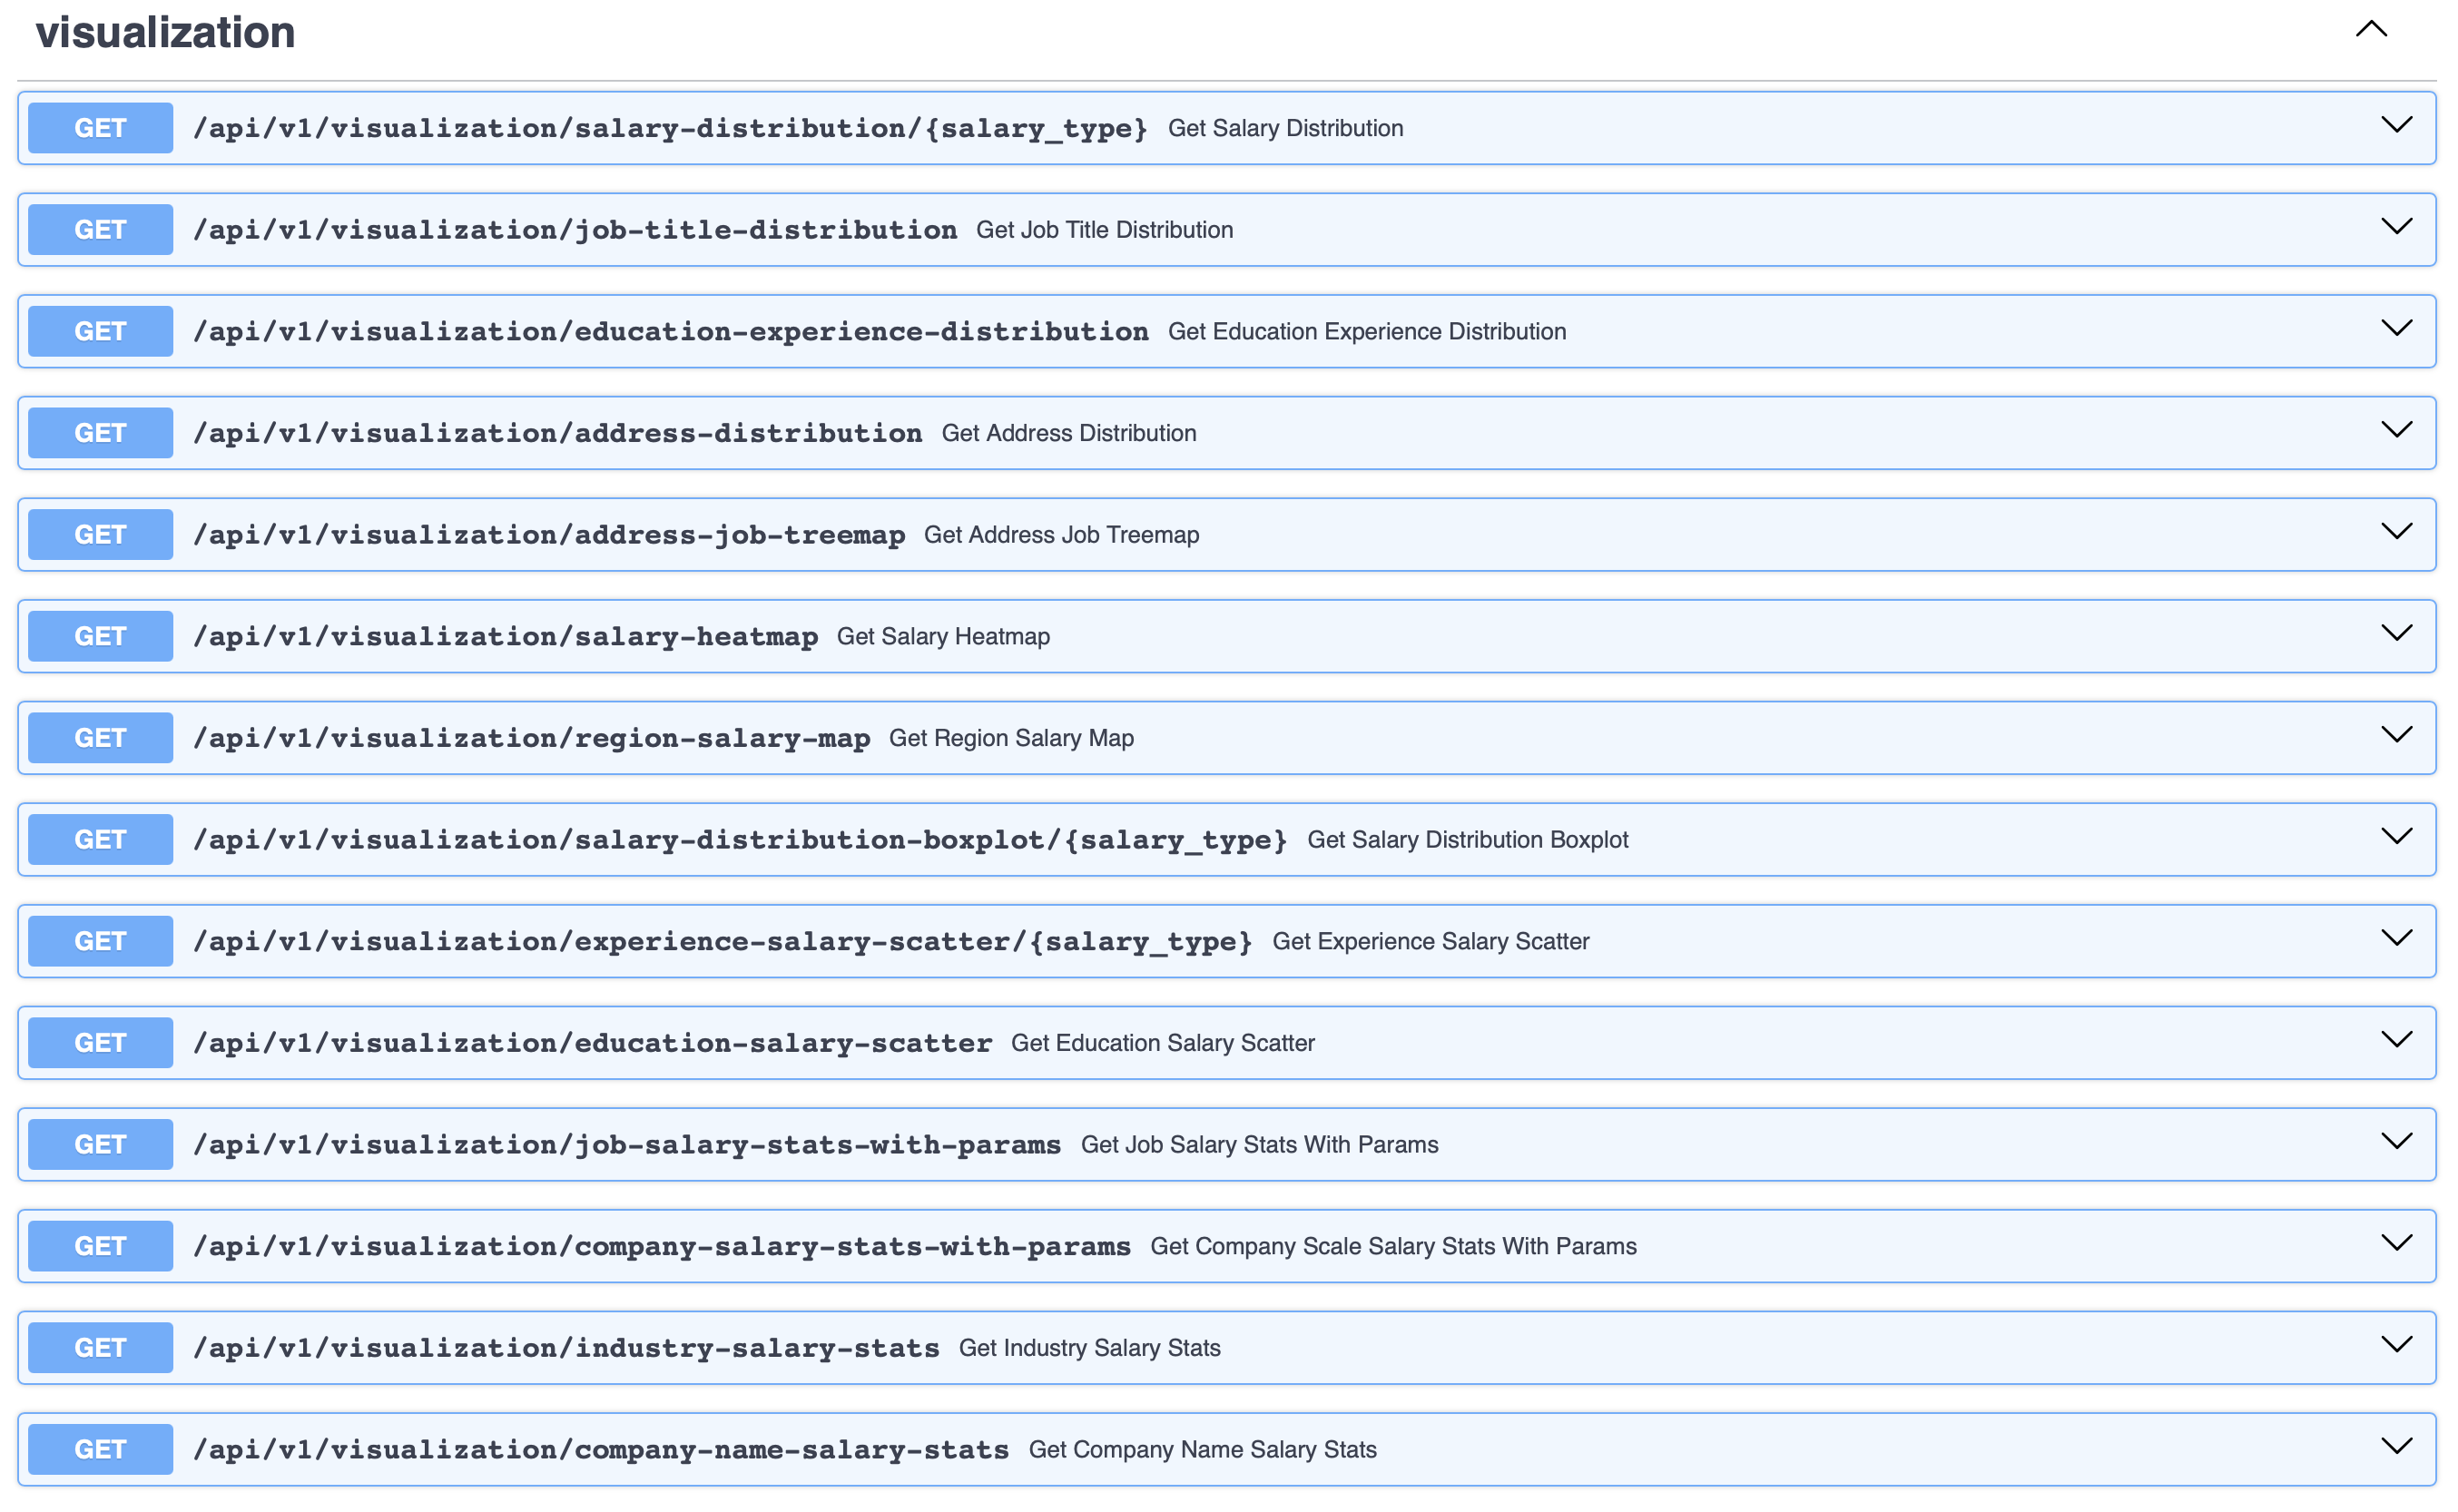
\includegraphics[width=0.9\textwidth]{figures/visualization_api.png}
    \caption{可视化模块API接口文档}
    \label{fig:visualization_api}
\end{figure}

\subsubsection{监控模块(/monitor)}
监控模块提供系统运行状态和数据质量的监控接口:

\begin{itemize}
    \item \textbf{数据质量监控}:
    \begin{itemize}
        \item 路径:\texttt{/monitor/data-quality}
        \item 方法:GET
        \item 功能:监控数据的完整性和质量
    \end{itemize}
    
    \item \textbf{数据一致性监控}:
    \begin{itemize}
        \item 路径:\texttt{/monitor/data-consistency}
        \item 方法:GET
        \item 功能:检查数据的一致性和完整性
    \end{itemize}
    
    \item \textbf{ETL进度监控}:
    \begin{itemize}
        \item 路径:\texttt{/monitor/etl-progress}
        \item 方法:GET
        \item 功能:监控ETL处理的进度
    \end{itemize}
    
    \item \textbf{系统性能监控}:
    \begin{itemize}
        \item 路径:\texttt{/monitor/system-performance}
        \item 方法:GET
        \item 功能:监控系统的性能指标
    \end{itemize}
\end{itemize}
\section{实现}
\subsection{数据采集}
职位信息作为招聘网站的核心要素,通常设有保护措施防止被大规模爬取。许多招聘网站
只允许登录用户查看职位信息。但同时,有些网站为了吸引流量,也会开放部分的岗位信息
给未登录用户浏览。在本项目中,我们挑选了两家允许未登录用户浏览职位的网站——\href{liepin.com}{猎聘网}和\href{zhipin.com}{BOSS直聘},用于采集所需要的职位信息。

\subsubsection{猎聘网数据的爬取}
图\ref{liepin}为猎聘的主页。点击位于导航栏的“职位”后,便可以跳转至图\ref{liepinJob}的职位展示页面。

\begin{figure}[!htbp]
    \centering
    
\includegraphics[width=\textwidth]{figures/liepin.png}
    \caption{猎聘主页}\label{liepin}
\end{figure}

\begin{figure}[!htbp]
    \centering
    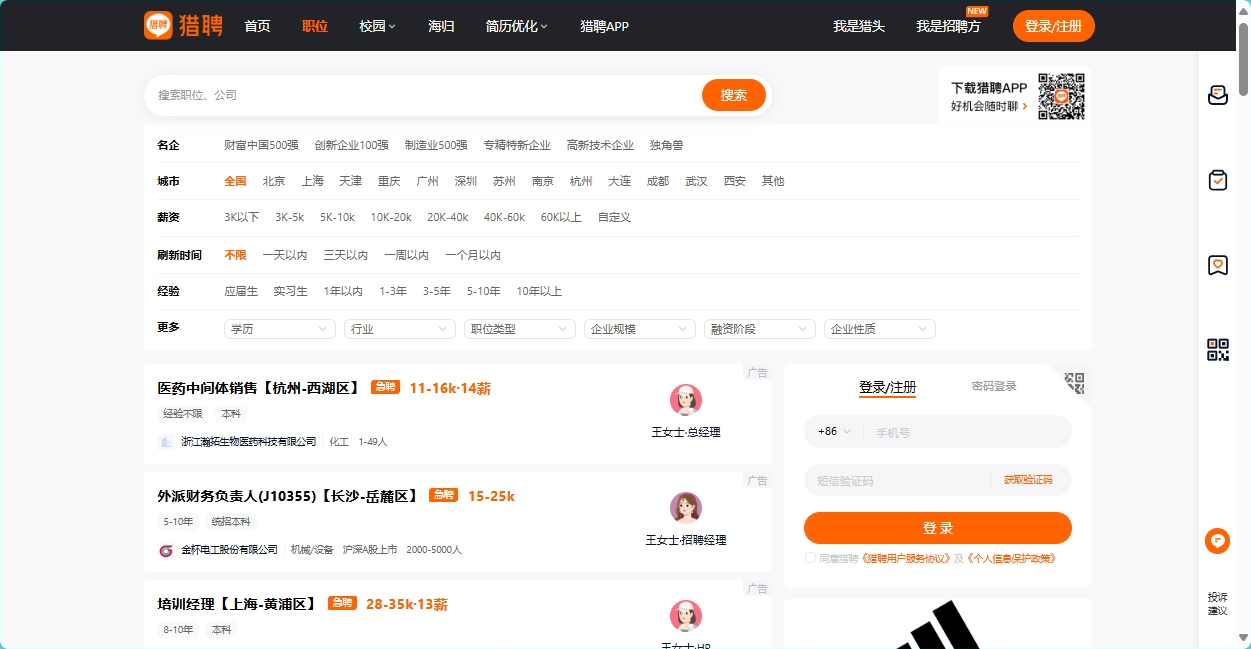
\includegraphics[width=\textwidth]{figures/liepinJob.png}
    \caption{猎聘职位页面}\label{liepinJob}
\end{figure}


如图\ref{response}所示,使用开发者工具查看网络情况,可以看到该页面上的职位信息是通过动态请求的方式获取到的。从图\ref{payload}
可以看出,响应的请求报文的载荷由两部分组成:1)职位的筛选条件;2)passThroughForm。其中,passThroughForm难以模拟,因此我们
放弃使用requests库进行爬取,而是使用selenium库进行后续的爬取。

\begin{figure}[!htbp]
    \centering
    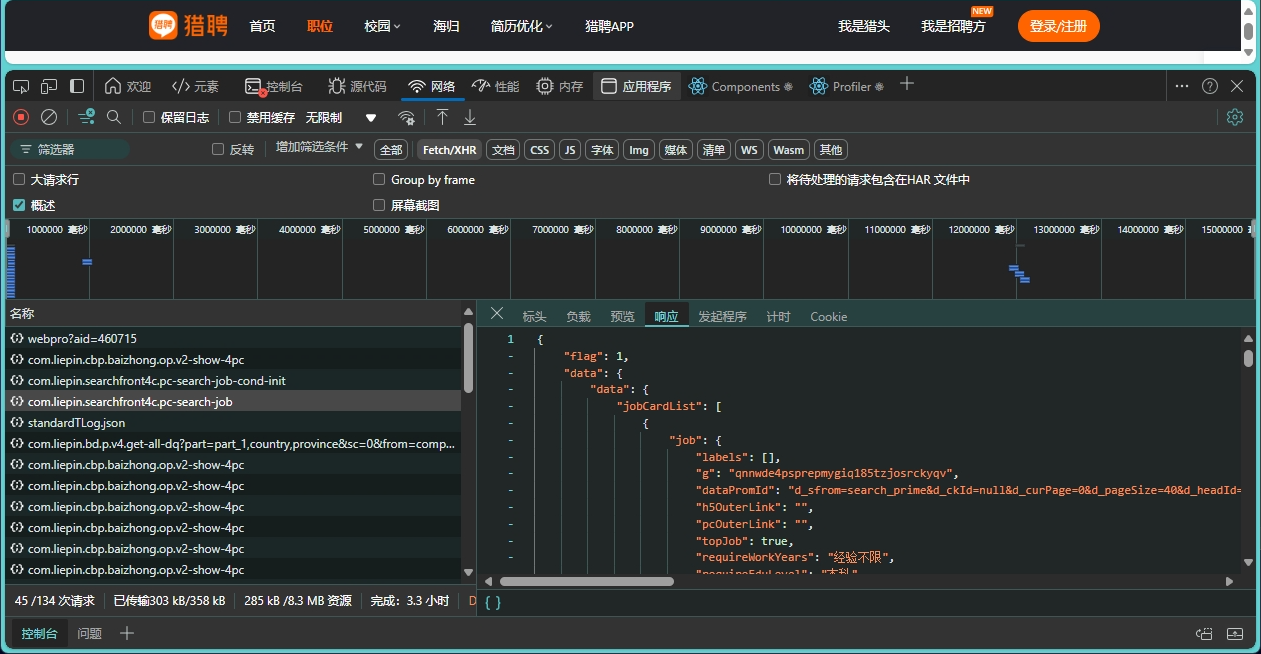
\includegraphics[width=\textwidth]{figures/response.png}
    \caption{含有职位数据的回复报文}\label{response}
\end{figure}

\begin{figure}[!htbp]
    \centering
    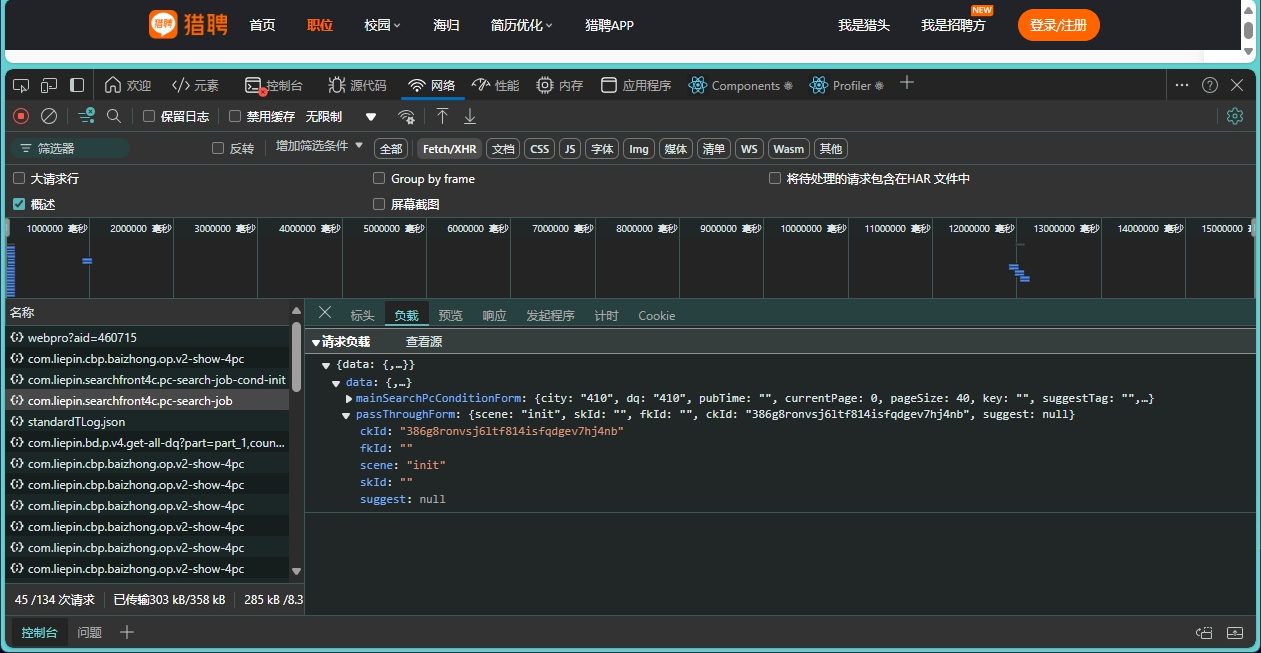
\includegraphics[width=\textwidth]{figures/payload.png}
    \caption{请求职位数据所需载荷}\label{payload}
\end{figure}

由于本项目的主题是“上海市信息类职位分析平台”。所以我们需要在城市筛选条件中选择“上海”,并且
在行业中选择“信息类”。同时,为了尽可能多地采集数据,我们会对“名企”、“薪资”、“经验”这三个条件的所有组合逐一进行爬取。
对于每个条件组合,我们都会创建一个selenium实例。

如图\ref{options}所示,我们可以通过 \texttt{filter-options-row-section}来定位到筛选条件按钮所在区域;根据 \texttt{row-title}中的内容来确定是什么筛选条件;
根据 \texttt{data-name}来定位具体的条件对应元素。



\begin{figure}[!htbp]
    \centering
    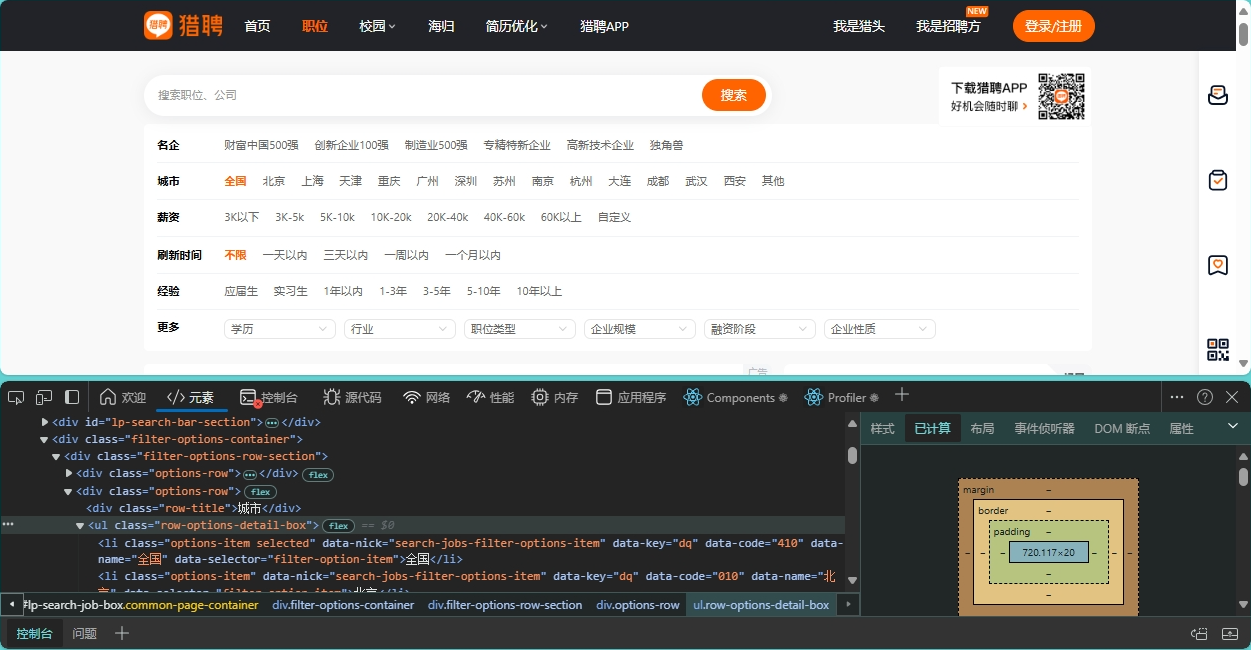
\includegraphics[width=\textwidth]{figures/options.png}
    \caption{职位筛选条件所在元素}\label{options}
\end{figure}

如图\ref{selector}所示,我们可以通过class名中带有 \texttt{select-industries-box}这一条件来定位到条件下拉框对应的元素,这可以通过查找XPATH来实现。

\begin{figure}[!htbp]
    \centering
    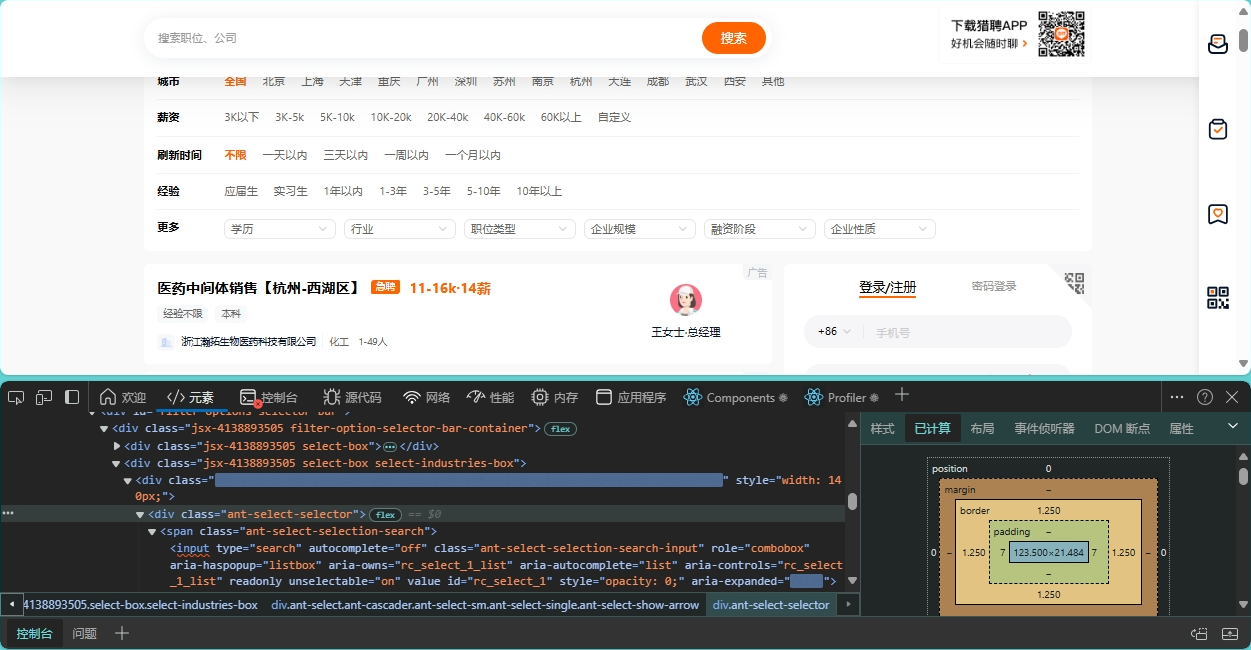
\includegraphics[width=\textwidth]{figures/selector.png}
    \caption{行业筛选条件所在元素}\label{selector}
\end{figure}

如图\ref{card}所示,我们可以通过class名为 \texttt{job-list-box}这一条件来获取各个职位卡片,然后遍历各个卡片,获取其中的职位信息。

\begin{figure}[!htbp]
    \centering
    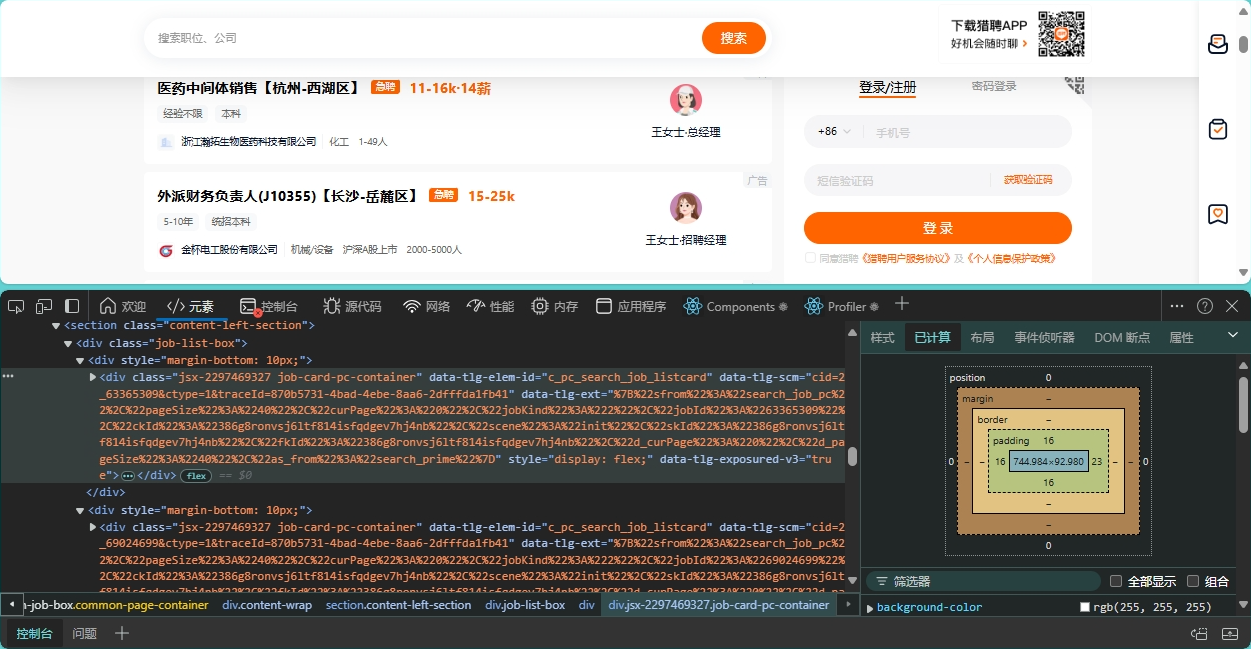
\includegraphics[width=\textwidth]{figures/card.png}
    \caption{职位信息所在元素}\label{card}
\end{figure}

如图\ref{nextpage}所示,我们可以通过 title对于 Next Page这一条件来定位到切换至下一页的按钮所在元素。可以通过该元素是否有效来判断是否已经是最后一页。

\begin{figure}[!htbp]
    \centering
    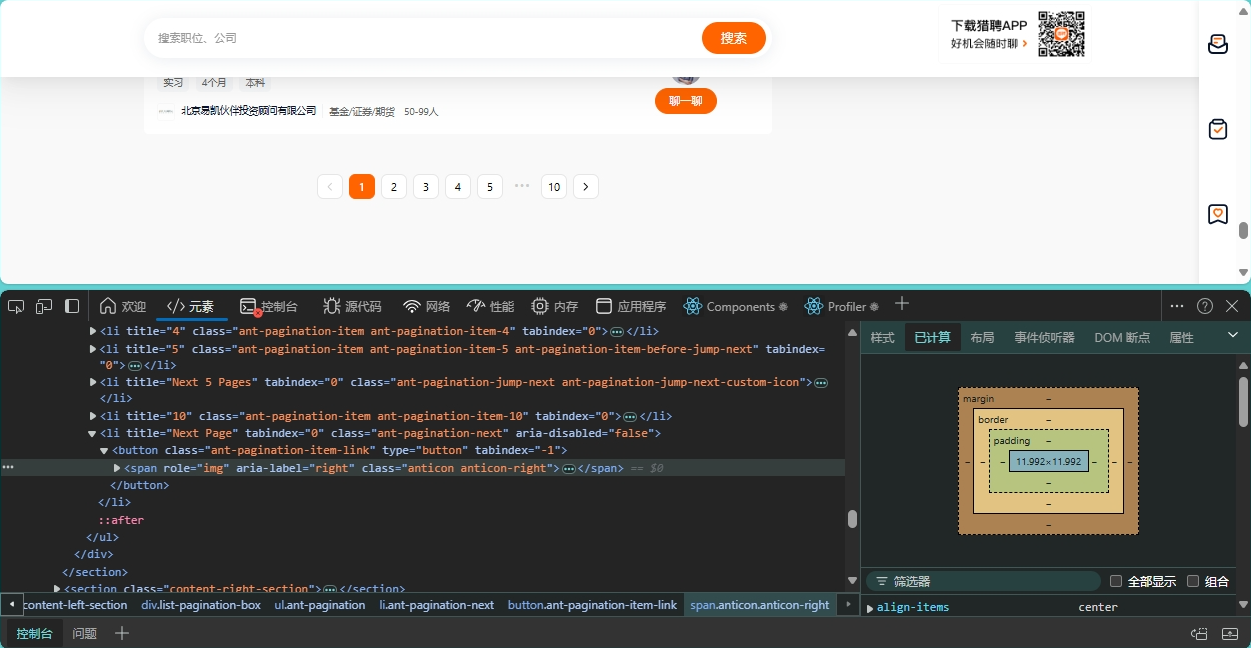
\includegraphics[width=\textwidth]{figures/nextpage.png}
    \caption{翻页按钮所在元素}\label{nextpage}
\end{figure}

在实际采集的过程中,经常会出现跳出如图\ref{login}所示的登录页的情况。为此,我们使用\href{www.qg.net}{青果网络}的隧道代理服务,每次创建一个selenium实例便更换一次IP地址。
同时,我们通过异常捕获机制允许对同一条件尝试10次,若失败次数到达10次,则记录到错误日志中,可以后续集中重新爬取。为了模拟人类行为,我们在每次操作之间增加了服从高斯分布的睡眠时间。

\begin{figure}[!htbp]
    \centering
    
\includegraphics[width=\textwidth]{figures/login.png}
    \caption{登录页}\label{login}
\end{figure}

在爬取的过程中,我们同步将获得的数据写入SQLite数据库。整个爬取过程用时约14个小时,共爬取近6000条数据。有15个条件组合爬取失败。

\subsubsection{BOSS直聘数据的爬取}

图\ref{BOSS}为BOSS直聘的首页。点击导航栏中的“搜索”,既可以跳转至图\ref{BOSSJob}中的职位搜索页,能够满足我们项目对于岗位的筛选需求。
该搜索网页的url为\texttt{https://www.zhipin.com/web/geek/job?query=},选择若干筛选条件后,可以看到url的变化仅为添加了相应的参数。例如,
在城市中选择“天津”,然后在区域中选择“西青区(全)”,再选择Java岗位类型,并限制为全职后,url变为\texttt{https://www.zhipin.com/web/geek/job?city=101030100\\\&position=100101\&jobType=1901\&areaBusiness=120111},
各参数的含义明确。因此我们首先尝试使用requests库,通过构造url的方式来进行爬取。经过尝试,我们发现必须要使用cookie才能成功申请到数据。
由于本项目所需采集的数据量较大,因此我们决定使用selenium进行爬取,避免了手动提取cookie的步骤。

与爬取猎聘网的过程不同,由于BOSS直聘的url容易模拟,我们可以直接通过selenium实例的get方法来直接设置所有的筛选条件,而无需通过通过模拟逐个点击筛选条件的方式。
这使得爬取BOSS直聘数据的速度较快,并且由于减少了与网页交互的次数,也更不容易被反爬虫技术所识别。

\begin{figure}[!htbp]
    \centering
    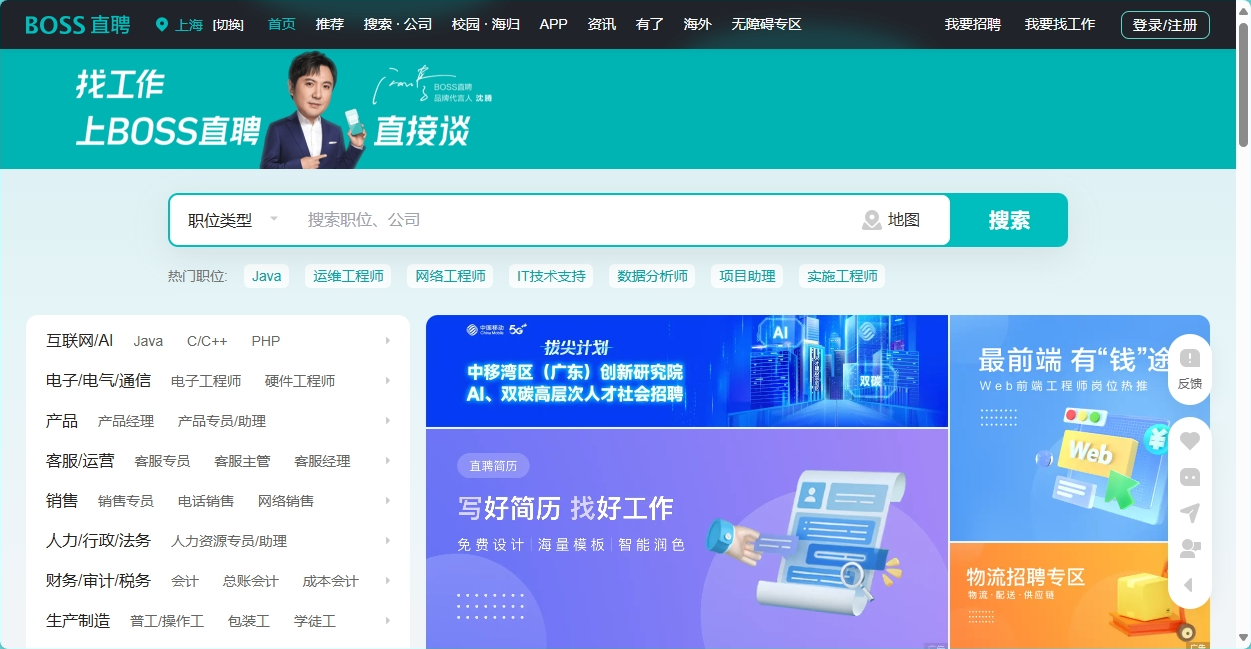
\includegraphics[width=\textwidth]{figures/BOSS}
    \caption{BOSS直聘主页}\label{BOSS}
\end{figure}

\begin{figure}[!htbp]
    \centering
    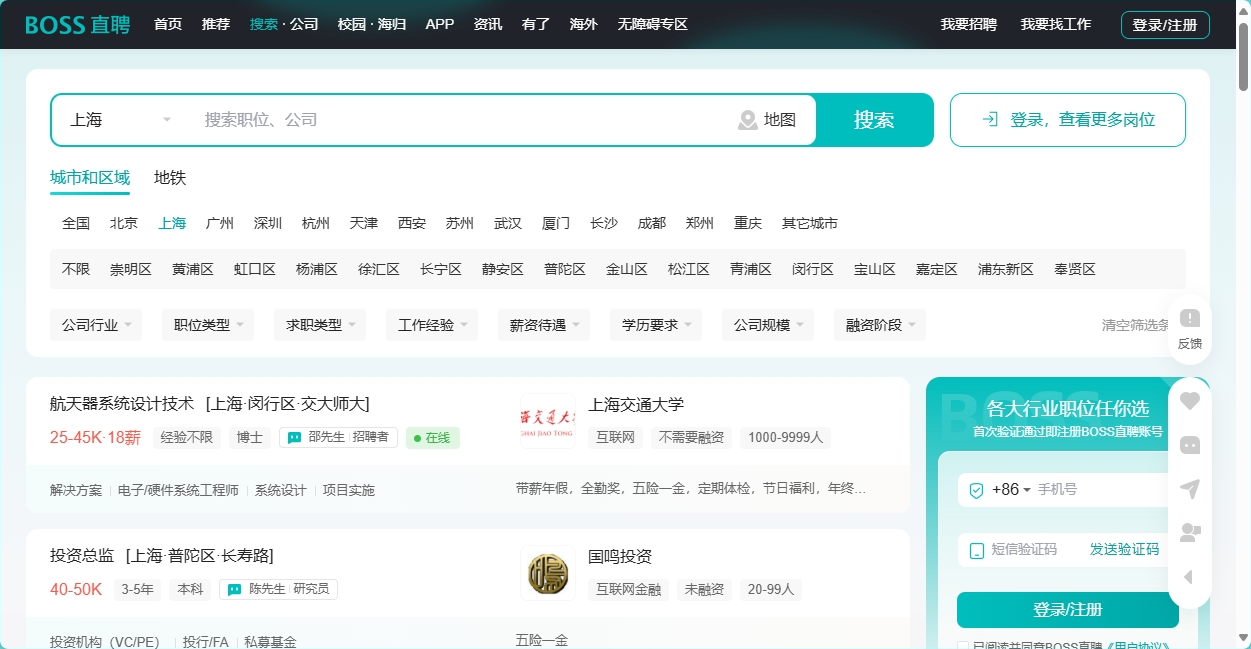
\includegraphics[width=\textwidth]{figures/BOSSJob.png}
    \caption{BOSS直聘搜索页面}\label{BOSSJob}
\end{figure}

如图\ref{wrapper}所示,我们可以通过class为\texttt{job-card-wrapper}这一条件来获取所有的工作卡片,从而进一步逐一从中提取岗位的具体信息。


\begin{figure}[!htbp]
    \centering
    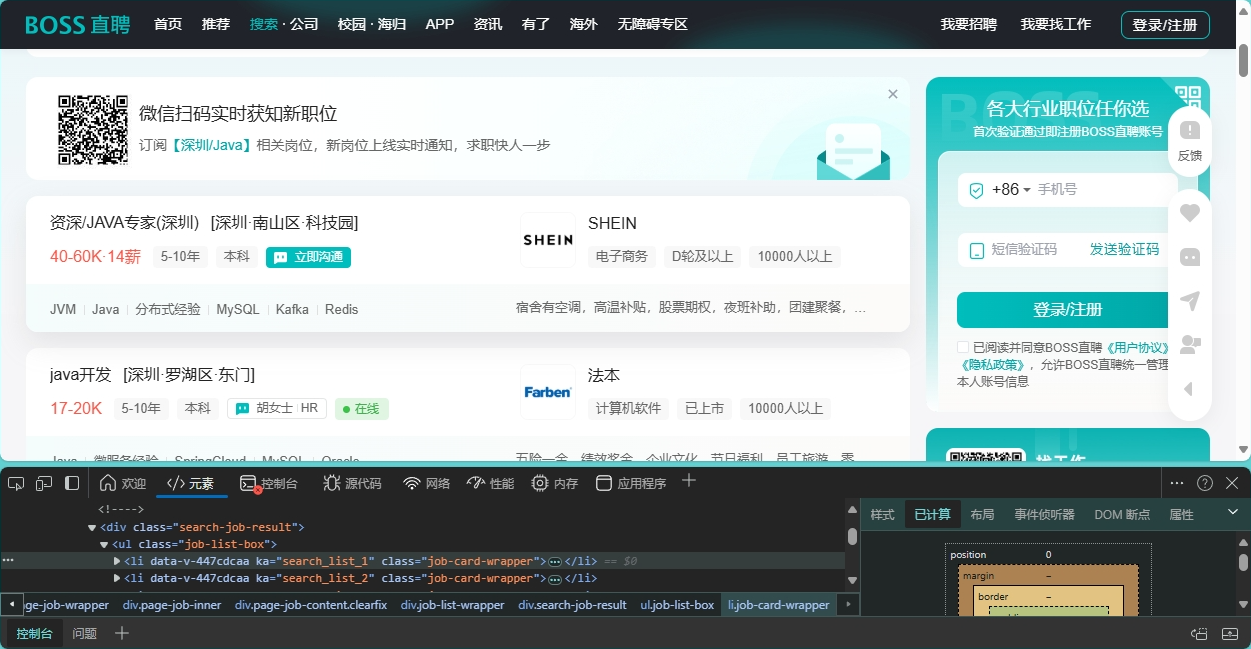
\includegraphics[width=\textwidth]{figures/wrapper.png}
    \caption{定位工作信息所在元素}\label{wrapper}
\end{figure}

如图\ref{next}所示,我们可以通过class为\texttt{ui-icon-arrow-right}这一条件来定位到翻页按钮所在元素。我们可以通过该元素是否启用来判断是否以及到达最后一页。
为了防止被识别为爬虫程序,我们采用\verb|ActionChains|类来模拟人类的行为。

\begin{figure}[!htbp]
    \centering
    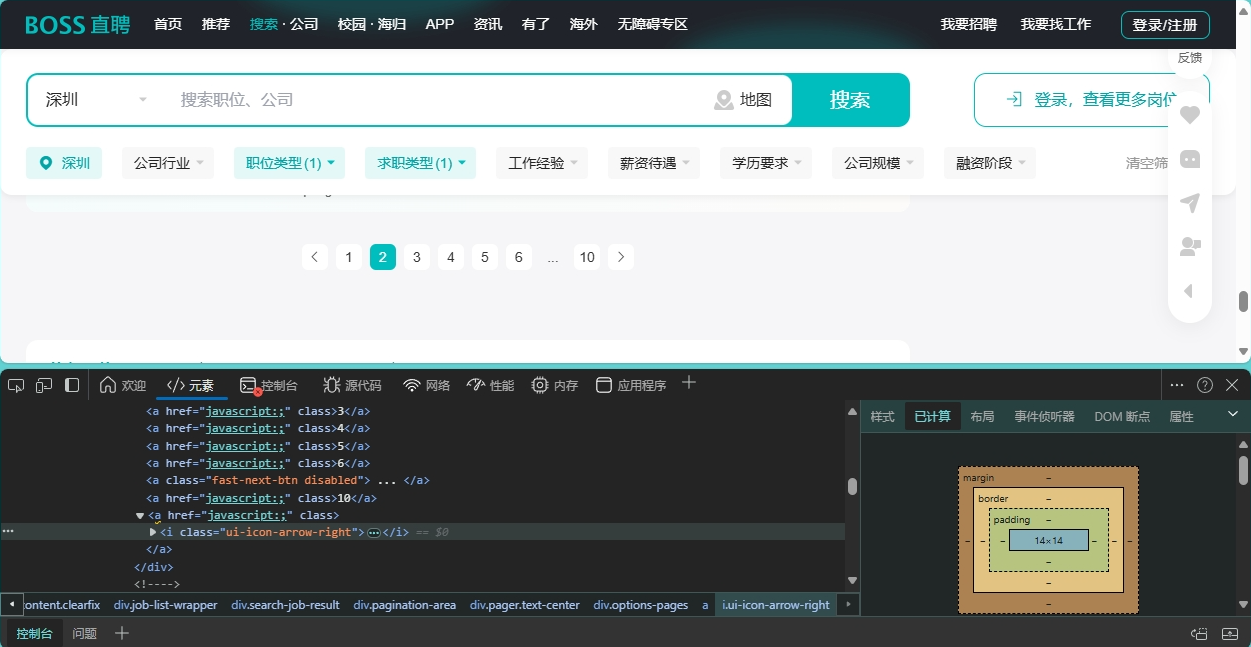
\includegraphics[width=\textwidth]{figures/next.png}
    \caption{翻页按钮所在元素}\label{next}
\end{figure}

\subsubsection{58招聘数据的爬取}

在数据采集的过程中,我们也尝试爬取58招聘网站的数据。图\ref{58}为58招聘网站的主页,点击导航栏中的社会招聘,将跳转至
图\ref{58job}中的岗位详情页面。

\begin{figure}[!htbp]
    \centering
    
\includegraphics[width=\textwidth]{figures/58.png}
    \caption{58招聘主页}\label{58}
\end{figure}

\begin{figure}[!htbp]
    \centering
    
\includegraphics[width=\textwidth]{figures/58job.png}
    \caption{58招聘岗位页面}\label{58job}
\end{figure}

如图\ref{58network}所示,通过开发者工具查看网络活动情况,我们发现该网页的岗位数据是通过动态请求的方式获取的,
相应的载荷如图\ref{58payload}所示。并且,通过开发者工具我们可以看到该请求的请求标头中不含有cookie。因此我们直接通过
requests库来获取。

\begin{figure}[!htbp]
    \centering
    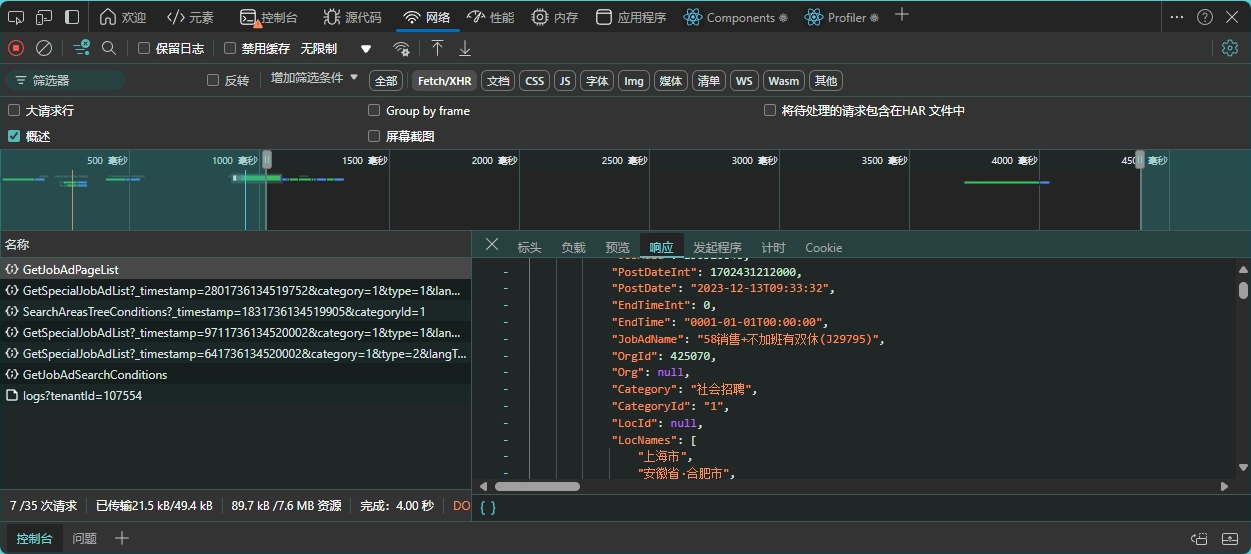
\includegraphics[width=\textwidth]{figures/58network.png}
    \caption{58招聘岗位页面网络请求情况}\label{58network}
\end{figure}

\begin{figure}[!htbp]
    \centering
    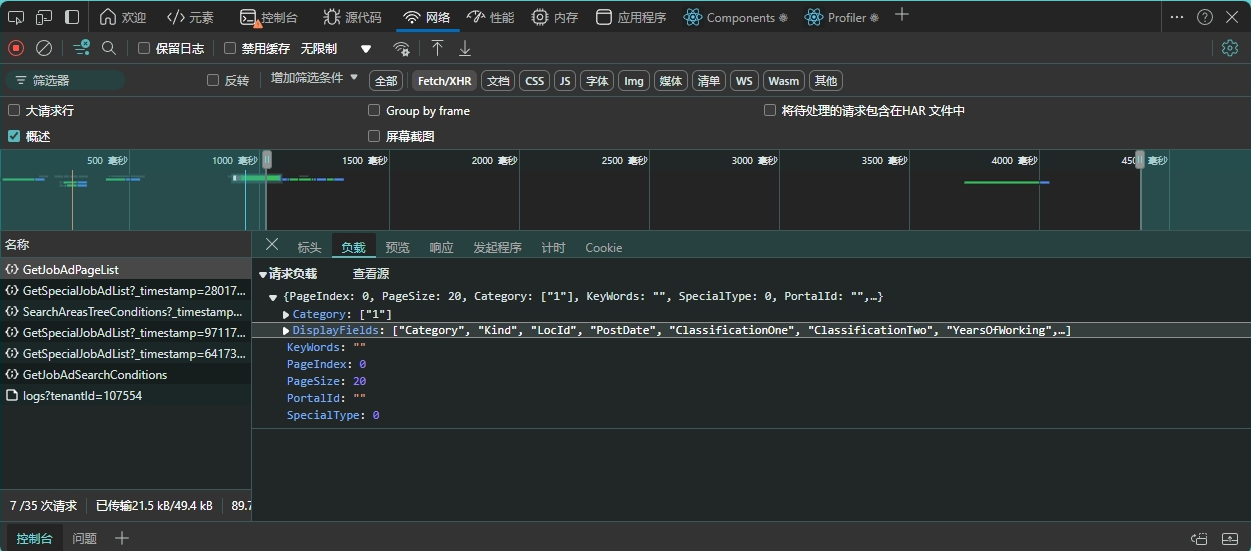
\includegraphics[width=\textwidth]{figures/58payload.png}
    \caption{58招聘岗位信息请求所需负载}\label{58payload}
\end{figure}

一条典型的工作岗位数如图\ref{data}所示。可以看到,该网站所返回的字段有大量的缺失值,例如\texttt{Salary},\texttt{Degree},\texttt{YearOfWorking}等。
这些信息都被集中在\texttt{Duty},\texttt{Require}字段中。
同时,我们发现58招聘网站上发布的岗位信息与先前爬取的猎聘网和BOSS直聘网的岗位数据有较大不同。例如58招聘网中的岗位信息中不包含公司名称,
薪资大多是“面谈”。上述这些特点都给后续的数据集成阶段带来较多不便,因此,在数据集成阶段,我们只采用猎聘网和BOSS直聘网的数据。

\begin{figure}[!htbp]
    \centering
    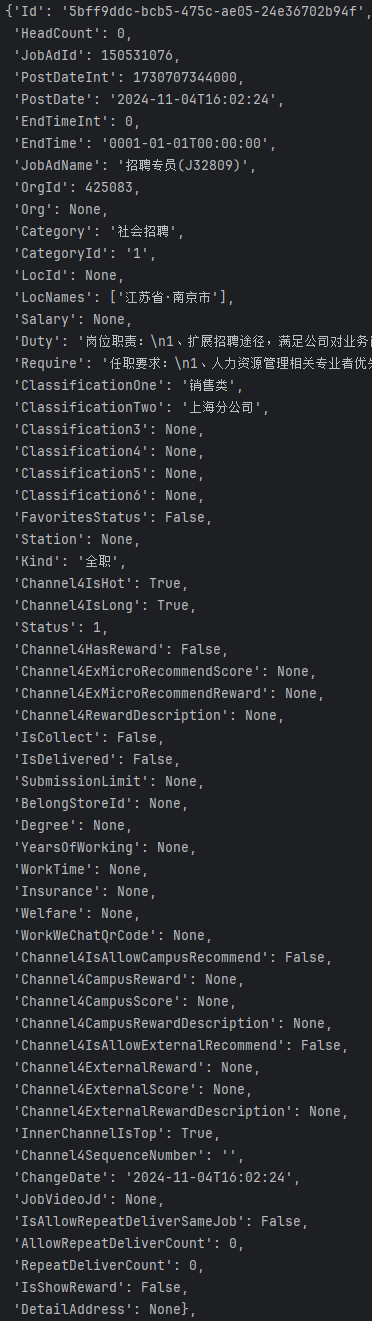
\includegraphics[height=0.8\textheight]{figures/data.png}
    \caption{58招聘岗位数据示例}\label{data}
\end{figure}


\subsection{数据集成}
本系统实现了一个完整的ETL(Extract-Transform-Load)数据集成流程,将来自不同招聘网站的职位数据进行整合、清洗和标准化,最终加载到规范化的数据库中。整个过程包括数据抽取(Extract)、数据转换(Transform)和数据加载(Load)三个主要阶段。如图\ref{fig:ETL}所示。

\begin{figure}[htbp]
    \centering
    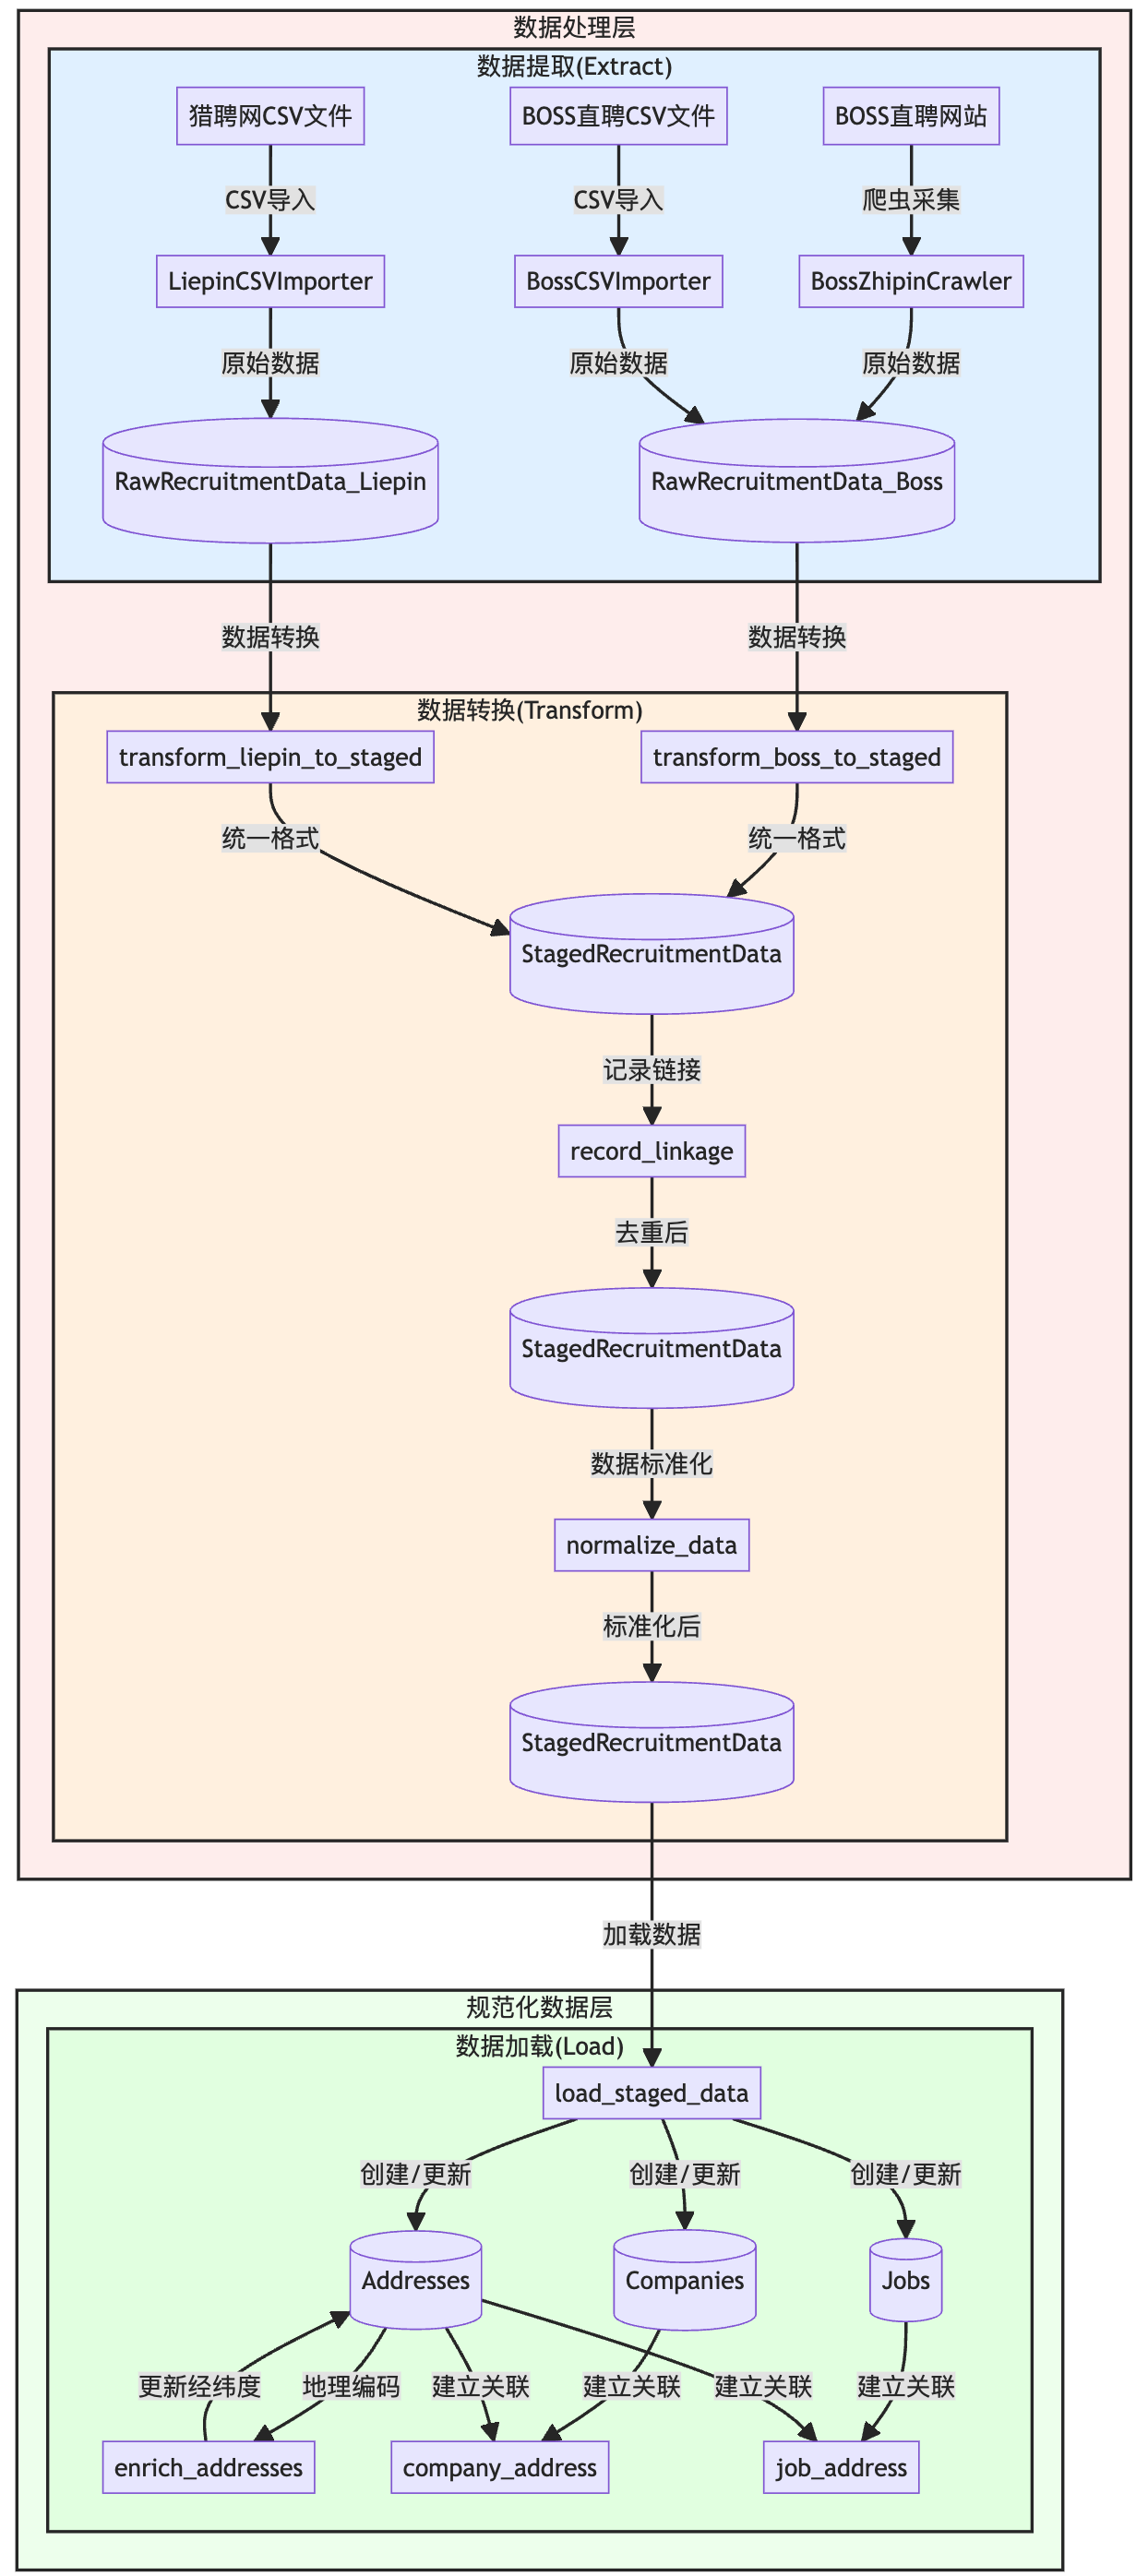
\includegraphics[width=0.6\textwidth]{figures/ETL.png}
    \caption{ETL数据集成流程}
    \label{fig:ETL}
\end{figure}

\subsubsection{数据抽取(Extract)}
数据抽取阶段主要通过两种方式获取数据,如图\ref{fig:ETL_extract}所示。包含下面两个步骤:

\begin{figure}[htbp]
    \centering
    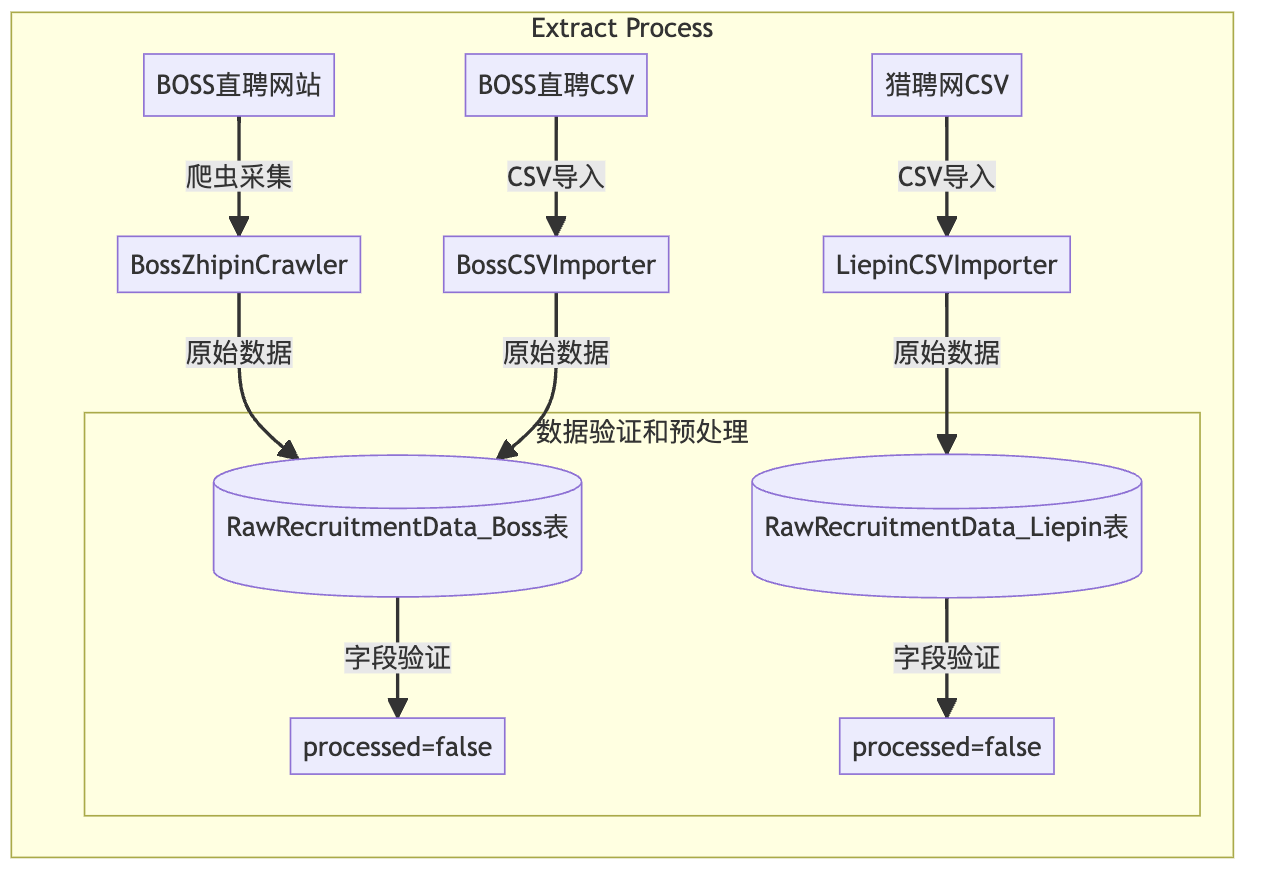
\includegraphics[width=0.5\textwidth]{figures/extract.png}
    \caption{数据抽取流程}
    \label{fig:ETL_extract}
\end{figure}


\begin{itemize}
    \item \textbf{Boss直聘数据抽取}:
    \begin{itemize}
        \item 使用Selenium实现网页爬虫,支持自动翻页和错误重试
        \item 提取职位信息、公司信息、地址等数据
        \item 数据直接存入raw\_recruitment\_boss表
    \end{itemize}
    
    \item \textbf{猎聘网数据导入}:
    \begin{itemize}
        \item 通过CSV文件导入,支持批量处理和数据验证
        \item 数据存入raw\_recruitment\_liepin表
    \end{itemize}
\end{itemize}

\subsubsection{数据转换(Transform)}
数据转换阶段是整个ETL过程中最复杂的部分,主要包括以下几个关键步骤,如图\ref{fig:ETL_transform}所示。

\begin{figure}[htbp]
    \centering
    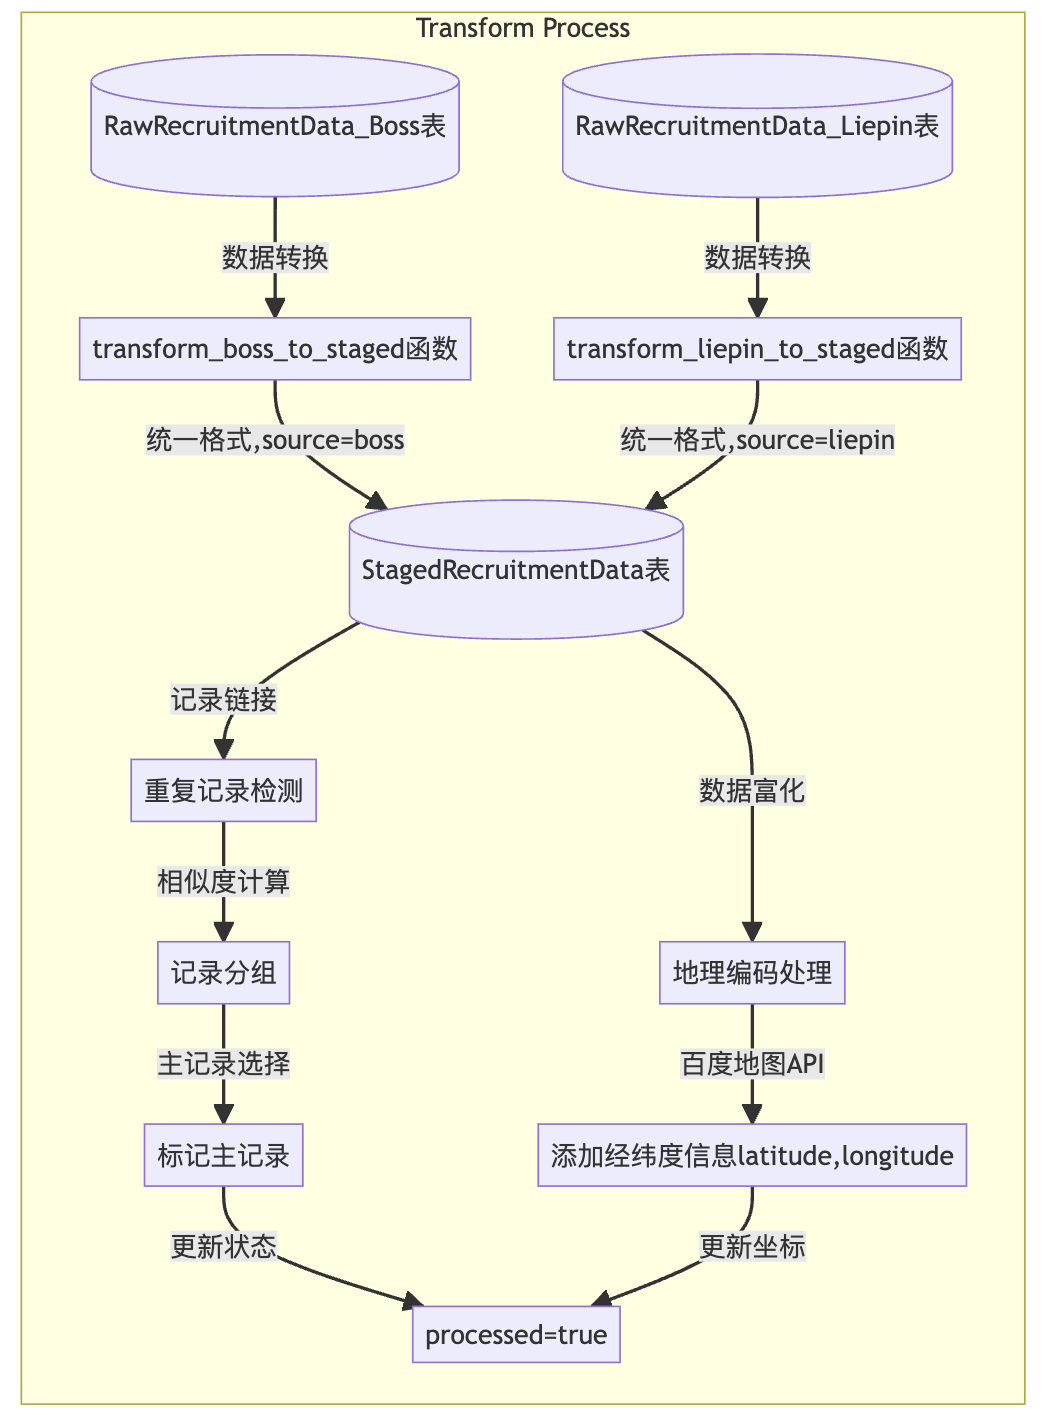
\includegraphics[width=0.5\textwidth]{figures/transform.png}
    \caption{数据转换流程}
    \label{fig:ETL_transform}
\end{figure}

数据转换过程主要包括三个部分:Boss直聘数据转换、猎聘网数据转换以及额外字段转换。如图\ref{fig:boss_transform}、图\ref{fig:liepin_transform}和图\ref{fig:extra_transform}所示。

\begin{figure}[htbp]
    \centering
    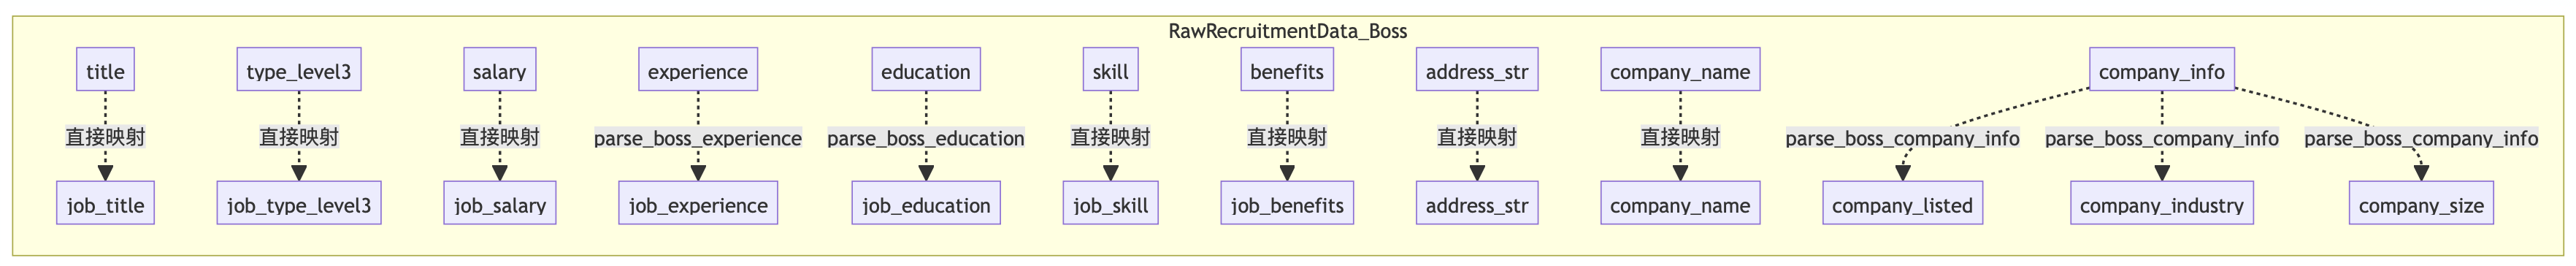
\includegraphics[width=1.0\textwidth]{figures/T过程boss.png}
    \caption{Boss直聘数据转换流程}
    \label{fig:boss_transform}
\end{figure}

从图\ref{fig:boss_transform}可以看出,Boss直聘数据的转换过程主要包括直接映射和解析转换两种方式。其中title、type\_level3、salary等字段可以直接映射到目标表,而experience、education和company\_info等字段则需要通过特定的解析函数进行转换。

\begin{figure}[htbp]
    \centering
    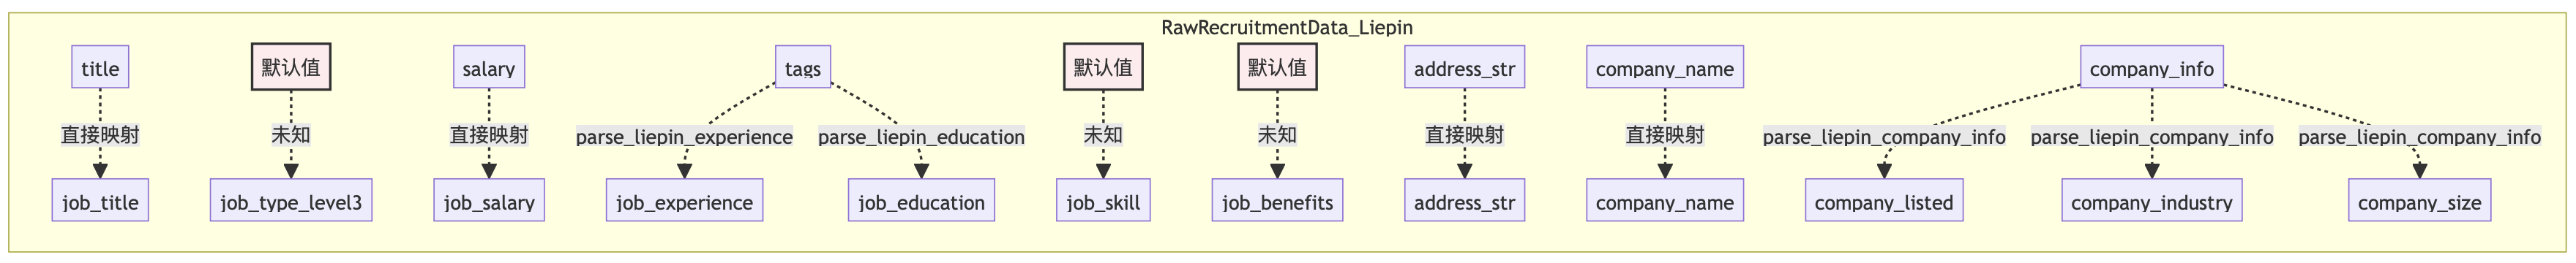
\includegraphics[width=1.0\textwidth]{figures/T过程liepin.png}
    \caption{猎聘网数据转换流程}
    \label{fig:liepin_transform}
\end{figure}

图\ref{fig:liepin_transform}展示了猎聘网数据的转换流程。由于猎聘网的数据结构与Boss直聘不同,需要针对其特有的tags字段进行解析,从中提取职位类型、工作经验、教育要求等信息。

\begin{figure}[htbp]
    \centering
    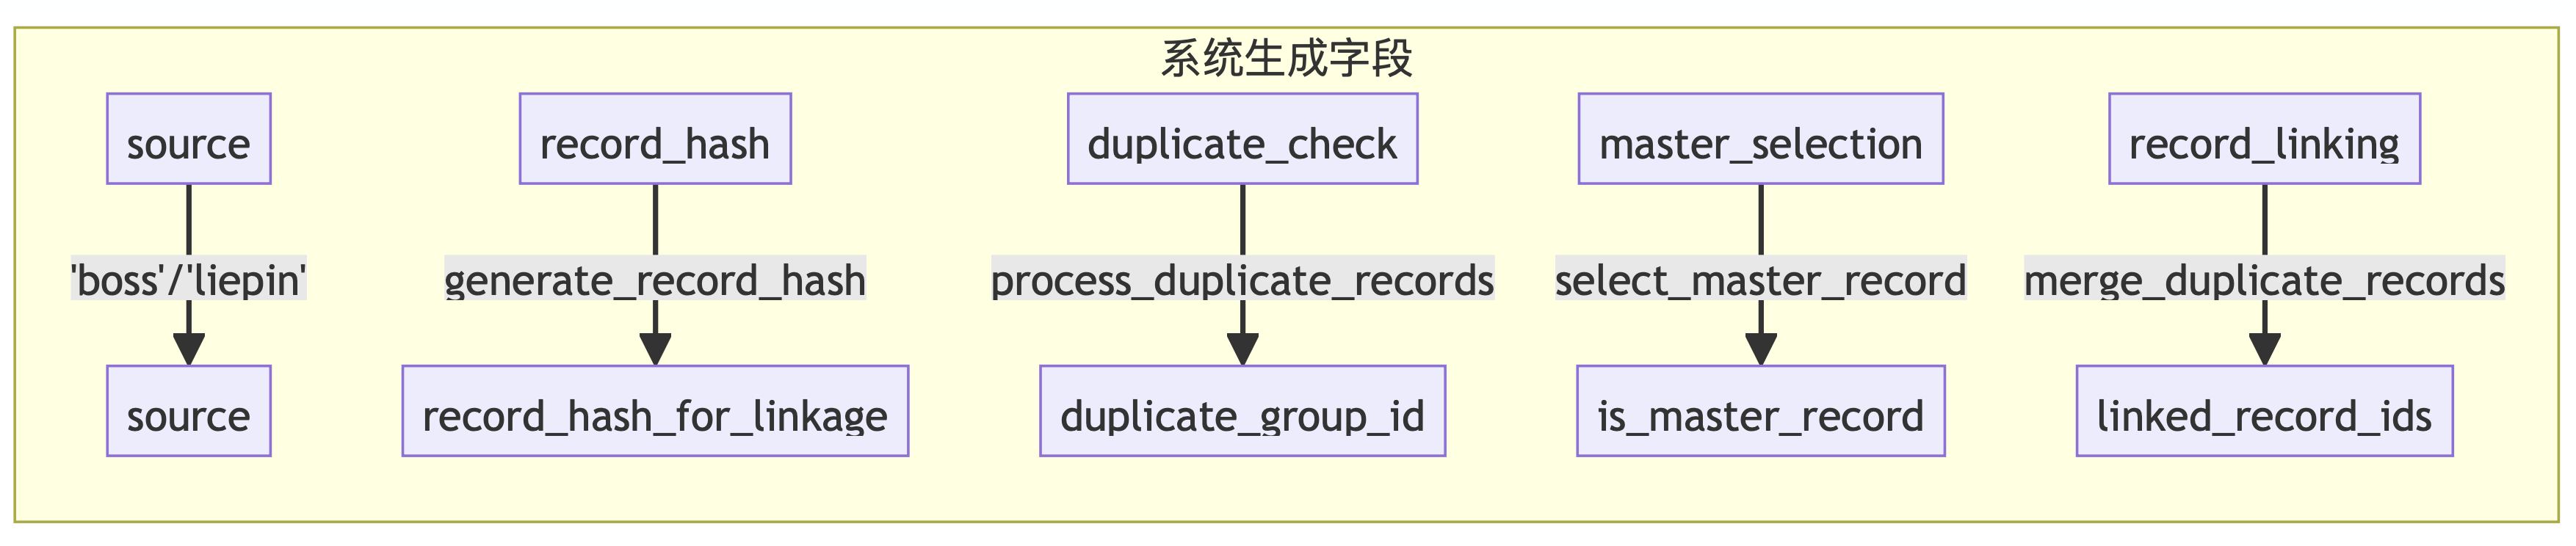
\includegraphics[width=1\textwidth]{figures/T过程extra.png}
    \caption{额外字段转换流程}
    \label{fig:extra_transform}
\end{figure}

图\ref{fig:extra_transform}显示了一些需要额外处理的字段转换过程,包括record\_hash\_for\_linkage的生成、duplicate\_group\_id的分配以及is\_master\_record的判定等。这些字段主要用于后续的记录链接和去重处理。

这个过程可以总结如下:

\begin{itemize}
    \item \textbf{数据清洗和标准化}:
    \begin{itemize}
        \item 实现了文本预处理和标准化
        \item 去除空白字符、转换英文字符为小写
        \item 移除标点符号,保留中文和英文字符
    \end{itemize}
    
    \item \textbf{记录链接和去重}:
    \begin{itemize}
        \item 采用多阶段策略进行记录链接
        \item 使用特征提取和哈希生成进行快速初筛
        \item 通过Jaccard相似度算法计算文本相似度
        \item 动态权重分配,重点关注公司名称和职位名称
    \end{itemize}
    
    \item \textbf{数据融合策略}:
    \begin{itemize}
        \item 智能选择主记录(基于记录完整度)
        \item 维护重复记录之间的关联关系
        \item 支持增量更新和批量处理
    \end{itemize}
\end{itemize}

\subsubsection{数据加载(Load)}

数据加载阶段是ETL过程的最后一个环节,负责将暂存表中的数据规范化加载到最终的数据库中。在这个阶段,系统首先会对数据进行全面的验证和预处理,包括检查必要字段的完整性、验证数据格式的正确性,以及进行必要的数据类型转换。这一步骤确保了进入最终数据库的数据都是高质量且格式统一的。

在数据验证完成后,系统会进行地理编码处理。这个过程通过调用百度地图API,将地址字符串转换为具体的经纬度坐标。系统采用了批量处理的方式提高效率,同时实现了错误重试机制以提高地理编码的成功率。对于无法成功编码的地址,系统会记录详细的错误信息,便于后续人工处理或重试。

最后是数据的规范化加载过程。这个阶段系统会根据数据库的规范化设计,将数据分别加载到不同的实体表中。首先是创建或更新公司信息,系统会检查公司是否已存在,如果存在则更新相关信息,如果不存在则创建新的公司记录。然后是处理地址信息,由于一个公司可能有多个地址,系统支持多地址的处理和存储。接着是创建职位记录,将职位相关的所有信息存入职位表中。最后,系统会建立各个实体之间的关联关系,包括公司与地址之间的关系、职位与地址之间的关系等。整个加载过程采用事务管理机制,确保数据的一致性和完整性。

为了提高数据加载的效率,系统采用了批量处理的策略,同时实现了完善的错误处理机制。当加载过程中出现异常时,系统会自动回滚事务,确保数据库的一致性不被破坏。同时,系统会详细记录每一步的处理结果,包括成功加载的记录数、失败的记录数以及具体的错误原因,这些信息对于后续的数据质量分析和系统优化都有重要的参考价值。

整个过程如图\ref{fig:ETL_load}所示。

\begin{figure}[htbp]
    \centering
    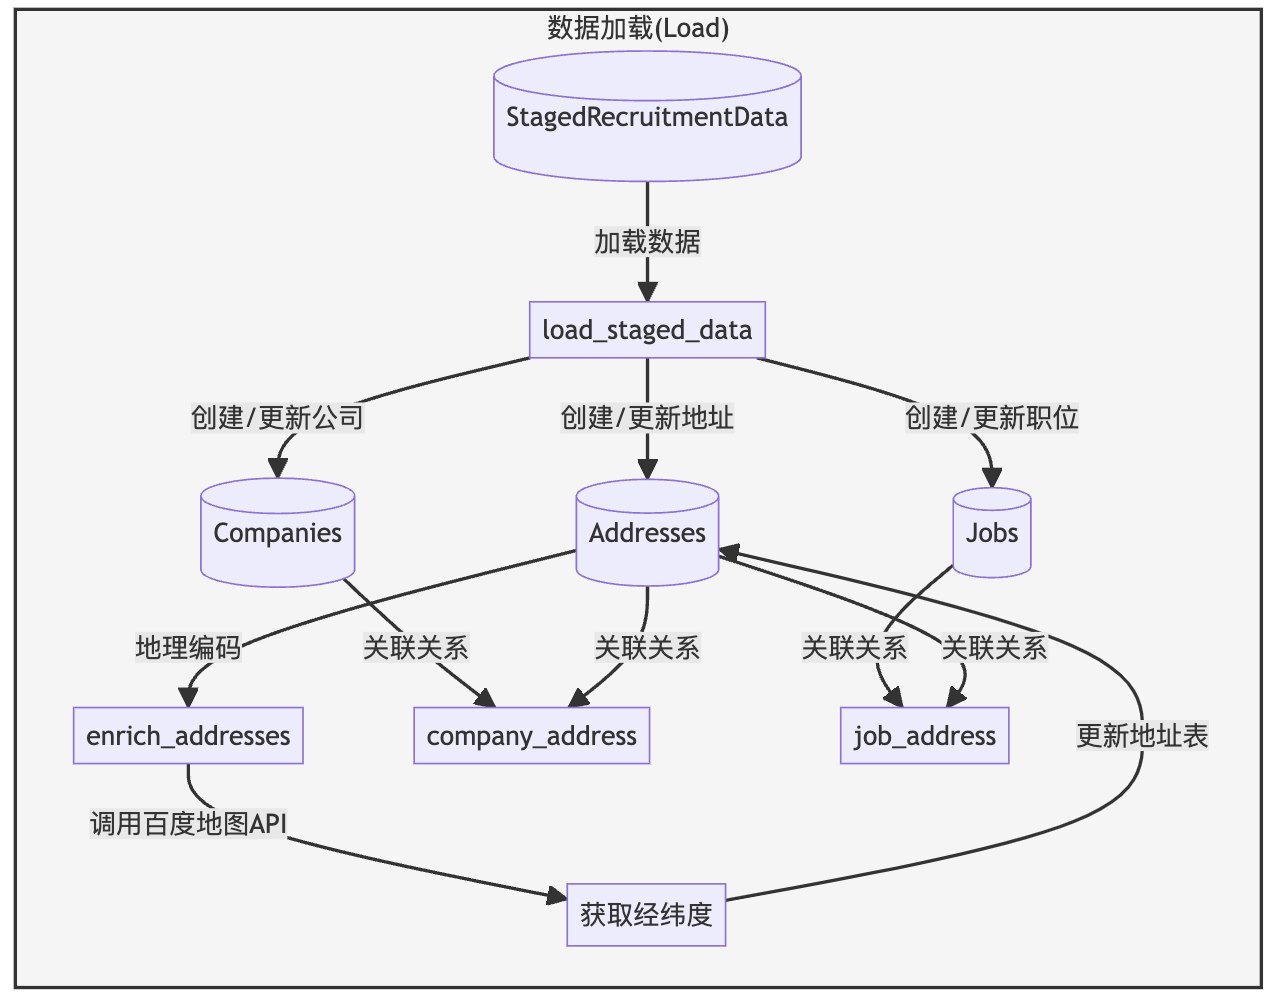
\includegraphics[width=0.5\textwidth]{figures/load.png}
    \caption{ETL数据加载流程}
    \label{fig:ETL_load}
\end{figure}

\subsubsection{CRUD层}
CRUD层作为系统的数据访问中间层,提供了统一的数据操作接口。该层的设计遵循了领域驱动设计(DDD)的原则,将业务逻辑与数据访问清晰分离:

\begin{itemize}
    \item \textbf{数据读取模块}:
    \begin{itemize}
        \item 职位数据读取:实现了高效的职位信息检索,支持多条件组合查询
        \item 公司数据读取:提供完整的公司信息访问接口,支持模糊匹配和精确查询
        \item 薪资数据读取:实现了复杂的薪资统计算法,支持多维度的薪资分析
        \item 地理数据读取:提供基于地理位置的数据检索,支持范围查询和距离计算
    \end{itemize}
    
    \item \textbf{数据解析模块}:
    \begin{itemize}
        \item 薪资解析器:采用智能算法解析多种格式的薪资描述,实现标准化处理
        \item 地址解析器:结合百度地图API,实现精确的地址解析和地理编码
        \item 数据转换解析器:提供灵活的数据转换框架,支持自定义转换规则
    \end{itemize}
    
    \item \textbf{物化视图管理}:
    \begin{itemize}
        \item 实现了智能的视图更新策略,根据数据变化频率动态调整更新周期
        \item 提供了完整的视图管理接口,支持视图的创建、更新和删除
        \item 实现了视图依赖管理,确保相关视图的同步更新
    \end{itemize}
\end{itemize}

\subsection{前端实现}

本系统的前端采用现代化的Web开发技术栈,基于采用文件路由系统的Next.js 15框架构建.


如前端项目的组件关系图\ref{fig:front_end_structure}所示,系统采用了基于Next.js的分层设计,从配置层(config.ts、globals.css、fonts.ts)到导航布局(layout.tsx)再到具体的功能页面(MapPage、FilterPage、OverviewPage)。每个功能页面都对应特定的数据可视化组件(MapPlot、FilterPlot、OverviewPlot),这些组件分别使用了不同的可视化库(Plotly.js Map、NextUI组件、Plotly.js Charts和Dashboard)来实现地图展示、数据筛选和统计概览等功能。整个前端架构通过统一的API调用(salary-distribution、filter-data、overview-stats)与后端进行数据交互,实现了清晰的数据流动和模块化的功能划分。

\begin{figure}[htbp]
    \centering
    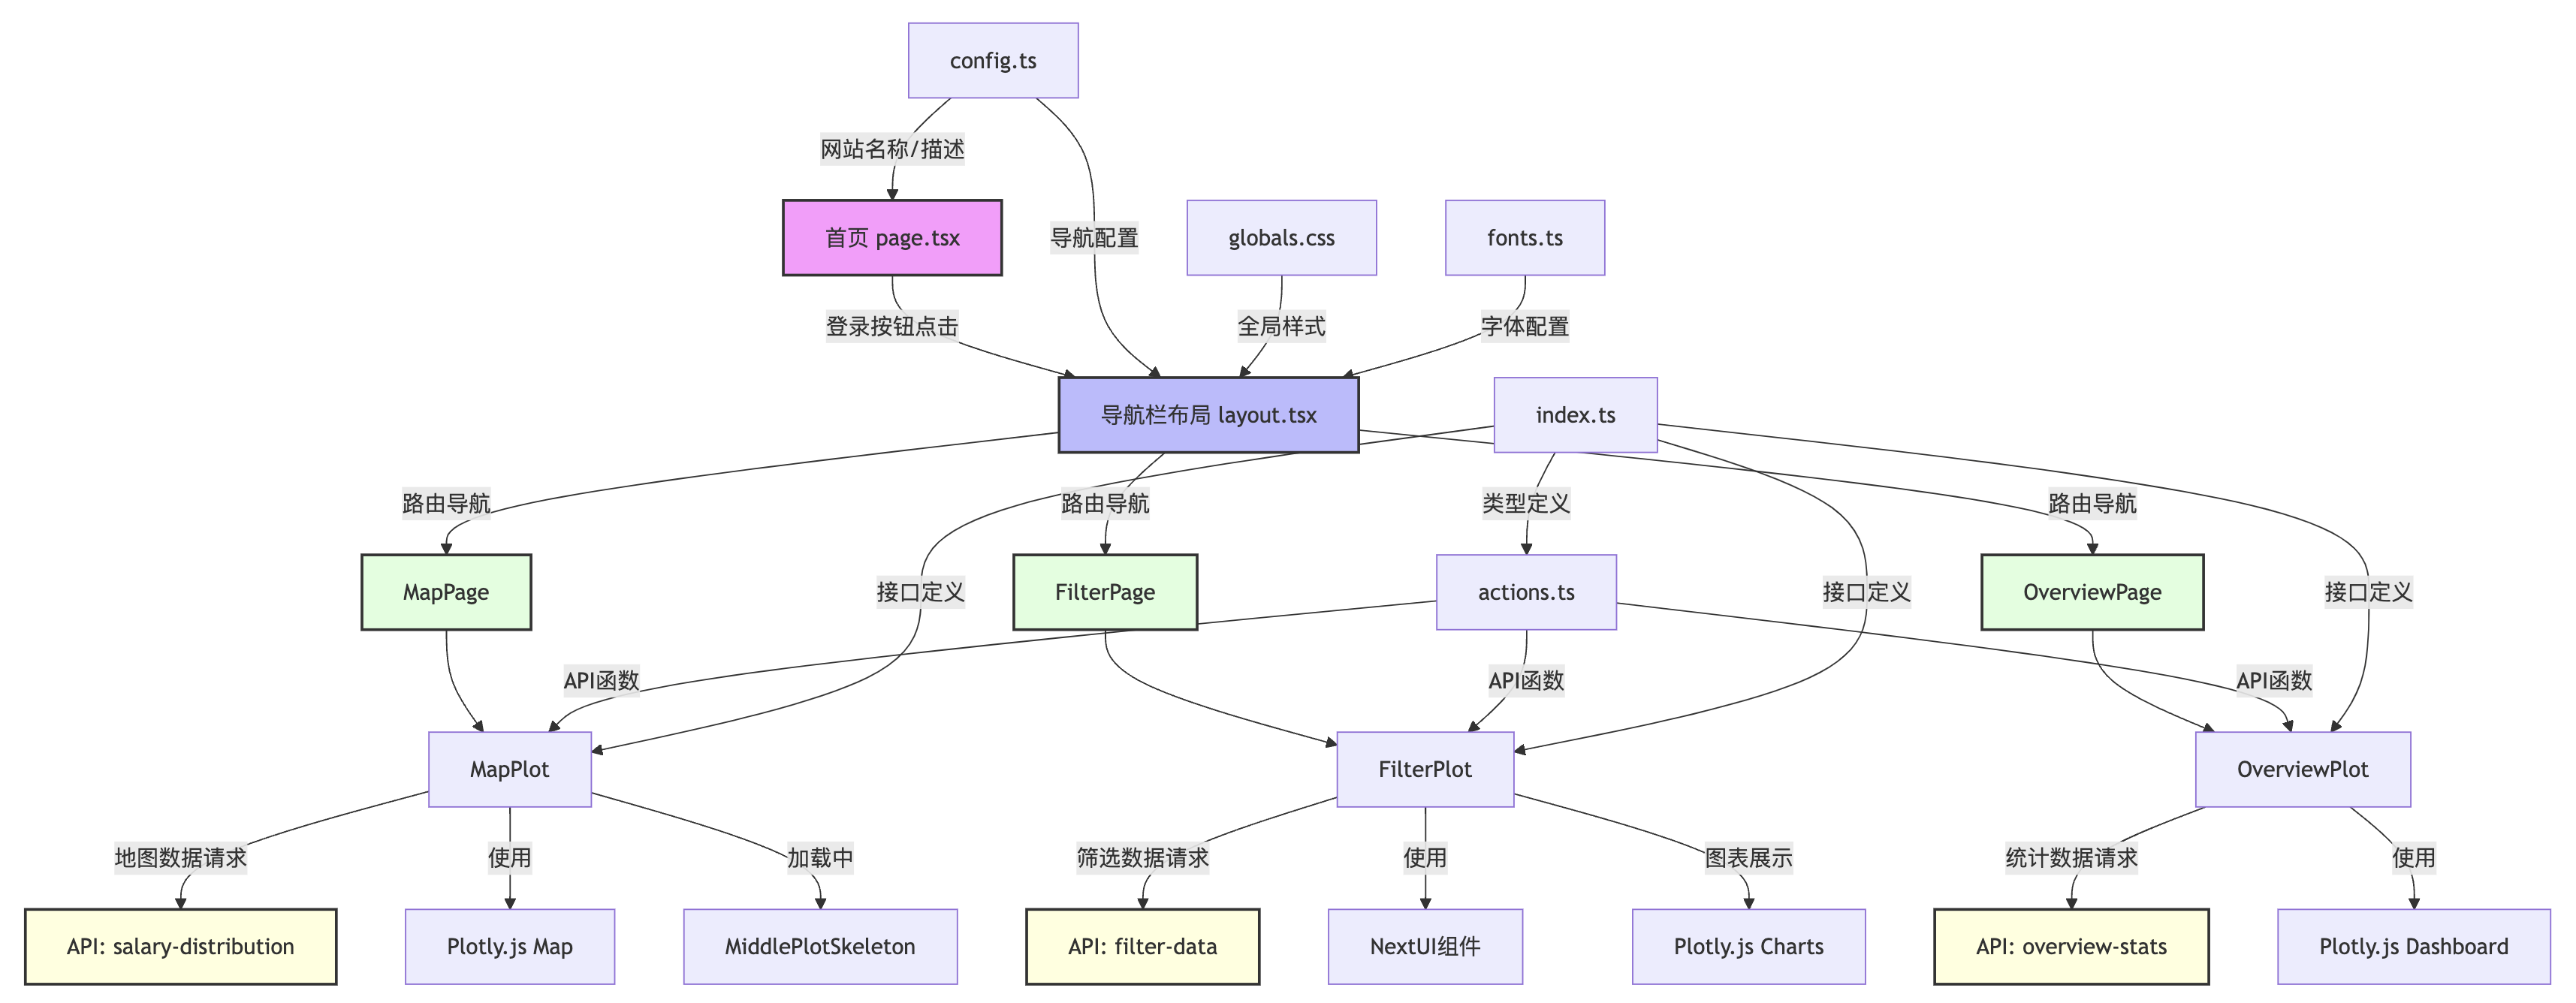
\includegraphics[width=1.0\textwidth]{figures/前端项目结构图.png}
    \caption{前端项目结构图}
    \label{fig:front_end_structure}
\end{figure}

如前端数据流图\ref{fig:front_end_data_flow}所示,系统采用了基于React Hooks的状态管理模式,从用户交互(用户点击、用户输入、用户选择)开始,通过useState和useEffect等钩子函数管理状态和副作用。数据流经过actions.ts进行统一的动作处理,然后通过fetch请求调用后端API。获取的数据经过数据解析和TypeScript类型转换后,最终通过Plotly.js或NextUI组件进行可视化展示,同时系统还实现了错误处理和加载状态显示,形成了一个完整的前端数据处理闭环。这种设计保证了数据流的单向性和可预测性,提高了应用的可维护性和性能。


\begin{figure}[htbp]
    \centering
    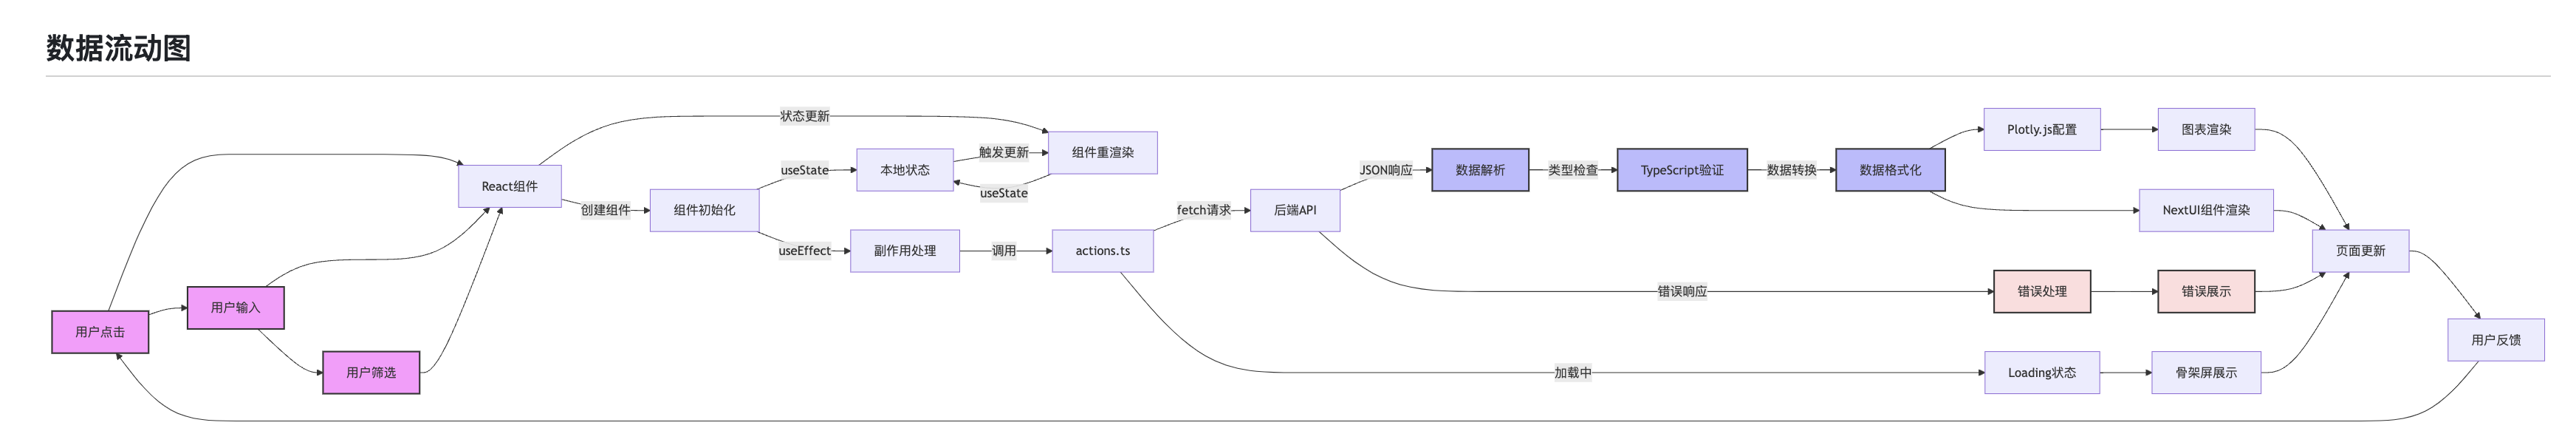
\includegraphics[width=1.0\textwidth]{figures/前端数据流图.png}
    \caption{前端数据流图}
    \label{fig:front_end_data_flow}
\end{figure}


\section{测试数据}


\subsection{测试数据概述}
系统中的数据存储结构清晰,各表之间关系合理,主要包含以下数据表:

\begin{itemize}
    \item \textbf{原始数据表}:
    \begin{itemize}
        \item raw\_recruitment\_boss:存储BOSS直聘平台的原始招聘数据,容量56 MB,包含18,290条记录
        \item raw\_recruitment\_liepin:存储猎聘网的原始招聘数据,容量304 kB,包含220条记录
    \end{itemize}
    
    \item \textbf{核心业务表}:
    \begin{itemize}
        \item jobs:职位信息表,容量9,384 kB,包含18,166条记录
        \item recruitment\_mv:招聘信息物化视图,容量8,432 kB,包含18,166条记录
        \item companies:公司信息表,容量2,504 kB,包含8,691条记录
    \end{itemize}
    
    \item \textbf{地址相关表}:
    \begin{itemize}
        \item job\_address:职位地址关联表,容量1,240 kB,包含18,166条记录
        \item company\_address:公司地址关联表,容量784 kB,包含10,205条记录
        \item addresses:标准化地址表,容量256 kB,包含329条记录
    \end{itemize}

\end{itemize}


从数据规模来看,系统主要以BOSS直聘数据为主,辅以少量猎聘网数据。数据表之间的记录数量关系合理,反映了正确的业务关联。例如,一个职位对应一条地址记录(job\_address与jobs记录数相同),而一个公司可能有多个地址(company\_address记录数大于companies)。系统整体数据质量良好,表结构设计合理,为应用功能提供了可靠的数据基础。

\subsection{界面展示}

\subsubsection{MapPage 地图页面}
如图\ref{fig:map_page}所示,MapPage是一个专注于地理数据可视化的界面,其核心功能是展示各地区的薪资分布情况。同时提供区域薪资水平和热力图两种不同的地图视图模式,让用户能够直观且全面地了解不同地区的薪资水平分布状况。


\begin{figure}[htbp]
    \centering
    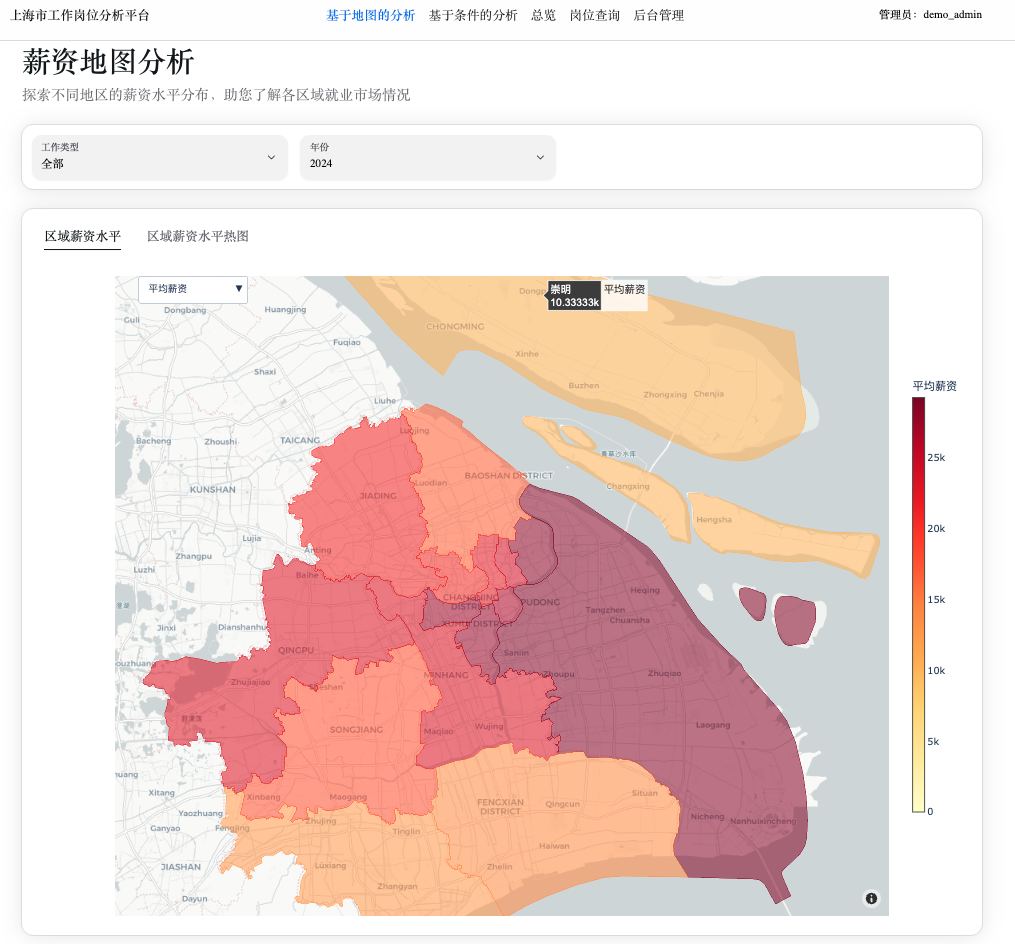
\includegraphics[width=1.0\textwidth]{figures/map_page.png}
    \caption{地图页面}
    \label{fig:map_page}
\end{figure}

\begin{figure}[htbp]
    \centering
    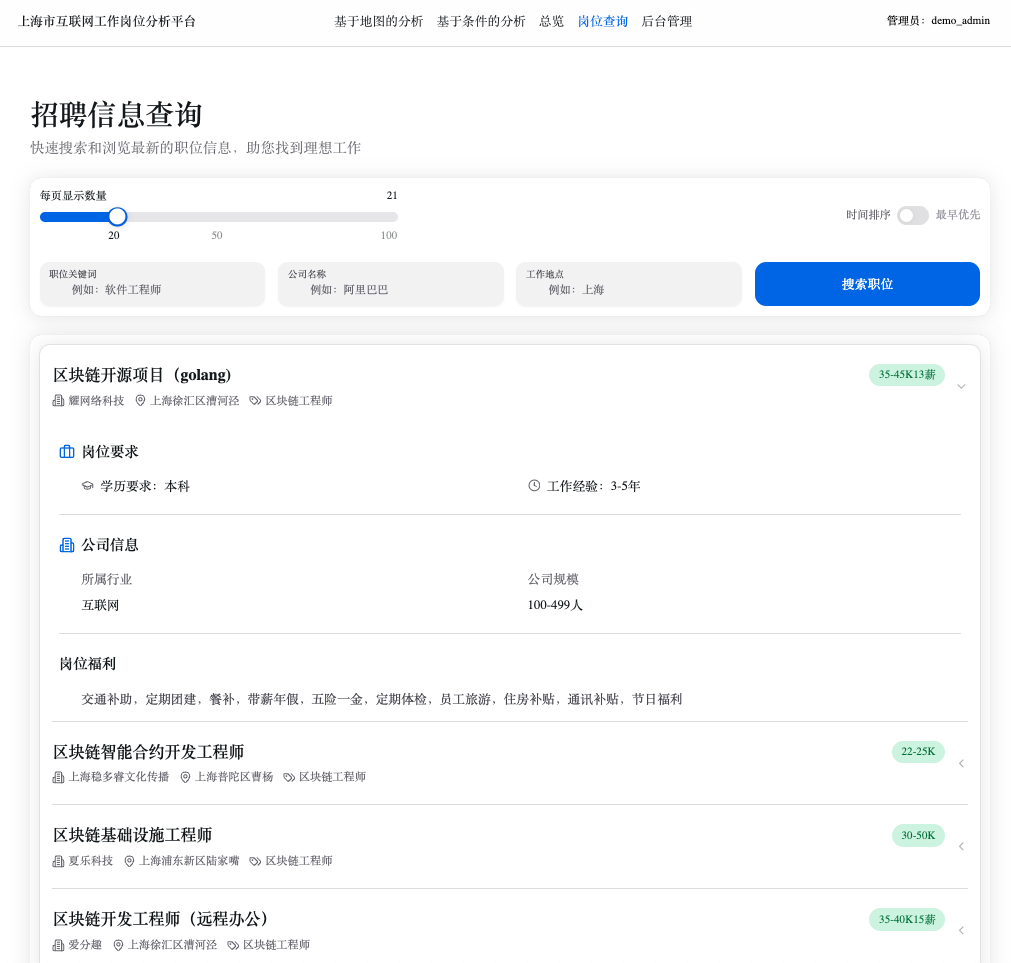
\includegraphics[width=1.0\textwidth]{figures/recruitment_page.png}
    \caption{招聘信息页面}
    \label{fig:recruitment_page}
\end{figure}

\begin{figure}[htbp]
    \centering
    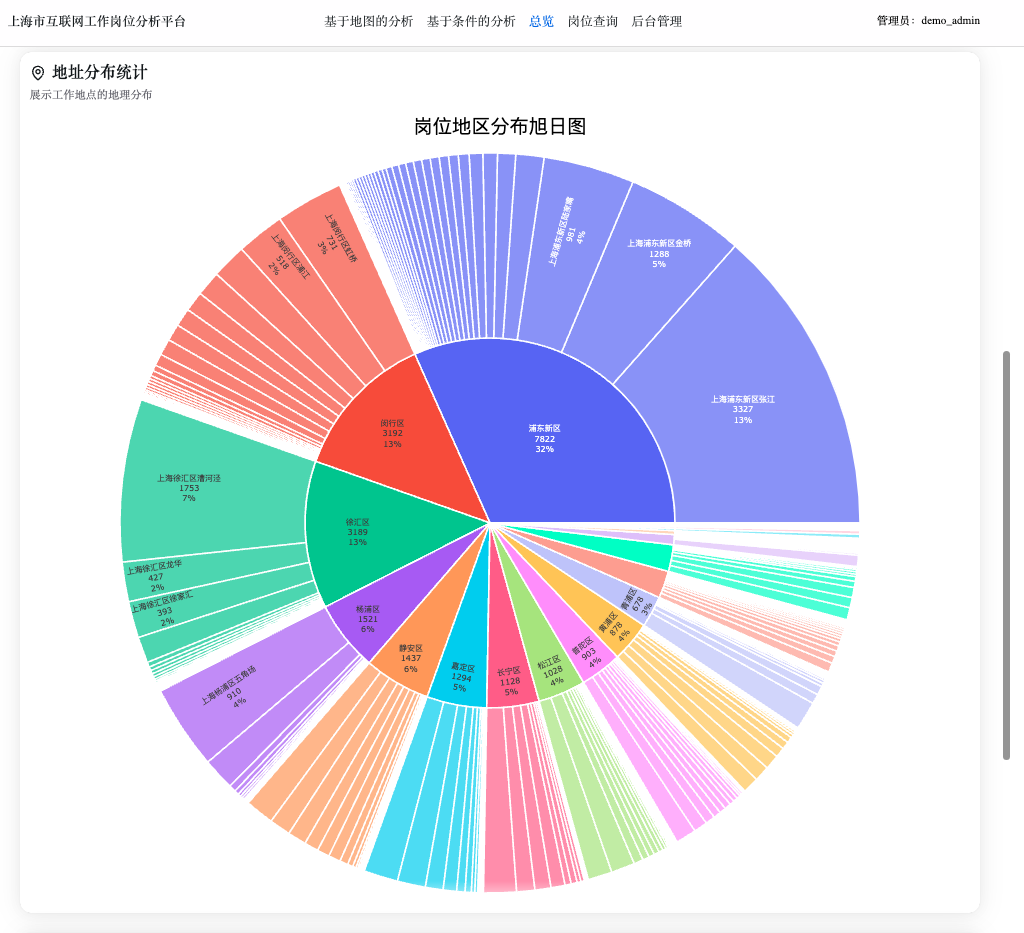
\includegraphics[width=1.0\textwidth]{figures/overview_page.png}
    \caption{概览页面}
    \label{fig:overview_page}
\end{figure}

\begin{figure}[htbp]
    \centering
    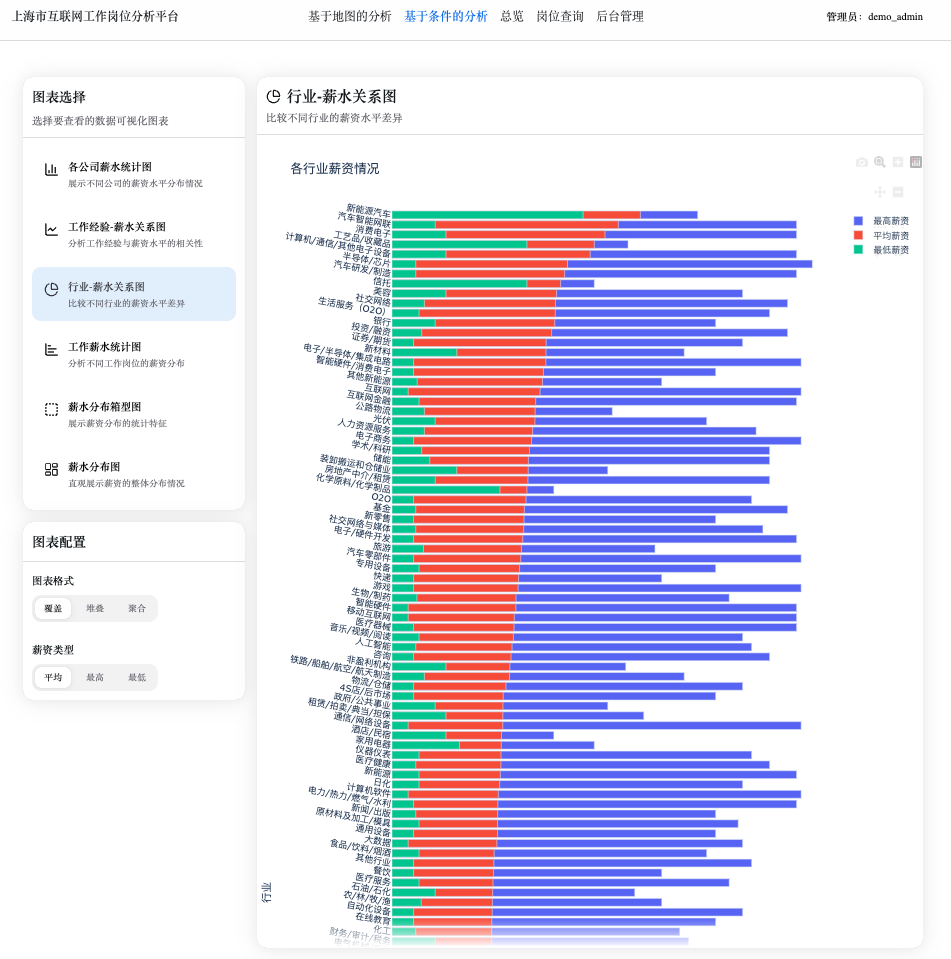
\includegraphics[width=1.0\textwidth]{figures/filter_page.png}
    \caption{筛选分析页面}
    \label{fig:filter_page}
\end{figure}

\begin{figure}[htbp]
    \centering
    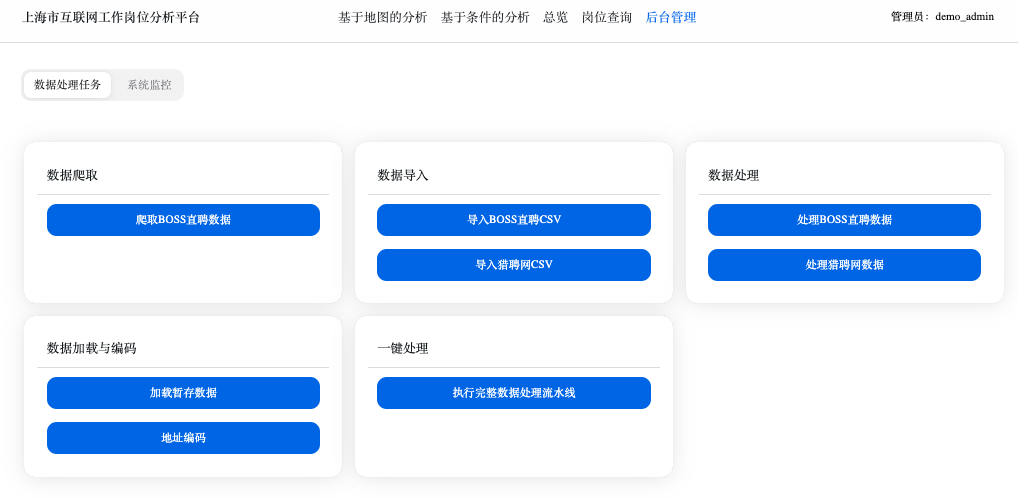
\includegraphics[width=1.0\textwidth]{figures/task_page1.png}
    \caption{任务管理页面}
    \label{fig:task_page_1}
\end{figure}

\begin{figure}[htbp]
    \centering
    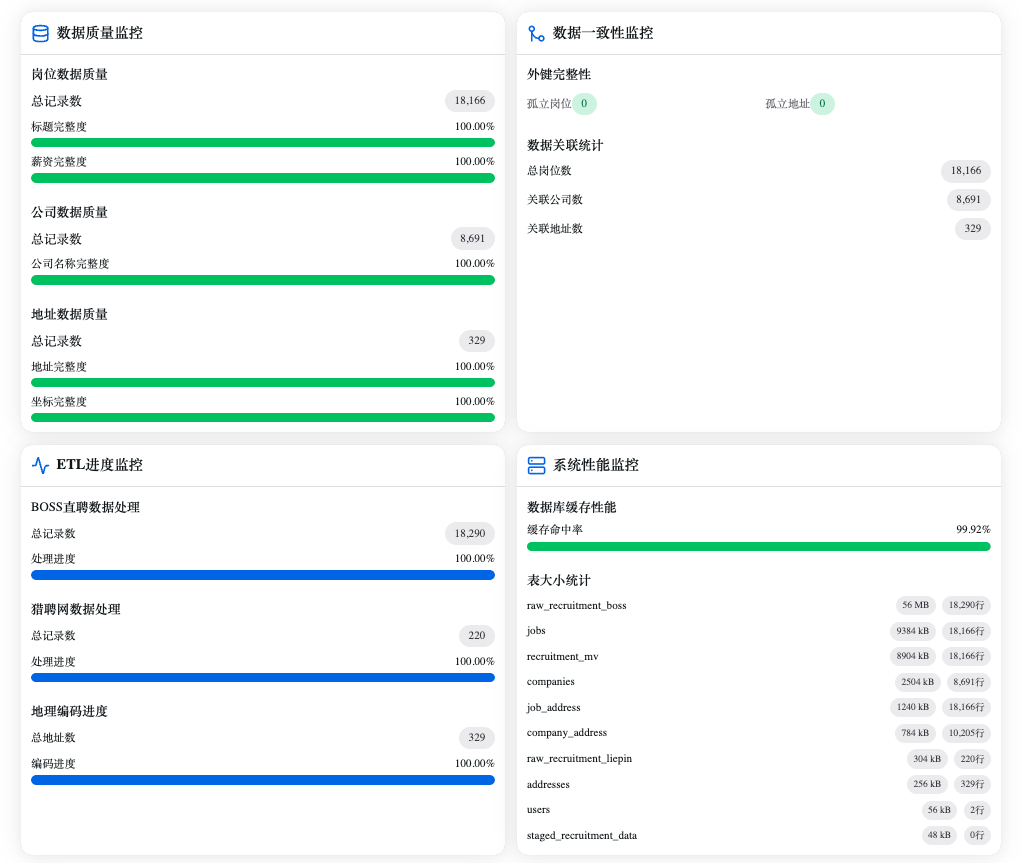
\includegraphics[width=1.0\textwidth]{figures/task_page2.png}
    \caption{系统监控页面}
    \label{fig:task_page_2}
\end{figure}


\subsubsection{RecruitmentPage 招聘信息页面}
如图\ref{fig:recruitment_page}所示,RecruitmentPage是一个功能完备的招聘信息查询平台,为用户提供精确的职位搜索体验。用户可以通过输入职位关键词、公司名称和工作地点等条件进行精确搜索,并可以灵活调整每页显示的信息数量(范围从1到100条)以及选择按时间的排序方式(最新或最早优先)。所有招聘信息都以清晰的卡片形式呈现,每张卡片都包含详尽的公司信息、具体的岗位要求以及完整的福利待遇说明。

\subsection{OverviewPage 概览页面}
如图\ref{fig:overview_page}所示,OverviewPage作为数据总览平台,通过丰富的数据可视化图表全方位展示就业市场概况。页面集中呈现了职位分布、地址分布、教育经验分布等多个维度的统计信息,并配备了直观的滑块控件,允许用户自由调整显示的职位数量(范围从1到200个),帮助用户快速准确地把握当前就业市场的整体态势。

\subsubsection{FilterPage 筛选分析页面}
如图\ref{fig:filter_page}所示,FilterPage是为用户提供深度的数据洞察能力。页面整合了多种专业的数据可视化图表,包括详细的公司薪资统计、经验与薪资的关系分析、行业薪资分布等核心指标。用户可以根据需求选择不同的图表类型,并通过调整展示模式(覆盖、堆叠或聚合)、薪资类型(平均值、最高值或最低值)以及学历条件等参数,进行全方位的数据分析。

\subsection{TaskPage 任务管理页面}
如图\ref{fig:task_page_1}所示,TaskPage的数据处理任务是一个面向管理员的专业数据处理任务管理平台,提供全面的数据管理功能。界面采用直观的卡片式布局,系统地组织各类数据任务,包括BOSS直聘平台的数据爬取、BOSS直聘和猎聘网的数据导入、数据处理以及地址编码等核心功能。特别设计了一键式操作选项,支持执行完整的数据处理流水线,大大提高了数据管理的效率和便捷性。

如图\ref{fig:task_page_2}所示,系统监控页面全面展示了数据处理和存储的运行状况:在数据质量方面,系统共处理了18,284条岗位数据、8,689条公司数据和330条地址数据,各项数据的完整度均达到100\%;在数据一致性方面,系统中没有出现孤立的岗位和地址记录,确保了数据的关联完整性;在ETL处理方面,BOSS直聘的18,290条数据和猎聘网的220条数据均已完成处理,地理编码任务也已全部完成;在系统性能方面,数据库存储使用率达到99.91\%,各数据表大小合理分布,从raw\_recruitment\_boss表的56MB到users表的56KB不等,整体运行状态良好。




\section{小组分工}
本项目小组分工明确,采用GitHub来实现协同开发。
各成员对于项目的贡献度均为50\%。具体分工如下:

\begin{enumerate}
    \item 郑辉阳:数据集成与后端;
    \item 范潇:数据采集与前端。
\end{enumerate}
\chapter{总结}
\thispagestyle{empty}
\section{心得体会}
通过本次项目,我收获颇丰。

其一,我通过数据库的设计过程进一步加深了对于上一学期中所学理论知识的理解。

其二,我对于数据库在实际开发过程中的使用有了较为全面的了解。我在本项目中,通过多种方式来和数据交互:
在使用数据来填充数据库的过程中,我使用Python语言来与数据库进行交互;在应用开发过程中,我使用DataGrip和pgAdmin4来对于
数据库进行管理;在应用开发阶段,我是用Drizzle ORM来进行数据的CRUD操作。同时,本项目所使用的数据库涉及到
多种数据类型,例如\textbf{ENUM},\textbf{TEXT},\textbf{point},被用来存储单车状态,图片和坐标等信息;本项目还利用
数据库提供的\verb|crypt|函数来实现对于用户密码的加密存储、利用\textbf{check}约束和触发器来确保数据的一致性;本项目
还利用数据库中的用户定义函数来实现添加用户功能。

其三,通过本次项目我也掌握了开发网页的基本流程的技术栈。对于前端,我学习了React和Tailwind CSS的基本使用方法;
对于后端,我了解了ORM技术、鉴权技术以及Typescript语言的基本使用。同时,我还对于App路由版本的Next.js有了初步了解,
能够利用它来快速开发出一个中小型网页应用。
\section{数据采集与集成的国内外现状认识与体会}

在数据采集方面,国内外的发展情况有较大的差别,其主要原因是我国互联网行业起步相对较慢。
一方面,在数据源头层面,我国各地政府以及官方机构
公开数据的渠道较少,且多数存在质量低、数据量少、更新频率低等问题,使得我国缺少了一高质量数据来源;
另一方面,在软件生态层面,常用的requests,beautiful soup,scrapy等库都来自国外,并且经过了长期的开发,具有完善的功能。
例如requests库有Kenneth Reitz于2011年创建、BeautifulSoup由Leonard Richardson开发,初版发布于2004年;Scrapy由Scrapinghub开发,发布时间为2008。
近年来,由于大模型的兴起而导致的对于大规模数据的需求推动了数据采集的发展,
例如LAION数据集的采集催生出了img2dataset这一高性能的网络图像爬取库。


在数据集成方面,我国以阿里巴巴、字节跳动等公司推出了多款开源的数据集成工具,例如阿里巴巴的Addax、字节跳动开源的BitSail、云雀等。

我认为我国需加强对于数据公开平台的规范化建设,应该把握住由于庞大的人口所带来的数据资源,加速发展数据采集与集成技术。

% \section*{谢辞}
\addcontentsline{toc}{section}{谢辞}

本节通常用于感谢在研究过程中给予帮助和支持的人们,例如指导老师、实验室同学、朋友和家人等。

在谢辞中,需要真诚地表达感谢之情,回顾一下在研究过程中所受到的帮助和支持,并提到他们的具体贡献和重要性。同时,也可以简要说明一下自己在研究过程中的收获和体会,表达对他们的感激之情和祝福。

最后,需要注意不要出现太多的感情用词,语言简洁明了,表达真诚和诚恳即可。

谢谢支持本项目的所有朋友们。并且希望选用该模板的朋友们都能顺利通过查重与答辩。


\end{document}
